%%%%%%%%%%%%%%%%%%%%%%%%%%%%%%%%%%%%%%%%%%%%%%%%%%%%%%%%%%%%%%%%%%%%%%%
%
%   MODIF DU TEMPLATE DE NICO
%
%%%%%%%%%%%%%%%%%%%%%%%%%%%%%%%%%%%%%%%%%%%%%%%%%%%%%%%%%%%%%%%%%%%%%%%%
% !TEX encoding = MacOSRoman
\documentclass[a4paper, 12pt]{report}

\usepackage{latexsym}
\usepackage{graphicx}
\usepackage{amsfonts}
\usepackage{amsmath}
\usepackage{amssymb}
\usepackage{xcolor}
\usepackage{tablefootnote}

%\usepackage{draftwatermark}
%\SetWatermarkText{DRAFT}
%\SetWatermarkScale{5}


%-----------------------------------------
% Pour accepter les lettres accentuees de clavier azerty
% sans les é (utile) pour tapper directement en azerty 
% et ou faire passer aspell -c --lang=fr bidon.tex
\usepackage[utf8]{inputenc}
%\usepackage[applemac]{inputenc} %c'est ca qui gère les accents d'après un forum
%------------------------------------------
\usepackage{natbib}
\bibpunct{(}{)}{;}{a}{}{,} % to follow the A&A style

% copie de aa.cls
%-----------------------------------
\newcommand*\aap{A\&A}
\let\astap=\aap
\newcommand*\aapr{A\&A~Rev.}
\newcommand*\aaps{A\&AS}
\newcommand*\actaa{Acta Astron.}
\newcommand*\aj{AJ}
\newcommand*\ao{Appl.~Opt.}
\let\applopt\ao
\newcommand*\apj{ApJ}
\newcommand*\apjl{ApJ}
\let\apjlett\apjl
\newcommand*\apjs{ApJS}
\let\apjsupp\apjs
\newcommand*\aplett{Astrophys.~Lett.}
\newcommand*\apspr{Astrophys.~Space~Phys.~Res.}
\newcommand*\apss{Ap\&SS}
\newcommand*\araa{ARA\&A}
\newcommand*\azh{AZh}
\newcommand*\baas{BAAS}
\newcommand*\bac{Bull. astr. Inst. Czechosl.}
\newcommand*\bain{Bull.~Astron.~Inst.~Netherlands}
\newcommand*\caa{Chinese Astron. Astrophys.}
\newcommand*\cjaa{Chinese J. Astron. Astrophys.}
\newcommand*\fcp{Fund.~Cosmic~Phys.}
\newcommand*\gca{Geochim.~Cosmochim.~Acta}
\newcommand*\grl{Geophys.~Res.~Lett.}
\newcommand*\iaucirc{IAU~Circ.}
\newcommand*\icarus{Icarus}
\newcommand*\jcap{J. Cosmology Astropart. Phys.}
\newcommand*\jcp{J.~Chem.~Phys.}
\newcommand*\jgr{J.~Geophys.~Res.}
\newcommand*\jqsrt{J.~Quant.~Spectr.~Rad.~Transf.}
\newcommand*\jrasc{JRASC}
\newcommand*\memras{MmRAS}
\newcommand*\memsai{Mem.~Soc.~Astron.~Italiana}
\newcommand*\mnras{MNRAS}
\newcommand*\na{New A}
\newcommand*\nar{New A Rev.}
\newcommand*\nat{Nature}
\newcommand*\nphysa{Nucl.~Phys.~A}
\newcommand*\pasa{PASA}
\newcommand*\pasj{PASJ}
\newcommand*\pasp{PASP}
\newcommand*\physrep{Phys.~Rep.}
\newcommand*\physscr{Phys.~Scr}
\newcommand*\planss{Planet.~Space~Sci.}
\newcommand*\pra{Phys.~Rev.~A}
\newcommand*\prb{Phys.~Rev.~B}
\newcommand*\prc{Phys.~Rev.~C}
\newcommand*\prd{Phys.~Rev.~D}
\newcommand*\pre{Phys.~Rev.~E}
\newcommand*\prl{Phys.~Rev.~Lett.}
\newcommand*\procspie{Proc.~SPIE}
\newcommand*\qjras{QJRAS}
\newcommand*\rmxaa{Rev. Mexicana Astron. Astrofis.}
\newcommand*\skytel{S\&T}
\newcommand*\solphys{Sol.~Phys.}
\newcommand*\sovast{Soviet~Ast.}
\newcommand*\ssr{Space~Sci.~Rev.}
\newcommand*\zap{ZAp}
%-------------------------------------------------


\usepackage[french]{babel} % pour avoir chapitre plutôt que "chapter", peut-être la ponctuation aussi...

%page de couverture du manuscrit
\usepackage{meta-donnees}

% COLOR
\definecolor{mypink}{rgb}{1.0,0.0,0.5}
\definecolor{myblue}{rgb}{0.0,0.0,1.0}
\definecolor{mygrey}{rgb}{0.3,0.3,0.3}

%\definecolor{darkblue}{rgb}{0.12,0.47,0.87}
%\definecolor{darkblue}{rgb}{0.07,0.34,0.6}
\definecolor{bleu}{RGB}{30,144,255}
\definecolor{bleumarine}{RGB}{0,89,179}
\definecolor{bleu2}{RGB}{26,102,255}
\definecolor{bleumarine2}{RGB}{0,60,179}
\definecolor{orange}{RGB}{255,200,0}%{255,77,0}
\definecolor{vert}{RGB}{60,180,0}
\usepackage{twoopt}


%  AJOUT LP
\usepackage[T1]{fontenc}
\usepackage[explicit]{titlesec}
\usepackage[protrusion=true,expansion=true]{microtype} % Better typography
\usepackage{tablefootnote} % to display footnotes in tables
\usepackage{threeparttable}
\usepackage[toc,page]{appendix}
\usepackage{multirow}
\usepackage{mathpazo} % Use the Palatino font
\linespread{1.05} % Change line spacing here, Palatino benefits from a slight increase by default
%\usepackage[bjornstrup]{fncychap}
\usepackage{minitoc}
\usepackage{anyfontsize}
\usepackage{lipsum}
\usepackage{overpic}

%hyperref must come last of all the used package because it redefines latex commands such as \section...
\usepackage[colorlinks,
	urlcolor=mygrey,
	linkcolor=bleu2,
        citecolor=bleumarine2,
	breaklinks=true]{hyperref}

% FORMAT DES SECTIONS
%\newlength\chapnumb
%\setlength\chapnumb{4cm}

%\titleformat{command}[shape]{format}{label}{sep}{before-code}[after-code]]

\titleclass{\part}{top} % make part like a chapter
\titleformat{\part}
[display]
{\normalfont\sffamily\Huge\bfseries}
{\parbox[b]{\dimexpr\textwidth}{\vspace{-1cm}
    \raggedleft
    \color{bleu}\bfseries\fontsize{36}{36}\selectfont\partname \thepart}\vspace{2cm}}
{0pt}
{\LARGE #1}

%\titlespacing*{\part}{0pt}{0pt}{20pt}

\titleformat{\chapter}[display] {
  \normalfont\sffamily}{
  \parbox[b]{\dimexpr\textwidth}{\vspace{-1cm}
    \raggedleft
    \color{bleu}\bfseries\fontsize{72}{72}\selectfont\thechapter}\vspace{0.5cm}
}{0pt}{{\LARGE#1}%\\
  %\rule{\dimexpr\textwidth}{0.4pt}
}

\titleformat{name=\chapter,numberless}[display] {
  \normalfont\sffamily}{}{0pt}{
  \parbox[b]{\dimexpr\textwidth}{
    \raggedleft
    \LARGE #1}%\\
  %\rule{\dimexpr\textwidth}{0.4pt}
}



% SPECIAL COMMANDS  
\makeatletter
%\newcommandtwoopt{\citeads}[3][][]{\href{http://adsabs.harvard.edu/abs/#3}{\def\hyper@linkstart##1##2{}\let\hyper@linkend\@empty\citealp[#1][#2]{#3}}}
%\newcommandtwoopt{\citepads}[3][][]{\href{http://adsabs.harvard.edu/abs/#3}{\def\hyper@linkstart##1##2{}\let\hyper@linkend\@empty\citep[#1][#2]{#3}}}
%\newcommandtwoopt{\citetads}[3][][]{\href{http://adsabs.harvard.edu/abs/#3}{\def\hyper@linkstart##1##2{}\let\hyper@linkend\@empty\citet[#1][#2]{#3}}}

\newcommandtwoopt{\tempciteads}[3][][]{\href{http://adsabs.harvard.edu/abs/#3}{\def\hyper@linkstart##1##2{}\let\hyper@linkend\@empty\citealp[#1][#2]{#3}}}
\newcommandtwoopt{\tempcitepads}[3][][]{\href{http://adsabs.harvard.edu/abs/#3}{\def\hyper@linkstart##1##2{}\let\hyper@linkend\@empty\citep[#1][#2]{#3}}}
\newcommandtwoopt{\tempcitetads}[3][][]{\href{http://adsabs.harvard.edu/abs/#3}{\def\hyper@linkstart##1##2{}\let\hyper@linkend\@empty\citet[#1][#2]{#3}}}


\newcommandtwoopt{\citealpads}[3][][]{\href{http://adsabs.harvard.edu/abs/#3}{\def\hyper@linkstart##1##2{}\let\hyper@linkend\@empty\citealp[#1][#2]{#3}}}
\newcommandtwoopt{\citealtads}[3][][]{\href{http://adsabs.harvard.edu/abs/#3}{\def\hyper@linkstart##1##2{}\let\hyper@linkend\@empty\citealt[#1][#2]{#3}}}
\newcommandtwoopt{\citeyearads}[3][][]{\href{http://adsabs.harvard.edu/abs/#3}{\def\hyper@linkstart##1##2{}\let\hyper@linkend\@empty\citeyear[#1][#2]{#3}}}
\newcommandtwoopt{\citeadsstar}[3][][]{\href{http://adsabs.harvard.edu/abs/#3}{\def\hyper@linkstart##1##2{}\let\hyper@linkend\@empty\citealp*[#1][#2]{#3}}}
\newcommandtwoopt{\citepadsstar}[3][][]{\href{http://adsabs.harvard.edu/abs/#3}{\def\hyper@linkstart##1##2{}\let\hyper@linkend\@empty\citep*[#1][#2]{#3}}}
\newcommandtwoopt{\citetadsstar}[3][][]{\href{http://adsabs.harvard.edu/abs/#3}{\def\hyper@linkstart##1##2{}\let\hyper@linkend\@empty\citet*[#1][#2]{#3}}}
\newcommandtwoopt{\citeyearadsstar}[3][][]{\href{http://adsabs.harvard.edu/abs/#3}{\def\hyper@linkstart##1##2{}\let\hyper@linkend\@empty\citeyear*[#1][#2]{#3}}}
\newcommandtwoopt{\citeauthoradsstar}[3][][]{\href{http://adsabs.harvard.edu/abs/#3}{\def\hyper@linkstart##1##2{}\let\hyper@linkend\@empty\citeauthor*[#1][#2]{#3}}}
\newcommandtwoopt{\citepthesis}[3][][]{\href{http://tel.archives-ouvertes.fr/docs/#3}{\def\hyper@linkstart##1##2{}\let\hyper@linkend\@empty\citep[#1][#2]{#3}}}
\newcommandtwoopt{\citetthesis}[3][][]{\href{http://tel.archives-ouvertes.fr/docs/#3}{\def\hyper@linkstart##1##2{}\let\hyper@linkend\@empty\citet[#1][#2]{#3}}}
\makeatother

\newcommand{\mycitetads}[1]{\underline{\tempcitetads{#1}}}
\newcommand{\citetads}[1]{\underline{\tempcitetads{#1}}}
\newcommand{\citeads}[1]{\underline{\tempciteads{#1}}}
\newcommand{\citepads}[1]{\underline{\tempcitepads{#1}}}

\newcommand{\reference}[1]{{\color{bleu}{REF: #1}}}

\newcommand{\hls}{HLS\,J0918+5142}
\newcommand{\ftone}{f_{\rm{tone}}}
\newcommand{\elev}{\rm{el}}
\newcommand{\az}{\rm{az}}
\newcommand{\taunu}{\tau_{\nu}}
\newcommand{\degree}{^{\circ}}

%
% PAGE STYLE
%
%\topmargin=-1cm
%\oddsidemargin=0cm
%\evensidemargin=0cm
%\textwidth=17cm
%\textheight=24cm
%\raggedbottom
%\sloppy

\setlength{\textwidth}{16cm}
\setlength{\textheight}{23.5cm}
%\setlength{\textheight}{26cm}
\oddsidemargin +0.3cm
\evensidemargin +0.3cm
\topmargin -0.3cm


%
% Table of contents
%
\setcounter{tocdepth}{1}



%backslash : alt+shift+.
% accolades : alt+5, alt + -
% $: ]
\def\LCDM{$\Lambda$CDM} \newcommand{\lcdm}{$\Lambda$CDM}



%===========================================================================================
%
%
%
%
%===========================================================================================
\begin{document}

% !TEX encoding = MacOSRoman

\ThesisType{Mémoire}
\Grade{HABILITATION \`A DIRIGER DES RECHERCHES}
\ThesisMinisterialDecree{}
\ThesisDirectedBy{Docteur de l'Université Paris VII\\ Chercheuse au CNRS} 
\ThesisInOrderToGet{présenté pour obtenir le dipl\^ome d'}
\ThesisPreparedIn{pr\'epar\'e au}
\ThesisEcoleDoctorale{\'Ecole Doctorale de Physique}
\ThesisDefendedThe{HDR soutenue publiquement le ,}
\Arrete{}

%\Universite{}    %%optionnel : à décommenter et a renseigenr si vous voulez changer le non d'université
\Specialite{Physique}

\Auteur{Laurence Perotto}
% \Directeur{}
%\CoDirecteur{}    %%optionnel : a décommenter et a renseigner si présence d'un Co-directeur de thèse
\Laboratoire{Laboratoire de Physique Subatomique et de Cosmologie}
% \EcoleDoctorale{}         
%\Directeur{}
\EcoleDoctorale{}         
\Titre{Les performances et le programme cosmologique de la caméra NIKA2}
\Depot{}       

% Commande pour création de nouvelles catégories dans le jury:

%\UGTNewJuryCategory{...NomDeLaCategorie...}{...Definition...}

% Exemple \UGTNewJuryCategory{UGTFamille}{Membre de la famille} que nous ajoutons dans la commande \Jury ci-dessous sous la forme \UGTFamille{Jean Rousseau}{(...titre_et_affiliation...s'il_y_en_a...)}

\Jury{
\UGTRapporteur{Nabila Aghanim}{rang A}
\UGTRapporteur{Sophie Maurogordato}{rang A}
\UGTRapporteur{Olivier Perdereau}{rang A}
\UGTPresident{Pierre Salati}{rang A}
\UGTExaminateur{Arnaud Lucotte}{rang A}
%\UGTInvite{Invité}{rang B}
}

\MakeUGthesePDG  %% tres important pour generer la couverture de these   




\pagenumbering{roman}

%\input{remerciements}
\newpage
\tableofcontents
\newpage


%----------------------------------------------------------------------------------------
% 
%            DEBUT
%
%----------------------------------------------------------------------------------------

\chapter*{Avant-propos}

Je choisis de centrer ce manuscrit sur l'expérience NIKA2 installée au
télescope de 30 mètres de l'IRAM. En regard de l'ensemble de mon parcours
professionnel, dominé par un investissement de quatorze ans dans
l'expérience PLANCK, mes travaux dans NIKA2 sont relativement récents
et représentent une certaine mobilité thématique, comme je l'explique
brièvement dans cette préface. 

En effet, mon expérience de recherche a commencé avec la préparation
à l'analyse des données de PLANCK lors de ma thèse de doctorat
effectuée de 2002 à 2005 dans un laboratoire anciennement accueilli au
Collège de France, et maintenant englobé dans le laboratoire
d'astroparticules et cosmologie (APC). C'est au cours de ma thèse que
je me suis intéressée à l'effet de lentille gravitationnelle que les
grandes structures de l'Univers impriment sur le rayonnement de fond
diffus cosmologique (CMB). J'ai exploré cette thématique, nouvelle à
l'époque, d'abord d'un point de vue phénomènologique, en montrant
l'intérêt de cette sonde cosmologique encore inusitée pour contraindre
certains paramètres cosmologiques affectant la croissance des
structures, telles la masse des neutrinos. Puis d'un point de vue
observationnel, j'ai étudié l'impact des sources ponctuelles sur la
précision avec laquelle l'effet de lentille pourrait être reconstruit
dans les données de PLANCK. Ensuite, j'ai développé les aspects
phénomènologiques lors d'un ATER au Laboratoire d'Annecy de Physique
Théorique (LAPTH) en collaboration avec Julien Lesgourgues,
notamment. Nous avons démontré l'intérêt d'avoir recours à des
techniques \emph{Monte-Carlo à chaînes de Markov} (MCMC) pour prédire
avec précision les contraintes sur les paramètres cosmologiques
accessibles aux futurs instruments. Bien que basés sur des hypothèses
simplifiées, nos résultats s'avéraient encourageants quant à la
capacité de mesurer l'effet de lentille sur le CMB avec PLANCK, et
quant à l'utilité de cette reconstruction pour contraindre des
paramètres cosmologiques auxquels les anisotropies primaires du CMB
sont peu sensibles, telle la masse des neutrinos. Toujours déroulant
cette thématique lors de mon post-doctorat au laboratoire de
l'accélérateur linéaire (LAL), j'ai entrepris le travail préparatif de
longue haleine qui a conduit à la mesure de l'effet de lentille sur le
CMB et son utilisation en tant que sonde cosmologique dans PLANCK. Au
sein d'une petite équipe réunissant Stéphane Plaszczynski, Alexis
Lavabre, son étudiant en thèse, Jean-Luc Starck et Jérôme Bobin, alors
également en thèse, nous avons proposé des outils de reconstruction de
l'effet de lentille adaptés aux données de PLANCK, déployant des
solutions originales pour traiter les émissions d'avant-plan et
l'effet des masques. Enfin, c'est avec le projet de mesurer l'effet de
lentille dans PLANCK et de l'exploiter pour la cosmologie que j'ai
rejoint le groupe PLANCK du laboratoire de physique des particules et
de cosmologie (LPSC) de Grenoble en 2008. J'ai donc développé cette
thématique, nouvelle à l'époque, pendant douze ans.

Deux moments de cette période culminent et me sont spécialement
chers. En décembre 2009, notre équipe au LAL a obtenue la première
détection significative de cet effet, jamais encore observé par une
expérience jusque là, et en janvier 2013 j'ai pu présenter mes
résultats à la communauté, en dehors de la collaboration PLANCK, à
l'occasion de la première livraison des
données. Après cet événement, je me suis distanciée du groupe de
travail sur le CMB lensing de PLANCK. J'ai alors développé une idée
originale avec Juan Macias-Perez, une des
rares pistes qui n'avait pas été prévue ni décrite dans le
\emph{Blue Book} de PLANCK, écrit en 1996. Il s'agissait de la
possibilité de produire une carte des modes B induits par l'effet de
lentille. J'ai obtenue la responsabilité de la production et livraison
de cette carte à l'automne 2014. La carte des modes B induits par
l'effet de lentille de PLANCK sera utile aux futures expériences CMB
visant la première mesure des modes B primordiaux, telle \emph{
  LiteBIRD}, pour la soustraction de la composantes secondaires des
modes B (le \emph{delensing}). Cette approche de \emph{delensing}
par fabrication d'une carte des modes B secondaires, ouvre également
une nouvelle voie. Ces travaux sont décrits dans une publication de la
collaboration PLANCK, que j'ai coordonnée, et
qui a accompagnée la livraison de la carte à la communauté en
2016~\citep{Planck2016_Bmap}.
L'effet de lentille sur le CMB a donc constitué le véritable fil
conducteur de ma recherche de 2004 à 2016.
Ce sujet a été fondateur de mon parcours de chercheuse. C'est en
l'abordant sous divers aspects que je me suis forgée une vision
personnelle de la cosmologie. Après douze ans, l'envie de découvrir un
sujet neuf est devenue pressante; Après PLANCK, le besoin de
changement criant. La reconstruction et l'exploitation de l'effet de
lentille dans PLANCK est certes un chapitre important et fondateur de
mon parcours de recherche mais ce chapitre est aujourd'hui clos. Je
choisis de ne pas le réouvrir dans ce manuscrit, au profit des
thématiques autour desquelles je dirrige actuellement des recherches et
construis mon projet.

Après PLANCK, s'est offerte à moi l'opportunité de rejoindre une
collaboration internationnale à taille humaine (150 personnes), avec
les principales responsabilités détenues par des chercheurs grenoblois
et incarnée, dans le sens où l'instrument est visible dans la cabine
du télescope de 30 mètres de l'IRAM, que l'on peut piloter en temps
réel lors des campagnes d'observation. Autant de caractéristiques qui
présentaient alors l'attrait de la nouveauté au sortir de PLANCK. Au
LPSC, NIKA2 s'appuie sur un grand programme d'observation d'un
échantillon d'amas de galaxies via l'effet Sunyaev-Zeldovich avec pour
objectif scientifique, la cosmologie. Bien que le modèle cosmologique
favorisé par les anisotropies primaires du CMB de l'analyse de 2018 se
soit sensiblement rapproché du modèle préféré par les amas de galaxies
détectés via l'effet SZ, gommant ainsi la "tension'' entre ces deux
cosmologies, des difficultés pour reconcilier les sondes de l'univers
lointain et de l'univers proche subsistent. Nous aurons l'occasion d'y
revenir dans la dernière partie du manuscrit. Les avancées sur ce sujet
enthousiasmant viendront de l'amélioration de la compréhension des
effets systématiques qui affectent toute sonde cosmologique. C'est le
cas pour les amas de galaxies, dont l'utilisation en cosmologie est
actuellement limitée par notre méconnaissance de la précision avec
laquelle nous mesurons leur masse. Améliorer les mesures des
propriétés des amas de galaxies sur lesquelles se fondent les études
cosmologiques est l'objectif principal du grand programme SZ de NIKA2. 
%Le but est d'explorer une piste pour comprendre l'un des
%résultats les plus surprenants de PLANCK, la "tension'' entre les
%modèles cosmologiques favorisés par les anisotropies primaires du CMB
%(univers lointain) et ceux favorisés par les amas de galaxies (univers
%plus proche).

Cet objectif scientifique est pour moi l'occasion d'élargir mon
horizon thématique tout en préservant une certaine cohérence, puisque
j'explore une autre façon dont les grandes structures de l'Univers
s'impriment dans les anisotropies du CMB, via l'effet SZ. Mais
surtout, s'ouvre à moi une nouvelle thématique extrêmement riche,
l'étude des amas de galaxies, qui est multi-sonde par excellence et
située à la croisée des communautés astrophysique et
cosmologique. C'est le fil conducteur de mon projet de recherche et la
thématique sur laquelle j'envisage d'encadrer une thèse à brève
échéance.

L'analyse multi-sonde des amas de galaxies pour la cosmologie est
aussi le projet qui a motivé ma participation à la mission satellite
EUCLID. Ce satellite de l'ESA, embarquant un imageur optique et un
spectro-imageur dans l'optique et le proche infrarouge, et dont le
lancement est programmé en juin 2022, mesurera des centaines de
milliers d'amas de galaxie grâce à la détection de leurs galaxies
membres. Forte de l'apport de NIKA2 sur les amas de galaxies, je
souhaite contribuer à la mesure et à l'exploitation cosmologique des
amas de galaxies dans EUCLID à moyen terme. Dans une perspective
encore plus large, une connaissance approfondie à la fois du CMB et
des grands relevés optiques sera un atout fort pour contribuer aux
développements futurs en cosmologie, qui inclueront nécessairement des
études croisées entre sondes cosmologiques.     

Pour finir, en plus de porter un objectif scientifique enthousiasmant,
la collaboration NIKA2 m'a rapidement confiée des responsabilités
importantes. J'ai été nommée responsable du \emph{commissioning} de
NIKA2 à l'été 2016, je partage également la responsabilité du Large
Program SZ de NIKA2 avec Frédéric Mayet et préside le bureau éditorial
de NIKA2. Je consacre donc l'essentiel de ce manuscrit à l'expérience
NIKA2, dans laquelle j'ai récemment dirrigé des recherches et qui
forme le point de départ autour duquel s'articule mon projet de
recherche.






\chapter*{Introduction}
\pagenumbering{arabic}
%\chapter*{Introduction}


NIKA2 -- et plus largement les expériences du domaine
millimétrique capables de résoudre l'effet Sunyaev-Zel'dovich (SZ) au
sein des amas de galaxies -- aura un apport crucial pour la cosmologie
avec les amas de galaxies. Les performances de NIKA2, et les
développements pour leur caractérisation, font l'objet de la première
partie du manuscrit, tandis que son programme en cosmologie fondée sur
les amas de galaxies constitue le sujet principal de la deuxième
partie. Forte d'une riche histoire qui a
participé de la fondation du modèle standard de la
cosmologie~\citep[voir \emph{e.g.}][pour une revue]{Allen2011},
l'utilisation des amas de galaxies via des analyses multi-longueur
d'onde sera une thématique centrale et structurante de la cosmologie pour les dix
années à venir. Pour l'appréhender, je présente d'abord un état des
lieux de la cosmologie actuelle et présente les développements
expérimentaux phares de la décennie qui s'ouvre.\\



\emph{Le Modèle Standard.} La cosmologie a vu émerger un modèle
cohérent et efficace pour décrire essentiellement toutes les
observations cosmologiques, tout en laissant de larges zones d'ombre
quant à son interprétation théorique. Ce \emph{modèle
standard de la cosmologie} est fondé sur le paradigme de perturbations
primordiales gaussiennes, adiabatiques et quasi-invariantes d'échelle
générées à l'issue d'une phase d'inflation et croissant par
instabilité gravitationnelle dans un Univers spatialement plat et en
expansion pour former les grandes structures de l'Univers. Son contenu
en énergie est dominé par l'\emph{énergie noire}, de nature encore
inconnue mais compatible avec une constante cosmologique $\Lambda$, tandis
que la matière existe principalement sous la forme de
\emph{matière noire froide} (CDM) -- la forme de matière telle qu'elle
est décrite par le modèle standard de la physique des particules ne
constituant que quelques pour cents du contenu
total~\citep[pour des mesures récentes,
voir \emph{e.g}][]{Planck_2018_cosmo, BOSS2017, eBOSS2019,
DES2018_cosmo, DES2019_cosmo, SNLS2014, PANSTARR2018}. L'Univers est également empli d'un fond de
neutrinos qui, en se basant sur les indications d'une
masse non-nulle fournies par les expériences en laboratoire,
contribue pour une petite fraction (quelques dixièmes de pour cent pour
la masse minimale permise $\Sigma m_\nu = 0.06\,\rm{eV}$) à
la densité de matière sombre~\citep[voir pour une
revue][]{Lesgourgues2006, Lesgourgues_Book}. C'est le modèle
$\Lambda$CDM le plus simple, qui aujourd'hui suffit pour décrire les
données cosmologiques.\\

\emph{Les mesures actuelles.} Ce résultat a récemment été
confirmé dans l'analyse cosmologique finale
de \emph{Planck}~\citep{Planck_2018_cosmo}. Ce satellite de l'agence
spatiale européenne (ESA) a observé cinq fois l'ensemble du ciel entre
2009 et 2013 avec une résolution angulaire allant jusqu'à cinq minutes
d'arc et dans neuf bandes de fréquence centrées entre 30\,GHz à
857\,GHz pour cartographier les anisotropies de la
température du CMB et de la polarisation~\citep{Planck_2013_mission,
Planck_2015_mission, Planck_2018_mission}. Ainsi depuis les premiers
résultats cosmologiques basés sur deux observations complètes du ciel
en température en 2013~\citep{Planck_2013_cosmo} jusqu'aux plus récents
résultats utilisant l'ensemble de la mission en
2015~\citep{Planck_2015_cosmo} et incluant les plus grandes échelles
angulaires en polarisation en 2018~\citep{Planck_2018_cosmo}, le modèle
cosmologique $\Lambda$CDM le plus simple, déterminé par six
paramètres, fournit la meilleure description des données CMB seules ou
en combinaison avec d'autres sondes cosmologiques, comparée à des
modèles étendus. Ces six paramètres fixent le contenu (les densités
physiques de CDM et baryons), les conditions initiales (l'amplitude et
l'indice spectral du spectre de puissance des perturbations de densité
primordiales), la géométrie (l'échelle angulaire de l'horizon du son
au moment du découplage) et l'époque de la réionisation de l'Univers. 

Les extensions à ce modèle sont fortement contraintes en combinant
plusieurs sondes cosmologiques sensibles aux conditions initiales, à
la géométrie et à la croissance des structures. 
Une approche puissante consiste à combiner les données du CMB avec des mesures des
oscillations acoustiques des baryons (BAO). L'échelle angulaire des
oscillations acoustiques, qui ont eu lieu dans
le plasma primordial après l'égalité matière-radiation, est mesurée à
la fois à la surface de dernière diffusion (CMB) et imprimée dans la
distribution de matière de l'univers plus récent (BAO), brisant la
dégénérescence géométrique. Combinant les
données CMB de \emph{Planck} et les BAO mesurées dans les données
complètes du Baryon Oscillation Spectroscopic Survey (BOSS) de
SDSS-III, la platitude de l'Univers est confirmée à quelques pour
mille~\citep{BOSS2017, Planck_2018_cosmo}. Tandis qu'en
combinant le CMB avec les mesures de luminosité des supernovæ de type
Ia (SNIa), qui sont des sondes de l'évolution de l'expansion de
l'univers, une énergie noire en accord avec une constante cosmologique
est confirmée avec une équation d'état égale à l'unité à quelques pour
mille près~\citep{SNLS2014, PANSTARR2018, Planck_2018_cosmo}.
Finalement, dans le secteur des neutrinos, le nombre
d'espèces relativistes (e.g. neutrinos) présentes bien avant la
recombinaison est compatible avec trois, défavorisant l'hypothèse de
l'existence d'une espèce de neutrinos stériles comme invoquée pour expliquer
l'anomalie dans les mesures d'oscillation de neutrinos en provenance
de réacteur~\citep{LSND2001, STEREO2019}, et l'échelle absolue de masse des
neutrinos est inférieure à 0.12\,eV (95\%), très proche de la limite
la plus favorable permise par les mesures d'oscillation des neutrinos
(hiérarchie de masse inversée).\\


\emph{Ce paysage est susceptible de radicalement changer dans la décennie
2020 avec l'avènement de grands projets dédié à la cosmologie,
promettant un progrès spectaculaire des sondes cosmologiques les plus
à même de questionner le modèle cosmologique actuel.} \\

\emph{Les futurs développements expérimentaux.}
Dans le domaine du CMB, les expériences au sol s'appuient sur les
succès de la génération précédente qui comprend BICEP et Keck
Array~\citep{BK2018}, SPT-SZ et SPTpol~\citep{deHaan2016, SPTpol2019},
ACT et ACTPol~\citep{Swetz2011_ACT, ACTpol2017} ou
Polarbear~\citep{Polarbear2017}. Les résultats cosmologiques les plus
marquants concernent la recherche de mode B primordial pour contraindre les scénario
d'inflation~\citep{BKP2015, BK2016}, la mesure de l'effet de lentille
gravitationnel sur le CMB~\citep[\emph{e.g.}][]{ACT2011_lensing, POLARBEAR2019_lensing,
SPTpol2019_lensing, SPTpol2019_clusterlensing} et l'exploitation de l'effet
Sunyaev-Zel'dovich (SZ) pour la construction de catalogues de galaxies
et de cartes du paramètre de Compton~\citep[\emph{e.g.}][]{Hasselfield2013_ACT_SZ, Dunkley2013, ACTpol2018_SZ, Reichardt2013_SPT_SZ,
George2015, Bleem2015, deHaan2016, Bleem2019, Bocquet2019}. Fortes de ces succès, elles
continuent de se développer rapidement
avec BICEP3~\citep{BICEP3_2018}, \emph{Advanced} ACTPol~\citep{AdvACT2018},
SPT-3G~\citep{SPT3G_2018} ou \emph{Simons Array}~\citep{SA_2016}.
La stratégie consistant à exploiter la synergie
entre les expériences optimisées pour la mesure des grandes échelles
angulaires et la course au mode B primordial, et les expériences
installées au foyer de grands télescopes visant des mesures à haute
résolution angulaire leur permettant d'exploiter les anisotropies
secondaires -- et en premier lieu l'effet de lentille et le SZ --
comme sondes cosmologiques. Cette stratégie s'incarne dans la
méta-collaboration multi-sites CMB-S4, dont le précurseur,
le \emph{Simons Observatory}~\citep{SO2019} vise une première lumière
en 2021.

Du coté de l'optique et du proche infrarouge (IR), le début de la
décennie va voir les résultats cosmologiques finaux des expériences
actuelles, telles \emph{Hyper Suprime-Cam} au télescope de 8.2 mètres
Subaru~\citep[HSC, ][]{SUBARU2018}, le \emph{Kilo-Degree Survey} au
VLT \emph{Survey Telescope}~\citep[KiDS, ][]{KiDS2013} ou le \emph{Dark Energy
Survey} qui utilise la camera DECam installée au télescope Blanco de 4 mètres
de l'ESO~\citep[DES, ][]{DES2016}. En parallèle, le
spectrographe \emph{Dark Energy Spectroscopic instrument}~\citep[DESI,
][]{DESI2016}
récemment installé au télescope de 4 mètres Mayall fournira ses
premières données et seront mis en
service les deux projets phares que sont le \emph{Large Synoptic
Survey Telescope}~\citep[LSST, ][]{LSST2009}, équipé de la plus grande caméra
CCD jamais construite %piloté par les Etats-Unis
et le satellite de l'ESA \emph{Euclid}, qui embarque
un imageur optique et un spectro-imageur IR~\citep{EUCLID2011}. Ces
grands relevés optiques/IR combineront de multiples sondes de la
croissance des structures et de l'histoire de l'expansion de l'Univers.
Ils utiliseront aussi bien les propriétés statistiques de la distribution
des galaxies, les effets de lentille gravitationnelle, les supernovæ
(DESI, LSST), les comptages d'amas de galaxies ou la statistiques des vides
cosmiques. 

La prochaine génération de grands observatoires en rayon X ont un
important programme en cosmologie basé sur l'exploitation des amas de
galaxies~\citep{eROSITA_cosmo}. Pour la décennie 2020, le satellite
eROSITA~\citep{eROSITA2014} qui a été lancé en juillet 2019 effectuera
un relevé très haute sensibilité sur tout le ciel. La décennie 2030
sera marquée par le futur grand satellite de l'ESA,
Athena~\citep{ATHENA2013},
équipé à la fois d'une caméra à grand champ de vue et d'un calorimètre
à haute-résolution spectrale pour une compréhension fine de la
physique des baryons dans les amas de galaxies. 
%adjoindre au relevé d'amas une
%cartographie de la vitesse propre du gaz dans les amas.

Plus récemment, et suivant les résultats de
EDGES~\citep{EDGES2018Natur}, pléthore d'expériences se développent
autour de la mesure de la transition hyperfine de l'hydrogène neutre
afin de sonder la distribution spatiale de matière à très hauts
redshifts et les débuts
de l'époque de la réionisation. Ces projets suivent deux voies
parallèles, l'une visant une haute résolution angulaire avec le projet
\emph{Square Kilometer Array}~\citep[SKA][]{SKA2018} à l'horizon 2030 et ses
précurseurs, et l'autre se développant autour de la cartographie en
intensité~\citep[par exemple][]{TIANLAI2018, HIRAX2016} avec en perspective le
futur projet \emph{Packed Ultra-wideband Mapping
Array}~\citep[PUMA,][]{PUMA2019}.\\

Ces programmes vont pouvoir tester les propriétés de l'énergie
noire afin d'en comprendre la nature; mesurer l'échelle absolue de la
masse des neutrinos, aussi petite soit-elle; contraindre des
extensions à la Relativité Générale; tester les propriétés de la
matière noire et rechercher la présence de nouvelles particules.

Par ailleurs, les tensions entre sondes de l'univers primordial (CMB)
et sonde de l'univers plus évolué (les structures à grandes échelles)
révélées dans les résultats de Planck sont peut-être les prémisses
d'une déviation au modèle $\Lambda$CDM de base.
La tension à 3.6$\sigma$ entre les mesures directes de $H_{0}$ utilisant
des supernovæ proches calibrées par les
Céphéides~\citep[\emph{e.g.}][]{Riess2018}, confirmée avec une
signifiance moindre par les mesures du retard de la lumière des
quasars fortement lentillés, et entre la mesure dérivée du
meilleur ajustement du modèle $\Lambda$CDM
de \emph{Planck}~\citep{Planck_2018_cosmo} a suscité une abondante
littérature~\citep[voir par exemple][pour un
résumé]{Verde2019}. Par ailleurs, en moyenne, les sondes des grandes
structures semblent favoriser une amplitude des fluctuations et une
densité de matière ($\sigma_8$ et $\Omega_{\rm{m}}$) plus faibles que
celles dérivées indirectement du modèle $\Lambda$CDM de
Planck~\citep[voir][pour une revue]{Pratt2019}. Cette tension d'une
signifiance $\lesssim 2\sigma$ est observée entre les résultats de
\emph{Planck} et les analyses multi-sondes des relevés optiques DES ou
HSC~\citep[\emph{e.g.}][]{DES2019_cosmo},
mais aussi plusieurs analyses fondées sur les amas de
galaxies~\citep[\emph{e.g.}][]{Bocquet2019}.
De plus, l'effet de lentille sur le CMB reconstruit dans les cartes
de \emph{Planck} est lui-même en désaccord à $2\sigma$ avec les
spectres de puissance (lentillés) du CMB
de \emph{Planck}~\citep{Planck_2018_cosmo}, tandis qu'il est en accord 
avec l'analyse multi-sondes de DES, utilisant toutes les
corrélations à deux points possibles entre la distribution spatiale
des galaxies, le cisaillement gravitationnel et l'effet de lentille
sur le CMB, à l'exception du spectre de puissance de ce
dernier\citet{DES2019_cosmo}.
Pour finir, le désaccord à $2\sigma$ entre les modèles préférés par le
CMB et par l'effet SZ de \emph{Planck}, dans les analyses de comptage
des amas ou d'étude de leur distribution spatiale, tel
qu'annoncé dans \citet{Planck_2014_SZ_Cosmo, Planck_2014_ymap,
Planck_2016_SZ_cosmo, Planck2016_ymap}, s'est sensiblement résorbé
dans l'analyse finale~\citep{Planck_2018_cosmo, Zulbedia2019,
Salvati2018}, au prix de favoriser des propriétés des amas de galaxies
en tension avec notre connaissance actuel du milieu intra-amas, comme
détaillé dans la deuxième partie du manuscrit. Tandis que les tensions
entre divers sondes cosmologiques sont actuellement en général peu
significatives et peuvent être imputées à une méconnaissance des
effets systématiques, elles peuvent aussi être les premières
indications d'une déviation au modèle $\Lambda$CDM le plus simple.\\


\emph{L'amélioration de la prise en compte des effets systématiques
qui affectent les sondes cosmologiques et les tests des propriétés de
l'Univers au-delà de $\Lambda$CDM seront les deux grands axes de la
cosmologie de la décennie 2020. Les amas de galaxies en tant que sonde
cosmologique auront un rôle de premier plan à jouer dans ce programme.}\\


%%%%%%%%%%%%%%%%%%%%%%%%%%%%%%%%%%%%%%%%%%%%%%%%%%%%%%%%%%%%%%%%%%%%%%%%%%%
%%%%%%%%%%%%%%%%%%%%%%%%%%%%%%%%%%%%%%%%%%%%%%%%%%%%%%%%%%%%%%%%%%%%%%%%%%%
\emph{Cosmologie avec les amas de galaxies.}
Les amas de galaxies, qui forment le stade le plus évolué
de la formation hiérarchique des structures de l’Univers, constituent
une sonde cosmologique complète, permettant d’accéder à toute l’histoire de
l’Univers~\citep{Allen2011}. Ils contiennent toute l’information
cosmologique depuis les conditions initiales qui prévalaient dans
l’univers primordial, jusqu'à son évolution plus récente dominée par
l’énergie noire. Ils sont particulièrement sensibles au facteur de
croissance des structures et à tout ce qui peut l’affecter, tel l'énergie
noire, les propriétés des neutrinos, une modification de la Relativité
Générale~\citep{Haiman2001, Wang2005, Bolliet2019, Mohr2003,
Hagstotz2019}.
%Combinées avec une sonde de l’univers primordial, tel le CMB, elles
%vont permettre de contraindre les extensions du modèle ΛCDM standard
%qui affectent la croissance des structures, dans le secteur des
%neutrinos (Wang et al. 2005; Bolliet et al. 2019), de l’énergie noire
%(Haiman et al. 2001) ou des modifications de la gravité (Mohr et
%al. 2003; Hagstotz et al. 2019).
L’information cosmologique est principalement extraite par comptage
des amas en fonction de leur masse et de leur redshift. Mais aussi,
dans le contexte des futurs grands projets cosmologiques, l’étude des
corrélations de leur distribution spatiale (\emph{clustering}) est une
approche à vocation à se développer~\citep[e.g.][]{Mana2013}. Les
simulations numériques fournissent la modélisation de ces deux
quantités, l'évolution de la function de masse et les fonctions de
corrélation spatiale. Les deux propriétés fondamentales pour leur
utilisation en cosmologie sont donc leur redshift et leur masse
totale. Cette dernière, qui
n'est pas une observable, doit être soit reconstruite à partir des
effets de lentilles gravitationnels, soit inférée à partir
d'observables qui lui sont fortement corrélées. Les amas de galaxies,
qui sont essentiellement des halos de matière noire (85$\%$) ayant piégés du
gaz chaud (12$\%$) et des galaxies (3$\%$), sont dominés par la
gravité et à ce titre, approximativement invariants d'échelle, ce qui
permet d'extrapoler à l'ensemble des amas, les propriétés mesurées sur
un sous-échantillon d'amas proches, en particulier la relation liant
une observable à la masse totale. Ils sont aussi le lieu d’une
physique baryonique complexe, qu’il convient de bien comprendre pour
une exploitation précise en cosmologie, et qui les rend
observables dans une vaste gamme de fréquence, dans les domaines
radio, millimétrique, X, optique, infrarouge, et même en rayonnement
gamma, en plus de leurs effets purement gravitationnels (effets de
lentille). A son tour, cette richesse observationnelle permet de
déployer les approches multi-longueur d’onde, multi-sondes
qui seront nécessaires aux futurs grands relevés de galaxies pour la
calibration en masse des amas jusqu'aux plus hauts redshifts
observables.\\


Plusieurs des grands projets qui vont marquer la décennie 2020, évoqués
précédemment, placent la cosmologie avec les amas de galaxies au cœur
de leur programme scientifique.

Les deux grands relevés optiques/NIR qui seront en opération au début
des années 2020, LSST et \emph{Euclid} détecteront plusieurs centaines
de milliers d'amas de galaxies via leur richesse,
c'est-à-dire le nombre de galaxies qu'ils contiennent. Plus
précisément, le LSST construira un catalogue de plus de 300 000 amas
détectés jusqu'à des redshifts $\lesssim 1.4$~\citep{LSST2019}, tandis
que \emph{Euclid} détectera environ 200 000 amas jusqu'à hauts
redshifts, avec en particulier environ 40 000 amas à redshift
$>1$~\citep{Sartoris2016, Adam2019_euclid}. Une reconstruction de la
masse des amas sera possible en exploitant leur propres mesures de l'effet de
lentille gravitationnelle sur les galaxies d'arrière-plan, permettant
ainsi une calibration en interne de la relation
masse-richesse. Les contraintes sur l'évolution et la mesure de la
dispersion de cette relation, en particulier à haut redshifts,
pourront être affinés par des analyses multi-sondes de données
externes fortement corrélées à la masse, telles une combinaison de
données dans le domaine X et d'observation à haute résolution
angulaire de l'effet SZ, par exemple.

Le \emph{Simons Observatory}, en opération autour de 2021, détectera
une nombre d'amas de galaxies via l'effet SZ surpassant d'un ordre de
grandeur celui de \emph{Planck}~\citep{SO2019}, tandis que dans le
cadre de CMB-S4, prévu pour la fin de la décennie, ce nombre sera
porté à 70 000~\citep{CMB-S4}. Les analyses cosmologiques exploiteront
aussi bien le comptage des amas que les propriétés statistiques de la
carte de l'effet SZ thermique. De plus, ces expériences permettront
une reconstruction de l'effet de lentille que les amas impriment sur
le CMB, fournissant ainsi une calibration interne de la relation
masse-observable~\citep{Melin2015, Louis2017}. Finalement, d'autres
effets SZ du second ordre pourront être exploités, à la fois pour une
compréhension plus fine de la physique du milieu intra-amas, mais
aussi comme sondes cosmologiques supplémentaires. C'est le cas en
particulier, de l'effet SZ cinétique, dû au mouvement des amas dans le
référentiel du CMB, qui permettra de contraindre les vitesses propres
de la matière~\citep{SO2019}.


Le satellite eROSITA, lancé en juillet 2019, détectera de l'ordre de
100 000 amas de galaxies via leur luminosité en X jusqu'à un redshift de
l'ordre de 1~\citep{eROSITA_cosmo}. De plus,
pour un sous-échantillon de quelques milliers, la température du
milieu intra-amas sera également mesurée par spectroscopie, permettant
une mesure de la masse totale de l'amas sous l'hypothèse d'équilibre
hydrostatique~\citep{Hofmann2017}. \\  

Dans le cadre de ces futurs programmes, les analyses cosmologiques
basées sur les amas de galaxies fourniront des contraintes
indépendantes des autres sondes cosmologiques et compétitives pour
tester les extensions du modèle $\Lambda$CDM minimal, pourvues que les
effets systématiques susceptibles d'affectés la mesure de la masse
totale soient bien contrôlés~\citep{Mana2013, Krause2017,
Sartoris2016, SO2019, eROSITA_cosmo}.
%L’interprétation favorisée à ce jour pour cette tension est un effet
%systématique entâchant l’exploitation des amas de galaxie en tant que
%sonde cosmologique, et qui serait lié à l’incertitude sur la relation
%entre l’observable et la masse totale des amas.
Une caractérisation précise de la relation entre l’observable et la
masse totale des amas, et plus généralement une meilleure
connaissance des phénomènes physiques complexes mis en jeu dans le
milieu intra-amas, est nécessaire pour leur exploitation en cosmologie. 
Il s'agit en sus, de repérer d’éventuels effets d’évolution, qui
biaiseraient de manière substantielle les amas à plus haut redshift,
puisque les relations masse-observable sont calibrées sur des amas
proches. Pour la calibration de la masse des amas distants, la
reconstruction de la masse par effet de lentille devient plus
hasardeuse avec un nombre moindre de galaxies d'arrière-plan
disponibles. Une voie prometteuse, qui s'est récemment ouverte avec
l'avènement d'expériences SZ à haute-résolution angulaire, est
l'analyse combinée d'observation en X et en SZ à une résolution
angulaire comparable, d'un échantillon d'amas de galaxies
représentatif de la population d'amas générale.
%Ce programme nécessite une résolution angulaire bien
%meilleure que celle de \emph{Planck}, ou même que celle des
%expériences au sol sus-citées, de résolution angulaire de l'ordre de
%la minute d'arc.
%Une étude détaillée du milieu intra-amas à haut
%redshift nécessite des expériences capables de cartographier un grand
%champ de vue avec une résolution angulaire bien meilleure que la
%minute d'arc~\citep{Tony2019}.
C'est là, l'un des programmes cosmologiques phare de l’expérience
NIKA2, qui permettra la cartographie SZ à haute-résolution angulaire
d’un échantillon représentatif des amas de galaxies détectés
par \emph{Planck} et ACT jusqu'à des redshifts de 0.9, avec l'objectif
de contraindre les propriétés des amas fondamentales pour leur
utilisation comme sonde cosmologique.\\


\emph{L'expérience NIKA2.} NIKA2 est une expérience installée au
télescope de 30 mètres de l'Institut de Radio Astronomie Millimétrique
(IRAM) capable d'observer un champ de vue de 6,5 minutes d'arc, avec
une résolution angulaire de l'ordre de la dizaine de secondes d'arc,
simultanément dans deux bandes de fréquence centrées à 150 et
260\,GHz et sensible à la polarisation dans le canal à
260\,GHz~\reference{Adam2018}. Une de ses particularités est
d'utiliser une technologie de détection alternative aux bolomètres qui
équipent habituellement les expériences CMB. NIKA2 comprend 2\,900
détecteurs à inductance cinétiques ou KID (\emph{kinetic inductance
detectors}), qui sont des résonateurs
supraconducteurs~\reference{??}. Après la première lumière de NIKA2 au
télescope de 30-m de l'IRAM en octobre 2015 avec une électronique de
lecture encore incomplète, la phase de mise en service
(\emph{commissioning}) dans la configuration instrumentale finale a
débuté en janvier 2017. Elle s'est achevée en avril 2017 après une
phase de vérification scientifique probante. NIKA2 est ouverte à la
communauté scientifique depuis octobre 2017 et restera un instrument à
demeure du télescope de 30-m de l'IRAM pour au moins les dix
prochaines années. En sus de la cartographie haute-résolution des amas
de galaxies via l'effet SZ, NIKA2 fournira des observations sans
précédent, aussi bien à l'échelle des systèmes planétaires que des
grandes structures de l'univers, d'intérêt crucial en astrophysique et
cosmologie. NIKA2 constitue aussi une prouesse technologique et
instrumentale. La calibration des données issues de plusieurs milliers
de KID opérant dans le domaine millimétrique est une première
mondiale. Les méthodes observationnelles et de traitement de données
développées pour la calibration de NIKA2 et l'évaluation de ses
performances sont décrites dans \reference{Perotto2019}.\\
%Une partie
%significative de ce manuscrit est consacrée aux méthodes et résultats
%du \emph{commissioning} de NIKA2, dont j'ai eu la responsabilité.\\ 


%\emph{Les expériences CMB au sol.} En parallèle, les dix dernières
%années ont vu l'avènement d'expériences CMB au sol accroissant leur
%sensibilité en multipliant le nombre de détecteurs jusqu'à atteindre
%plusieurs dizaines de milliers, et utilisant de grands télescopes pour
%atteindre des résolutions angulaires de l'ordre de la minute d'arc~\reference{Keck
%  Array, SPT, ACT, POLARBEAR} ou de la dizaine de secondes
%d'arc~\reference{NIKA2}. En plus des anisotropies primaires du CMB,
%ces expériences exploitent au mieux les anisotropies secondaires, les
%empreintes laissées par la matière sur le CMB bien après le découplage
%via divers processus physiques~\reference{Aghanim}. Via l'effet
%Sunyaev-Zel'dovich thermique (tSZ)~\reference{SZ70}, plusieurs
%expériences sol ont produit des catalogues d'amas de
%galaxies~\reference{SPT-SZ, ACT}. Cet effet décrit la distortion
%spectrale due à la diffusion Compton inverse des photons du CMB sur le
%plasma chaud ionisé présent en particulier au sein des amas de
%galaxies~\reference{revue?}. Par ailleurs, la première mesure du
%potentiel gravitationnel intégré le long de la ligne de visée $\phi$,
%reconstruit via l'effet de lentille gravitationnelle sur le CMB, est
%publiée en 2013 par une équipe du \emph{South Pole
%Telescope}~\reference{SPT2013}. Cette première mesure sera améliorée en
%utilisant la reconstruction de l'effet de lentille sur la polarisation
%du CMB~\reference{SPTpol}, et complètée par les mesures issues d'autres
%expériences~\reference{ACT, ACTpol, Polarbear}. Finalement, les expériences
%sol (ou embarquées en ballon) exploitent leur complémentarité pour
%mesurer efficacement la polarisation. Des expériences visant une très
%haute sensibilité pour une résolution angulaire relativement faible,
%qui ciblent une détection du mode B primordial de polarisation, telles
%BICEP, sont complétées par des expériences à plus haute résolution
%angulaire, telles Keck Array, assurant une mesure des émissions
%astrophysiques d'avant-plan et de l'effet de lentille
%gravitationnelle. Cette stratégie est généralisée dans la convergence
%des développements instrumentaux au sol (et en ballon) dans la
%méta-collaboration S4~\reference{S4}, engagée dans la course à la
%détection du mode B primordial, qui ouvrirait une fenêtre unique sur
%la physique de la phase d'inflation cosmique. Les meilleures
%contraintes actuelles sur les modes B primordiaux, paramétrées par le
%rapport entre l'amplitude du spectre de puissance des modes
%tensorielles et scalaires des perturbations primordiales à une échelle
%angulaire pivot $k = 0.002\,\rm{Mpc}^{-1}$, sont $r_{0.002} < 0.07$,
%obtenues dans une étude conjointe des données de \emph{Planck},
%BICEP2, Keck Array en combinaison avec les
%BAO~\reference{Planck2018}. Pour la mesure des modes B primordiaux,
%qui constitue l'objectif scientifique principal de nombre de futurs projets
%expérimentaux ambitieux (par ex. LiteBIRD), l'effet de lentille sur le
%CMB est une thématique centrale. Une mesure précise du mode B induit
%par effet de lentille, qui domine le mode B primordial sauf aux plus
%grandes échelles angulaires, est cruciale.\\

%\emph{L'effet SZ à haute résolution angulaire.} L'un des résultats les plus
%intriguants de \emph{Planck} est le désaccord, ou la \og tension \fg
%pour utiliser le terme préféré par la collaboration \emph{Planck},
%entre le modèle cosmologique favorisé par le CMB et celui favorisé
%par les amas de galaxies sélectionnés via l'effet
%tSZ~\reference{cosmo2015, cosmo2018}. Cette tension est observée aussi
%bien lorsque le modèle est dérivé du comptage des amas du
%catalogue \emph{Planck}~\reference{SZ2015, SZ2018}, que lorsqu'il est 
%contraint avec le spectre de puissance et les corrélations d'ordre
%supérieure de la carte du paramètre de Compton produite
%par \emph{Planck}~\reference{ymap2015}. Ces contraintes sont également
%confirmées par les étude du comptage des amas des catalogues produits
%par ACT~\reference{ACT-SZ} et SPT~\reference{SPT-SZ}. En outre, la
%ré-interprétation des résultats cosmologiques dans le cadre
%d’extension au modèle $\Lambda$CDM minimal
%ne parvient à réconcilier les deux mesures (CMB primaire et effet SZ)
%qu’au prix d’accroître les incohérences avec d’autres sondes cosmologiques~\reference{??}.


%A moyen terme, le futur des grands relevés de galaxies s'incarne dans
%deux projets phares, le \emph{Large Synoptique Survey Telescope}
%(LSST) au sol~\reference{LSST} et le satellite de
%l'ESA \emph{Euclid}~\reference{euclid}. [DESI, WFIRST, KIDS ?]. J'ai
%rejoint le consortium \emph{Euclid} en 2016 avec pour projet de
%participer à l'exploitation des amas de galaxies en cosmologie.\\


Ce manuscrit s'articule en deux grandes parties. La première est
consacrée à la mise en service de l'expérience NIKA2 et à l'évaluation
de ses performances au télescope de 30 mètres de l'IRAM. Cette partie,
la plus étoffée, décrit mes travaux de recherche en tant que
responsable du \emph{commissioning} de NIKA2 depuis 2016, qui se sont
récemment concrétisés par la livraison de l'instrument à l'IRAM et la
publication de référence des performances. On y trouvera une rapide
présentation de l'expérience NIKA2, une description de la procédure
développée pour la calibration, ainsi que la méthodologie et les
résultats de l'évaluation des performances.
La deuxième partie est consacrée aux développements les plus récents
de mon activité de recherche dans NIKA2 et à mes projets à court et
moyen termes autour de la cosmologie avec les amas de galaxies. Elle
s'ouvre sur une introduction à cette thématique riche, puis développe
le programme cosmologique de NIKA2 à partir de l'échantillon d'amas de
galaxies observés via l'effet SZ. J'y souligne aussi les synergies avec
d'autres sondes des amas de galaxies, en particulier le rayonnement
X. Les projets à courts termes qui y sont décrits pourraient faire
l'objet d'un sujet de thèse à brève échéance. Des projets plus
prospectifs et des perspectives d'extensions du programme amas de
galaxies de NIKA2 à plus long terme sont également
discutés. La conclusion synthétise ces travaux et projets dans NIKA2
et les inscrit dans une perspective plus large de la cosmologie avec
les amas de galaxies dans l'expérience \emph{Euclid} et la combinaison
de sondes.   


%Dans un deuxième
%volet, je présente l'expérience \emph{Euclid} et la préparation à
%l'exploitation des amas de galaxies pour la cosmologie. 







%----------------------------------------------------------------------------------------
%
%
%
%     PARTIE I: PLANCK
%
%     7 pages maxi
%
%
%
%----------------------------------------------------------------------------------------
%\part{L'effet de lentille gravitationnelle dans \emph{Planck}}

%----------------------------------------------------------------------------------------
%
%   
%
%----------------------------------------------------------------------------------------
\chapter{L'effet de lentille gravitationnelle sur le CMB}
{\color{vert}\lipsum[1-2]}
%----------------------------------------------------------------------------------------
%
%   
%
%----------------------------------------------------------------------------------------
\chapter{La reconstruction de l'effet de lentille gravitationnelle}

\section{Méthodologie}
{\color{vert}\lipsum[1-2]}
        
\section{La carte du potentiel gravitationnel intégré}
{\color{vert}\lipsum[1-2]}
        
%  VOIR PROCEEDIND MORIOND 2014 :
%/Users/perotto/MesTrucs/Talks/proceedings/Moriond-2014
%--------------------------------------------------------
\begin{figure}
  \centering
  \includegraphics[width=0.8\linewidth]{Figures/Lensing/estimated_phimap_smica_s_mollweide_blue.pdf}
  \caption[]{Planck's Wiener-filtered gravitational potential map $\phi^{\mathrm{WF}}_{LM} \equiv C_L^{\phi}/N_L^{(0)} \hat{\phi}_{LM}$ using the {\sc smica} foreground cleaned CMB map (left) and the minimum-variance combination of the 143 and 217~GHz maps (right). Whereas noise dominated at all scales, these maps encode the integrated Dark Matter distribution back to $z\sim1100$~\cite{planck2013:lensing}}
  \label{fig:maps}
\end{figure}

\begin{figure}
\hfill
\begin{minipage}{0.45\linewidth}\centerline{
\begin{overpic}[width=1\linewidth, height=5.7cm]{Figures/Lensing/analysis_lens_clpp_resid_pub_top2.pdf}
\put(30, -3){\small{Lensing Multipole $L$}}
\put(-28, 5){\includegraphics[width=0.5\linewidth]{Figures/Lensing/comp_filt_ordo.pdf}}
\end{overpic}}
%\includegraphics[width=1\linewidth]{figs/analysis_lens_clpp_resid_pub_top.pdf}}
\end{minipage}
\hfill
\begin{minipage}{0.45\linewidth}\centerline{
\begin{overpic}[width=1\linewidth, height=5.5cm]{Figures/Lensing/comp_filt_top3.pdf}
\put(30, -4.){\small{Lensing Multipole $L$}}
\put(-28, 5){\includegraphics[width=0.5\linewidth]{Figures/Lensing/comp_filt_ordo.pdf}}
\end{overpic}}
%\centerline{\includegraphics[width=1\linewidth, height=5.5cm]{figs/P12_clpp_allmethods.pdf}}
\end{minipage}
\caption[]{Planck's lensing potential power spectrum for the minimum variance (MV) combination of 143 and 217~GHz (empty black boxes). Left panel shows a comparison to the reconstructions from the ACT~\cite{Das2013} and the SPT~\cite{vanEngelen2012} as well as the Planck's estimates for the 143 and 217~GHz maps. Right panel shows the $C_L^{\phi}$ estimates for the 143 and 217~GHz maps using the four analysis pipelines, based on different methodologies of sky cut treatment, that were developed by the Planck Collab.~\cite{planck2013:lensing} to ensure robustness. }
\label{fig:spectre}
\end{figure}

\section{Implication pour la cosmologie}
{\color{vert}\lipsum[1-2]}
        
%  VOIR PROCEEDIND VIETNAM 2015 :
%/Users/perotto/MesTrucs/Talks/proceedings/Vietnam-2015
%--------------------------------------------------------
\begin{figure}
\begin{minipage}{0.42\linewidth}
\centerline{\includegraphics[width=1\linewidth]{Figures/Lensing/omegak_rmsdeflect.pdf}}
\end{minipage}
\hfill
\begin{minipage}{0.48\linewidth}\centerline{
\begin{overpic}[width=1\linewidth]{Figures/Lensing/DX9_AA_neutrinomasses_delta_88mm_crop.pdf}
\put(-5, -5){\includegraphics[scale=1.2]{Figures/Lensing/DX9_AA_neutrinomasses_delta_88mm_ordo.pdf}}
\end{overpic}}
\end{minipage}
\caption[]{Examples of the lensing reconstruction cosmological implications. \emph{Left}: MCMC samples in the plan of the root mean squared lensing deflection, $<d^2>^{1/2}$, and curvature density, $\Omega_K$, using Planck's $C_\ell^{T}$ and low-$\ell$ polarization (Planck $TT+\rm{low}P$) only. The points are color coded by the value of the Hubble parameter, $H_0$. The confidence intervals from the combination of Planck $TT+\rm{low}P$ and lensing (in black), show that closed-universe models, which are associated to low values of $H_0$, are strongly suppressed since they predict too much lensing power. Including the lensing (colored contours) also provides additional information to the combination of Planck $TT+\rm{low}P$ and BAO measurements (red contours). See the Planck Collab.~\cite{planck2015:lensing} for further discussions. \emph{Right}: $C_L^{\phi}$ calculated for various values of the total (active) neutrino mass $M_\nu$ ranging from 0 to 1~eV divided by the $C_L^{\phi}$ in the mass-less neutrino case. Planck 2013 $C_L^{\phi}$ measure divided by the $M_\nu=0$ model is plotted to give a hint of the sensitivity to $M_\nu$.}
\label{fig:cosmo}
\end{figure}

%----------------------------------------------------------------------------------------
%
%   
%
%----------------------------------------------------------------------------------------
\chapter{Les modes B de polarisation induits par l'effet de lentille}

{\color{vert}\lipsum[2-5]}

\begin{figure}
\begin{overpic}[width=0.46\linewidth]{Figures/Lensing/Fig5_smica_B_lowres_beamcorr_gauss60_256_masklens_0p75_88mm.pdf}
\end{overpic}
%\begin{minipage}{0.45\linewidth}
%\centerline{\includegraphics[width=1\linewidth]{figs/Fig5_smica_B_highres_beamcorr_gauss10_1024_masklens_88mm.pdf}}
%\end{minipage}
\hfill
%\begin{minipage}{0.45\linewidth}
\begin{overpic}[width=0.46\linewidth]{Figures/Lensing/Fig9_10_consistency_to_external_bkonly_88mm.pdf}
      %\put(50.5,54){\Large{$\}$}}
      %\put(50.5,43){\Huge{$\}$}}
      \put(48,54.5){$\left.
            \begin{array}{@{}ll@{}}
              \\
               
            \end{array}\right\}$} 
      \put(48,45){\small{$\left.
            \begin{array}{@{}ll@{}}
              \\
              \\
 
            \end{array}\right\}$}}
    \end{overpic}
%\centerline{\includegraphics[width=1\linewidth]{figs/Fig9_10_consistency_to_external_bkonly_88mm.pdf}}
%\end{minipage}
\caption[]{Lensing-induced B-mode results. \emph{Left}: Planck's map
  of the lensing $B$-modes, which has been smoothed to highlight
  angular scales greater or similar to one degree. No spurious features are evidence at the angular scales relevant for primordial $B$-modes. The grey area shows the aggressive mask that preserves $80\%$ of the sky. \emph{Right}: The Planck-derived lensing $B$-modes band-powers (red points) are consistent with the indirect (cross-correlation) measurements from SPTpol (green points), as well as with direct (total CMB $B$-modes) measurements from the BICEP2/Keck Array/Planck joint analysis(dark blue boxes), POLARBEAR (light blue boxes) and SPTpol (yellow boxes).}
\label{fig:Bmap}
\end{figure}

{\color{vert}\lipsum[6-9]}



%----------------------------------------------------------------------------------------
%
%
%
%     PARTIE II: NIKA2 Calib&Perf'
%
%     30 pages
%
%
%
%----------------------------------------------------------------------------------------

\part{Calibration et Performances de NIKA2}
%----------------------------------------------------------------------------------------
%
%   
%
%----------------------------------------------------------------------------------------
\chapter{La caméra NIKA2 au télescope de 30 mètres de l'IRAM}
\label{chap:nika2iram}
%\chapter{La caméra NIKA2 au télescope de 30 mètres de l'IRAM}

\begin{figure}[ht!] 
\begin{center}
\includegraphics[clip,trim={0, 1cm, 0, 2cm},width=0.66\textwidth]{Figures/NIKA2/mm_universe_LPSC_v2_notexte_clement_petit2.pdf}
\caption[Illustration du télescope de 30 mètres de
  l'IRAM]{Illustration du télescope de 30 mètres de l'IRAM. Crédit :
  Clément C. Favre.} 
 \label{fig:affiche}
\end{center}
\end{figure}


L'expérience NIKA2 est installée au télescope de 30-m de l'IRAM, sis à 
2870 mètres d'altitude à Pico Veleta en Espagne, et ce, depuis
octobre 2015. Après une phase de \emph{commissioning} marquée par
plusieurs interventions sur l'instrument, les observations
scientifiques ont commencées en octobre 2017. NIKA2 est dès lors l'un
des instruments à demeure du télescope de 30-m de l'IRAM et restera
ouvert à la communauté scientifique jusqu'en 2030 environ.

Les choix technologiques de NIKA2 s'appuient largement sur
l'expérience acquise avec NIKA, l'instrument précurseur, environ un
ordre de grandeur plus petit que NIKA2 dans sa version
finale~\citep{Monfardini2014JLTP}. NIKA a été testé de façon intensive
au laboratoire puis au télescope de 30-m~\citep{Catalano2014}. Ces
performances ont motivées qu'il soit ouvert à la communauté pour une
saison d'observations scientifiques à l'hiver 2014.

Ce chapitre s'ouvre sur une brève description de l'instrument NIKA2
(Sect.~\ref{se:instrument}), puis continue en donnant quelques bases
des techniques d'observation utilisées au télescope de 30-m
(Sect.~\ref{se:observations}). La Sect.~\ref{se:commissioning} résume
le déroulement de la phase de \emph{commissioning}, aborde quelques
aspects relevant de l'organisation du travail que j'ai mise en place,
et se conclut par la sélection du jeu de données de référence pour la
caractérisation des performances.



\section{L'instrument}
\label{se:instrument}

La conception de NIKA2 répond à l'exigence de cartographier dans deux
bandes de fréquences, un champ de vue de plusieurs minutes d'arc, sans
dégrader la résolution angulaire permise par le télescope de 30-m,
avec une sensibilité suffisante pour la détection de sources compactes
en dessous du milli-Jansky et l'étude de sources diffuses faibles.

Le signal millimétrique étant fortement absorbé par l'atmosphère, les
bandes de fréquences d'observation ont été choisies centrées
autour de 150 et 260 GHz, dans les fenêtres de transmission maximale
du signal. A ces fréquences, la couverture d'un grand champ de vue
avec une résolution angulaire proche de la limite de diffraction du
télescope nécessite le déploiement de plusieurs milliers de détecteurs
au plan focal.

NIKA2 est équipée d'environ 2900 détecteurs supraconducteurs à inductance
cinétique, les \emph{kinetic inductance detectors} (KID) distribués
dans trois matrices de détecteurs. NIKA2 au télescope de 30-m permet
une cartographie à une résolution angulaire de l'ordre de la dizaine
de secondes d'arc dans un champ de vue de 6,5 minutes d'arc, dans deux
bandes de fréquence centrées à 150 et 260 GHz et avec une sensibilité
au niveau des meilleures expériences millimétriques actuelles.

Le dispositif instrumental est décrit de manière détaillée dans
\citet{Adam2018}. Ici, je présente brièvement les principaux
sous-ensembles instrumentaux en me concentrant sur ceux qui font la
spécificité de NIKA2 ou qui imposent des contraintes sur la
calibration ou l'analyse des données de NIKA2.


\subsection{Les \emph{kinetic inductance detectors}}
\label{se:kid}

Fort du succès de NIKA, NIKA2 utilise les KID, qui offrent une
alternative intéressante aux bolomètres, équipant la plupart des
expériences CMB actuelles, pour la fabrication de grandes matrices de
détecteurs~\citep{Day2003, Doyle2008_LEKID}. 

Le principe physique des KID est fondé sur une propriété des matériaux
supraconducteurs en couche mince. Dans un supraconducteur, les
électrons s'associent en paires de Cooper, assurant le transport de
charges. La dynamique des paires de Cooper dans un champ
électromagnétique variable confère au matériau une impédance non-nulle
via une inductance cinétique. Les photons incidents dont
l'énergie dépasse le seuil de transition du supraconducteur (dépendant
du matériau) peuvent briser des paires de Cooper, modifiant la densité
de quasi-particules et \emph{in fine} de l'impédance de surface du
matériau. Dans un circuit RLC gravé dans un tel matériau
supraconducteur, ce changement d'impédance sous l'effet de variations
de l'inductance cinétique se traduit en un changement
de la fréquence de résonance du circuit. Un tel résonateur
supraconducteur forme un KID. 

Les KID qui équipent NIKA et NIKA2 sont
de type \emph{Lumped Element Kinetic Inductance
  Detector}~\citep{Doyle2008_LEKID,Roesch2012_LEKID}. Dans
ce type de KID, les photons incidents sont absorbés dans un méandre
qui forme la partie inductive du circuit RLC, de sorte de maximiser
l'impact des variations d'inductance cinétique du matériau.   
Une fois le KID connecté à une ligne de transmission, les variations
de sa fréquence de résonance sous l'effet de l'absorption de photons
sont mesurées par comparaison entre un signal d'excitation à
une fréquence proche de la fréquence de résonance du KID dans
l'obscurité et le signal transmis. 
De plus, un KID peut être conçu
pour n'occuper qu'une fine bande en fréquence sur la ligne de
transmission et pour avoir une fréquence de résonance bien déterminée,
de sorte qu'il est possible de connecter un grand nombre de KID sur
une même ligne de transmission : les KID sont donc multiplexés dans le
domaine fréquentiel. Couplés avec une électronique de lecture
dédiée~\citep{Bourrion2016}, les signaux de plusieurs centaines de KID
peuvent être lus simultanément. 
%En sus
%d'être hautement multiplexables, les KID présentent plusieurs
%avantages, tels la simplicité de fabrication au sein de grandes
%matrices de détecteurs, les courtes constantes de temps, etc., comme
%discuté dans \reference{monfardini2010}.
La technologie des matrices de KID utilisée par NIKA2 a été validée
avec l'instrument
NIKA~\citep{Monfardini2010_NIKA, Monfardini2011_NIKA, Roesch2012_LEKID, Calvo2013}.



\subsection{Le cryostat}
   
\begin{figure}[ht!] 
\begin{center}
\includegraphics[clip,width=0.7\textwidth]{Figures/NIKA2/cryostat_fr.pdf}
\caption[Coupe transversale du cryostat]{Coupe transversale du
  cryostat et simulation de rayons optiques.} 
 \label{fig:cryostat}
\end{center}
\end{figure}

Pour une sensibilité optimale, les KID doivent être refroidis à une
température bien en-deçà de la température critique du matériau
supraconducteur qui les compose. Dans le cas des détecteurs de NIKA2,
formés par un fin film d'aluminium, cette température optimale de
fonctionnement se situe autour de 150~mK. De plus, pour réduire le
rayonnement parasite dans le détecteur, une partie de l'optique est
également maintenue à 150~mK. Ce refroidissement est assuré par
un cryostat à dilution $^3$He/$^4$He, fonctionnant en cycle
fermé, spécialement conçu pour NIKA2 à l'Institut Néel. La partie
centrale du cryostat à 150~mK, pesant près de 100~kg, est entourée de
deux étages cryogéniques maintenus à 4.2~K et à 70~K, respectivement, au
moyen de deux \emph{pulse tubes}. A chaque étage, sont ajoutés des
systèmes d'écrantage pour se prémunir du champ magnétique terrestre et
de ses variations dans le référentiel de l'instrument lors du
mouvement du télescope pendant les observations. Enfin, les surfaces
internes sont recouvertes d'un matériau limitant les réflexions de
lumières parasites au sein du cryostat. L'ensemble du cryostat, dont
une coupe transversale est montrée à la figure~\ref{fig:cryostat}, forme
un imposant système mesurant 2,3 mètres de long et pesant plus d'une
tonne, entièrement dessiné à l'Institut Néel. La température des
détecteurs présente une stabilité remarquable, avec des variations de
l'ordre de la fraction de mK pour la durée typique d'une observation
(quelques dizaines de minutes)~\citep{Adam2018}.

\subsection{L'optique}
\label{se:optics}

La lumière collectée par le miroir primaire du télescope de 30-m
illumine les détecteurs de NIKA2 via un ensemble optique dédié. Après
le miroir secondaire (M2), quatre miroirs situés dans la cabine du
télescope dirige la lumière vers l'entrée du cryostat. L'optique
froide, placée à l'intérieure du cryostat, est illustrée à la
figure~\ref{fig:cryostat}. Elle comprend six lentilles et deux miroirs
(M7 et M8), maintenus à 30~K, placés à l'avant du cryostat et qui
dirigent la lumière vers les parties centrales. Une série de filtres
passe-bande sont placés à chaque étages cryogéniques pour supprimer la
lumière parasite. 
Dans la partie à 150~mK, une lame dichroïque orientée à 45
degrés par rapport à l'axe optique assure la séparation du faisceau
lumineux en deux bandes : la composante à 150~GHz est réfléchie
tandis que celle à 260~GHz est transmise. Cet élément optique, d'un
diamètre de 30~cm et refroidi à 150~mK, a été spécialement conçu à
Cardiff pour résister aux déformations dues aux très basses
températures. Il utilise une nouvelle technologie, dite
\emph{air-gap}, et une monture renforcée~\citep{Perotto2019}. Pour chaque faisceau, est
ajouté un diaphragme d'ouverture conçu pour limiter légèrement la
pupille d'entrée du télescope de 30-m à un diamètre de 27,5 mètres.   
Le faisceau à 260~GHz traverse ensuite un polariseur
orienté à 45 degrés par rapport à l'axe optique afin de séparer la lumière en
deux faisceaux polarisés linéairement : la composante horizontale dans
le référentiel lié au cryostat est transmise tandis que la composante
verticale est réfléchie par le polariseur.
Finalement, un dernier filtre qui détermine la bande passante est
placé devant chaque matrice de détecteurs.

\subsection{Les matrices de détecteurs et l'électronique}
\label{se:matrices}

NIKA2 est équipé de trois matrices de KID. L'une, placée au plan focal du
faisceau à 150\,GHz, est appelée \emph{Array 2} (A2), en référence à la
longueur d'onde correspondante, 2~mm. Les deux autres collectent les
deux composante de lumière polarisée linéairement dans la bande
passante à 260\,GHz : la composante horizontale (transmise par le
polarimètre) éclaire \emph{Array 1} (A1) et la composante verticale
(réfléchie par le polarimètre) \emph{Array 3} (A3). Le positionnement
des matrices est indiqué à la figure~\ref{fig:cryostat}. 

Le nombre de pixels (détecteurs) qui composent chacune des matrices
dépend de leur taille, qui elle-même résulte d'une double contrainte :
la pixelisation doit être suffisamment fine pour atteindre la limite de
diffraction du télescope tandis que l'aire collectrice de lumière de
chaque pixel doit être large pour assurer une bonne sensibilité. Aux
longueurs d'onde centrées à 2~mm, les pixels mesurent 2,8~mm de coté,
correspondant à l'optimum permis. A 1~mm, les pixels font 2~mm de coté
assurant un échantillonnage du plan focal proche de l'optimalité
(environ 1,1 $\lambda/D$, pour $D = 27,5~\rm{m}$, le diamètre de la
pupille d'entrée). Pour couvrir le champ de vue de 6,5 arcmin, la
matrice à 2~mm (A2) se compose de 616 détecteurs et chacune des deux
matrices à 1~mm (A1\&A3) de 1140 détecteurs arrangés en un disque
(Fig.~\ref{fig:ma_fig}).

%{\color{vert}\lipsum[1-2]}

\begin{figure}[!ht]
  \begin{minipage}[c]{0.50\linewidth}
    \centering
    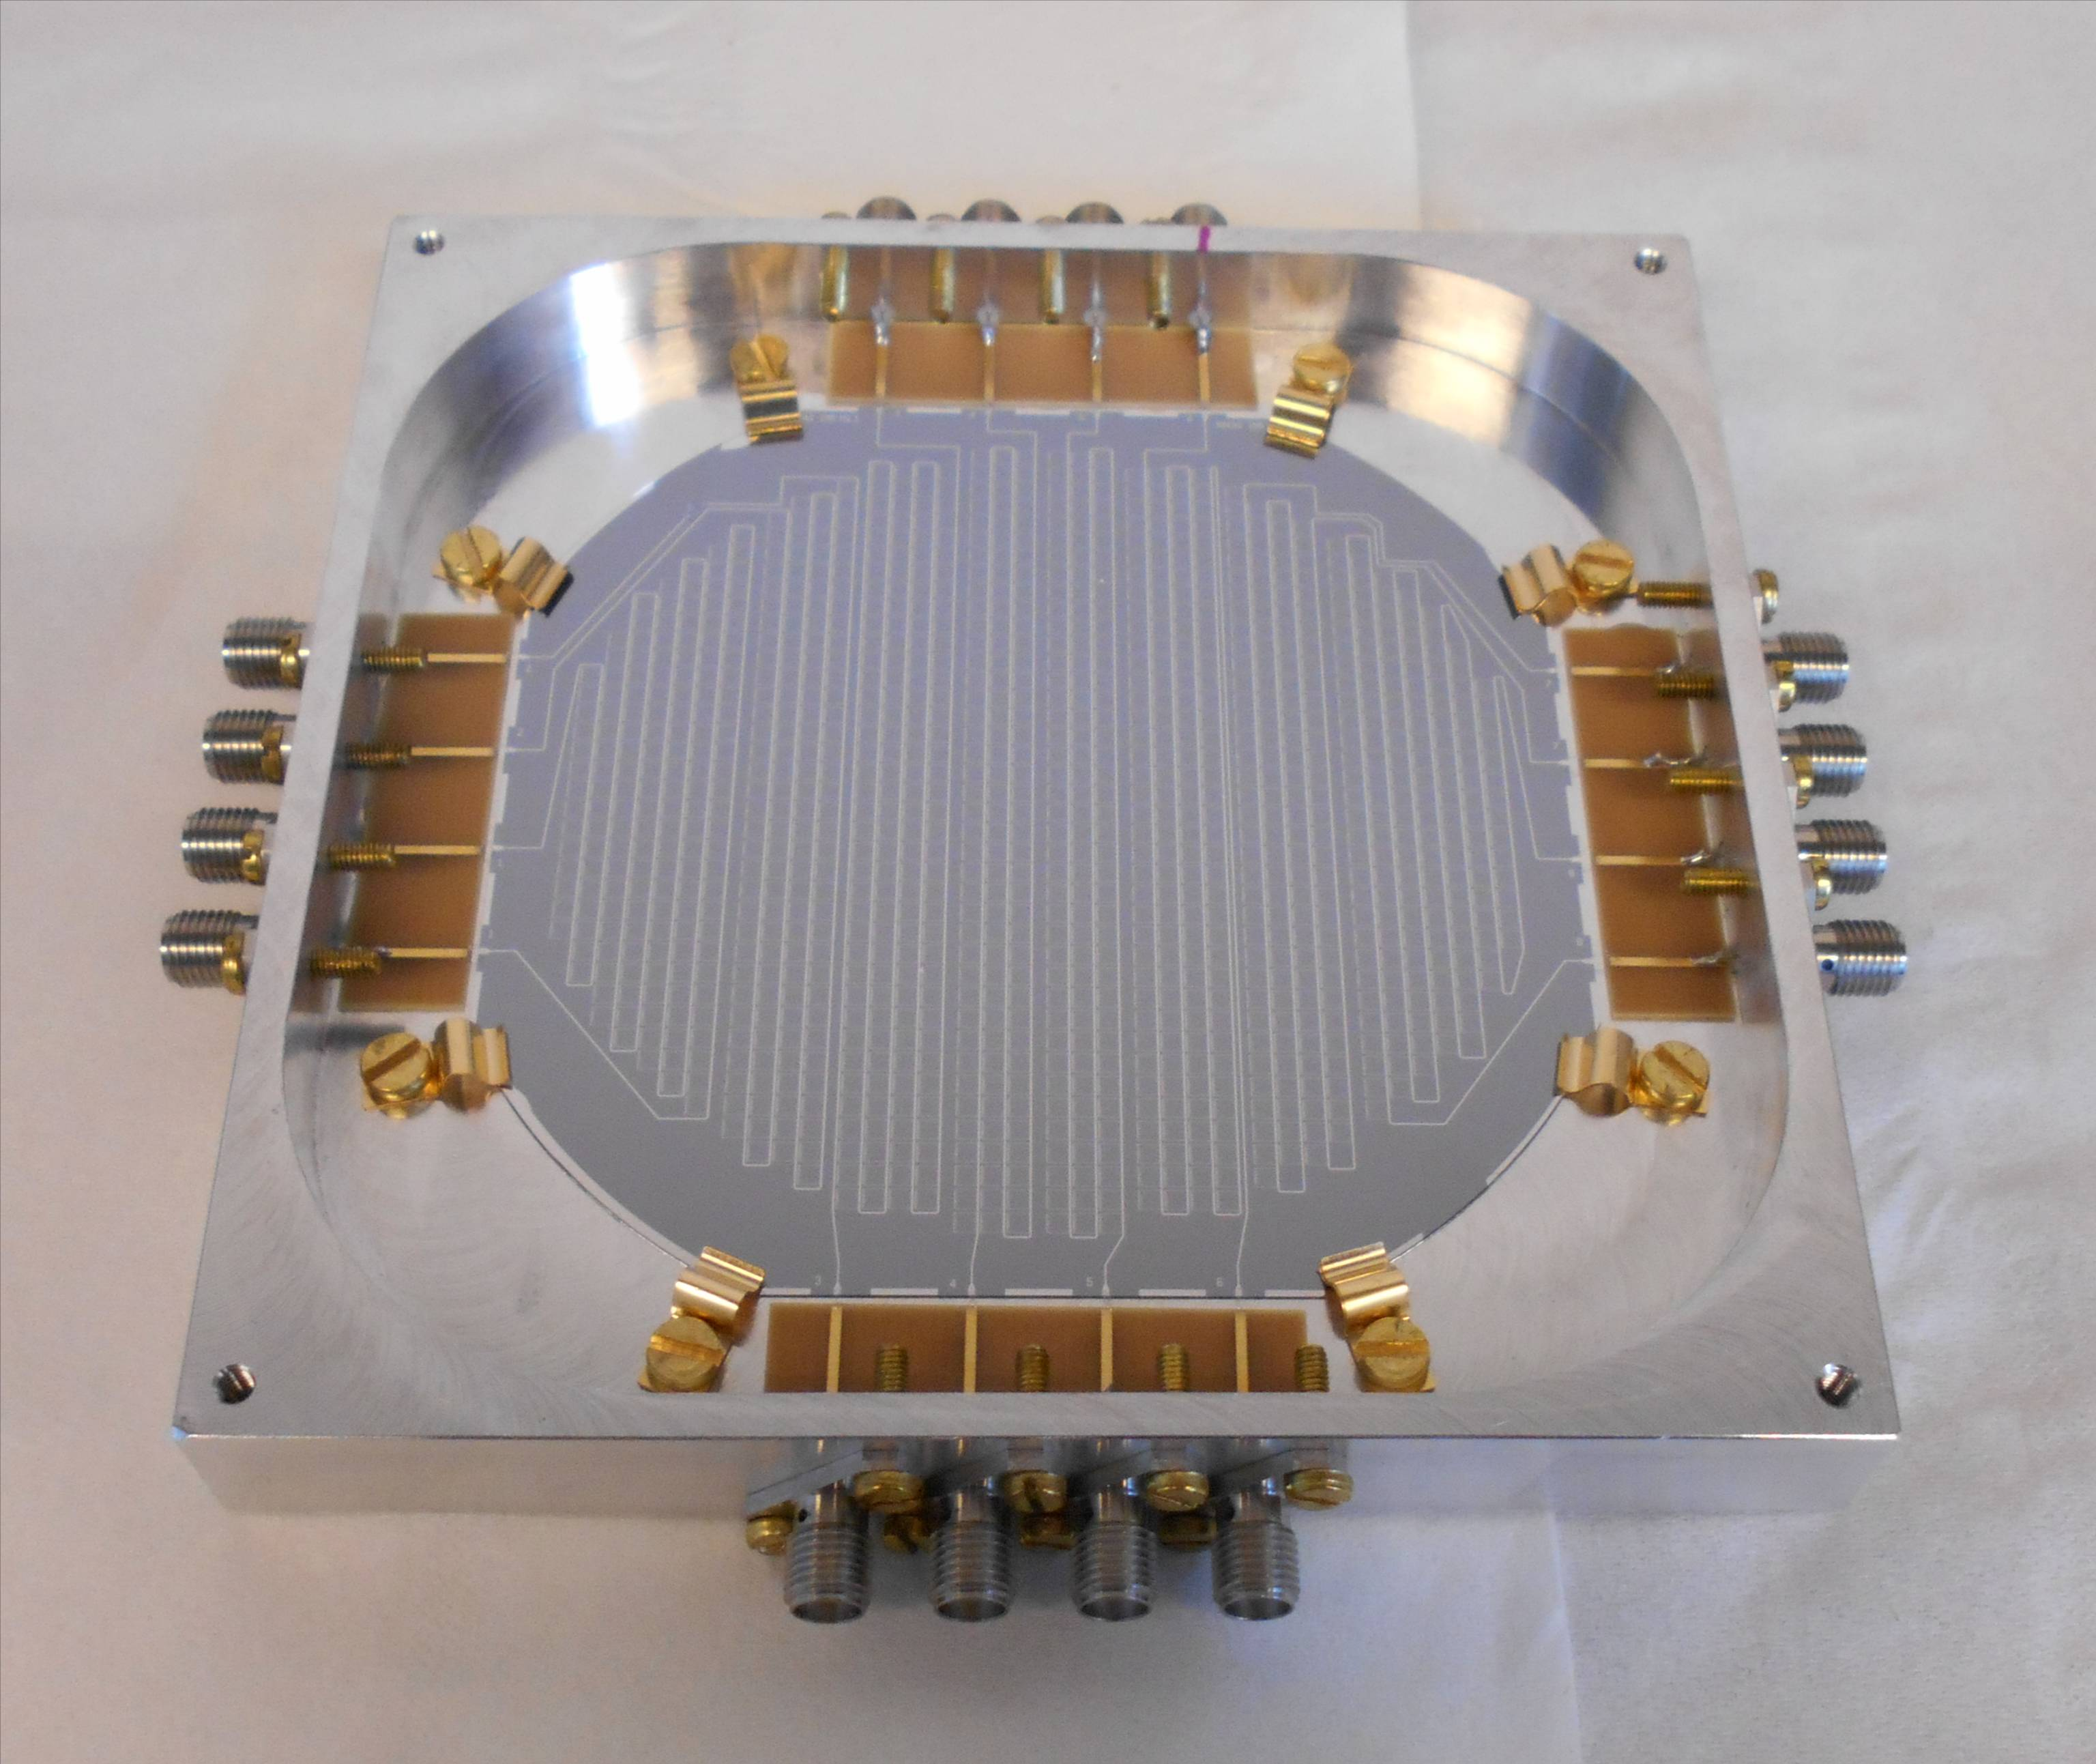
\includegraphics[clip, width=0.75\linewidth]{Figures/NIKA2/1mm_array.jpg}    
  \end{minipage}
  \hfill
  \begin{minipage}[c]{0.50\linewidth}
    \centering
     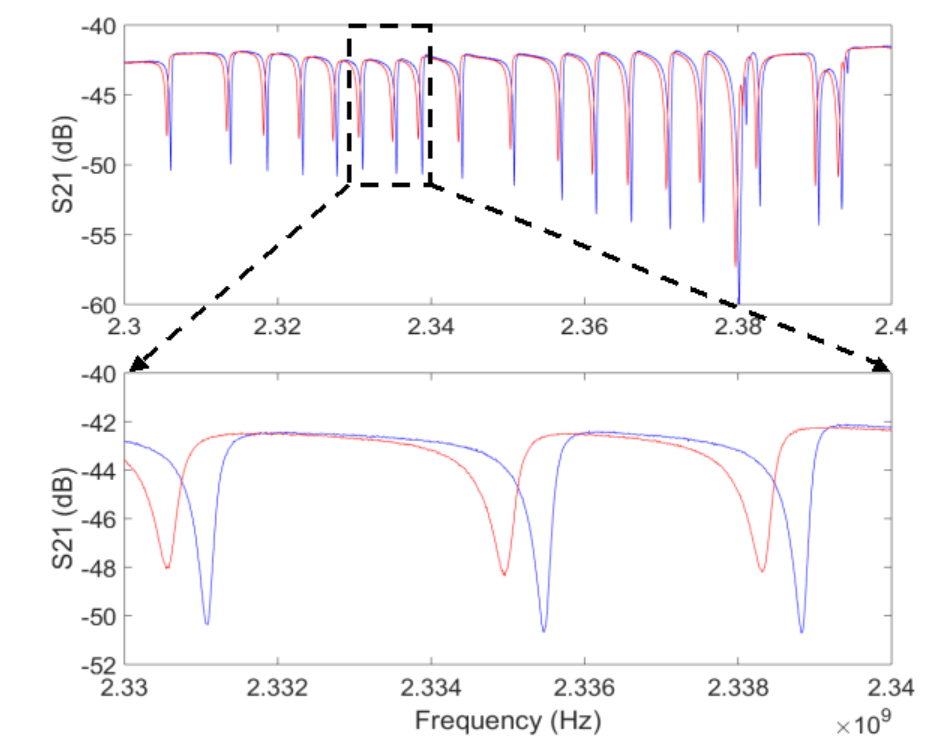
\includegraphics[clip, width=\linewidth]{Figures/NIKA2/260GHz-H_sky.png}
  \end{minipage}
  \caption{Les lignes de base et les données brutes. A gauche, une
    photo d'une des matrices à 1\,mm dans son support. On distingue
    les (8) lignes de base qui connectent chacun des (1140) KID, ainsi
    que les connecteurs d'entrée et de sortie de l'électronique
    froide. A droite est présenté un exemple de mesures des fréquence
    de résonance des KID effectuées en laboratoire. La figure du haut
    montre la fonction de transfert (paramètre de transmission $S_{21}$)
    mesurée à la sortie de l'une des lignes de base dans la bande à
    1\,mm, en effectuant un balayage en fréquence. La figure du bas
    présente un zoom isolant trois courbes de résonance typique. Sur
    les deux figures, les courbes bleues correspondent à la
    transmission des KID illuminés par un fond refroidi à 80\,K,
    tandis que les courbes rouges correspondent à une illumination à
    température ambiante (300\,K). Pour chacun des KID, la forme de la
    transmission varie et le minimum de transmission se décale en
    fréquence en fonction de la lumière reçue. Ces mesures sont
    utilisées pour estimer une réponse moyenne des KID à la
    température du \og ciel \fg dans~\citet{Adam2018}.}
  \label{fig:ma_fig}  
\end{figure}
 
Chaque bloc d'environ 150 KID est connecté à une même ligne de base
(câble co-axe) assurant la transmission du signal d'excitation en
entrée des détecteurs et la lecture du signal transmis en sortie des
détecteurs. La ligne d'excitation (entrée) et la ligne de lecture
(sortie) sont connectées directement sur la plaque de silicone à 150~mK
supportant les KID, au moyen de connecteurs dédiés (subminiature
version A, SMA). Le signal de sortie est dirigé vers un amplificateur
cryogénique à bas bruit (Low-noise amplificateur, LNA) spécialement
conçu pour NIKA2 (Observatoire \emph{Yebes} et entreprise \emph{TTI
  Norte} en Espagne). La matrice A2 est connectée à quatre lignes de
base tandis que huit lignes de bases équipent chacune des matrices à
1~mm, A1 et A3. Les connecteurs (SMA) d'entrée et de sortie pour l'une
des matrices à 1~mm sont visibles à la
figure~\ref{fig:ma_fig}. Cet ensemble, comprenant les connecteurs SMA,
le câbles d'excitation et de lecture et les amplificateurs LNA forme
l'électronique froide, placée à l'intérieur du cryostat et faisant le
lien entre l'étage à 150~mK et la cabine du télescope (300~K).

Ensuite la production du signal d'excitation, la lecture des signaux
de sortie et les conversions entre signaux analogiques et digitales
pour les 2 900 détecteurs sont réalisés par une électrique de lecture
dédiée, développée pour NIKA et NIKA2 au LPSC à Grenoble. Cette
électronique, appelée \emph{New Iram Kid Electronic in Advanced
  Mezzanine Aard format} (NIKEL-AMC), se compose de 20 cartes
électroniques, chacune couvrant une bande de fréquence de 500~MHz et traitant
les signaux d'entrée et de sortie de 150 KID. Dans chaque bande de
500~MHz, le signal d'excitation est produit au moyen de cinq
convertisseurs digital-vers-analogique (DAC) couvrant chacun 100~MHz,
créant ainsi une sous-bande commune à une trentaine de KID.   
Les différentes cartes électroniques sont synchronisées entre elles et
avec le télescope de 30-m par un signal à un pulse par seconde (PPS)
fourni par le GPS du système de contrôle du télescope. Une description
détaillée de l'électronique de lecture de NIKA2 est donnée dans
\citet{Bourrion2012, Bourrion2016}.



\subsection{L'acquisition des données brutes}
\label{se:rawdata}

La photométrie avec des KID repose sur la mesure des variations de
leur fréquences de résonance, qui varient proportionnellement à la
puissance optique reçue (voir Sect.~\ref{se:kid}). Les performances
des KID, utilisés comme détecteurs dans le domaine millimétrique, ont
été décrites théoriquement dans \citet{Swenson2010} et testées en
laboratoire avec les détecteurs de NIKA~\citep{Monfardini2014JLTP}. 

La mesure de la fréquence de résonance des KID se fait via la mesure
de la fonction de transfert entre le signal d'excitation envoyé en
entrée de la ligne de base et le signal transmis par les KIDs en
sortie. Un exemple de mesure de la fonction de transfert d'une série
de KID connectés à une même ligne de base, en fonction de la fréquence
du signal d'excitation est montré à la figure~\ref{fig:ma_fig}. La
résonance de chaque KID est repérées par un pic d'absorption du signal
d'entrée. Ainsi, chaque KID est associé à une fréquence
$f_{\rm{tone}}$, correspondant à sa fréquence de résonance pour une
puissance optique incidente de référence (définie, par exemple, en
occultant la fenêtre d'entrée du cryostat).

Les variations de fréquence de résonance des KID dues à la lumière
incidente $\Delta f$ se traduisent par des variations de leur fonction
de transfert complexe. Celle-ci est caractérisée par deux
quantités : une composante variant en phase avec le signal d'entrée,
notée $I$ (\emph{In-phase}) et une composante variant en quadrature,
notée $Q$ (\emph{in-Quadrature}). Il s'agit alors de relier les
quantités mesurées via le système d'acquisition de données, qui sont
les composantes de la fonction de transfert $I$ et $Q$ et ses
variations $\Delta I$ et $\Delta Q$, aux variations de fréquence de
résonance $\Delta f$. Pour cela, une méthode originale a
été développée pour NIKA et NIKA2, et est décrite dans
\citet{Calvo2013}.
Le signal d'excitation d'entrée est modulé à une fréquence fixée $df$,
où $df$ est très petit devant la largeur de la résonance. La mesure de
la variation de la fonction de transfert induite par ce décalage en
fréquence connu, $dI$ et $dQ$, nous permet de calibrer la relation
entre $\Delta I$ et $\Delta Q$ et $\Delta f$. Il est alors possible de
définir une quantité directement proportionnelle à $\Delta f$. Cette quantité,
appelée \emph{RF\_dIdQ}, est définie comme la projection dans le plan
($I$, $Q$) du vecteur ($\Delta I$, $\Delta Q$) sur le vecteur ($dI$,
$dQ$). Cette quantité, proportionnelle à $\Delta f$ pour chaque KID,
constitue le signal ordonné en temps (\emph{Time Ordered Information},
TOI) des détecteurs. 
Ainsi, à partir des données brutes fournies par le système
d'acquisition, comprenant les quantités $I$, $Q$, $\Delta I$ et
$\Delta Q$, échantillonnées à $f_{\rm{sam}} = 23,4~\rm{Hz}$, pour
chaque KID, les TOI des KIDs sont construites. \'Etant
proportionnelles aux variations de fréquence de résonance, elles
s'expriment en Hz.

% ajouter un paragraphe sur le tuning ??
Finalement, pour maximiser la sensibilité des KID, le signal d'excitation
$f_{\rm{tone}}$ doit être proche de la fréquence de résonance. Or
celle-ci dépend du signal astrophysique mais aussi du bruit, dominé
par l'émission thermique de l'atmosphère. Le signal d'excitation doit
donc être adapté en temps réel, aux variations du rayonnement de fond 
d'origine atmosphérique, qui dépendent des fluctuations d'opacité de
l'atmosphère et de l'épaisseur d'atmosphère traversée sur la ligne de
visée, elle-même déterminée par l'élévation à laquelle se font les
observations. Pour cela, une procédure d'ajustement des
$f_{\rm{tone}}$, appelée {\tt tuning}, a été inclue à l'acquisition
de données~\citep{Adam2018}. Un {\tt tuning} est automatiquement
réalisé lorsque le télescope pointe vers une nouvelle source et au
début de chaque observation. Cette optimisation, qui ne prend que deux
secondes, permet de conserver une bonne sensibilité même dans des
conditions d'observation défavorables (forte opacité, instabilité de
l'atmosphère, observations à fort gradient d'élévation).



\subsection{Caractérisation en laboratoire}
\label{se:bandpass}

Une intense phase de caractérisation en laboratoire à l'Institut Néel
a précédée l'installation au télescope de 30-m de NIKA2, comme du
prédécesseur NIKA. Cette phase, qui a aussi mobilisée les équipes de
l'IPAG, l'IRAM et du LPSC a été cruciale pour l'élaboration du
dispositif instrumental final. En outre, deux bancs test originaux ont
été développés : un simulateur de ciel et un interféromètre
pour les mesures de bandes passantes.

Le simulateur de ciel, consistant en une bille mobile placée devant un
fond froid illuminant le plan focal via une lentille, est détaillé dans
\citet{Catalano2014, Monfardini2011_NIKA}. L'analyse des données issues de
"l'observation'' du simulateur de ciel a permis de tester les
performances des KID, d'optimiser les sous-systèmes instrumentaux, de
mettre en place et de tester le système d'acquisition et les outils de
traitement de données. Cette série de tests et les principaux
résultats obtenus pour NIKA2 sont résumés dans \citet{Adam2018}.


La caractérisation des bandes passantes de NIKA2 s'est effectuée au
moyen d'un interféromètre de Martin-Puplett (IMP) conçu à l'Institut
Néel~\citep{Durand2007_these}. L'IMP, couplé à une source de référence de
spectre de Rayleigh-Jeans, fournit un signal optique finement
sélectionné en fréquence. Ce signal dirigé à l'entrée du cryostat
vient illuminer le plan focal après avoir traversé le système optique
froid, permettant une mesure de la réponse spectrale en
transmission. Les bandes passantes pour chacune des trois matrices de
détecteurs sont présentées à la
figure~\ref{fig:bandpass}. L'incertitude sur ces mesures permises
par le IMP est estimée meilleure que $1\%$. Les bandes
passantes de NIKA2 sont comparées à la transmission de l'atmosphère
pour deux contenus en vapeur d'eau (définis par la hauteur d'eau
précipitable ou \emph{precipitable water vapour}, pwv). Comme discuté
au paragraphe~\ref{se:optics}, la bande passante de A2 rempli bien la
fenêtre de transmission de l'atmosphère, tandis que les bandes
passantes de A1 et A3 tendent vers zéro vers 300~GHz pour limiter le
bruit atmosphérique dans les conditions d'observation moyenne à
médiocre.

\begin{figure}[!thbp] 
\begin{center}
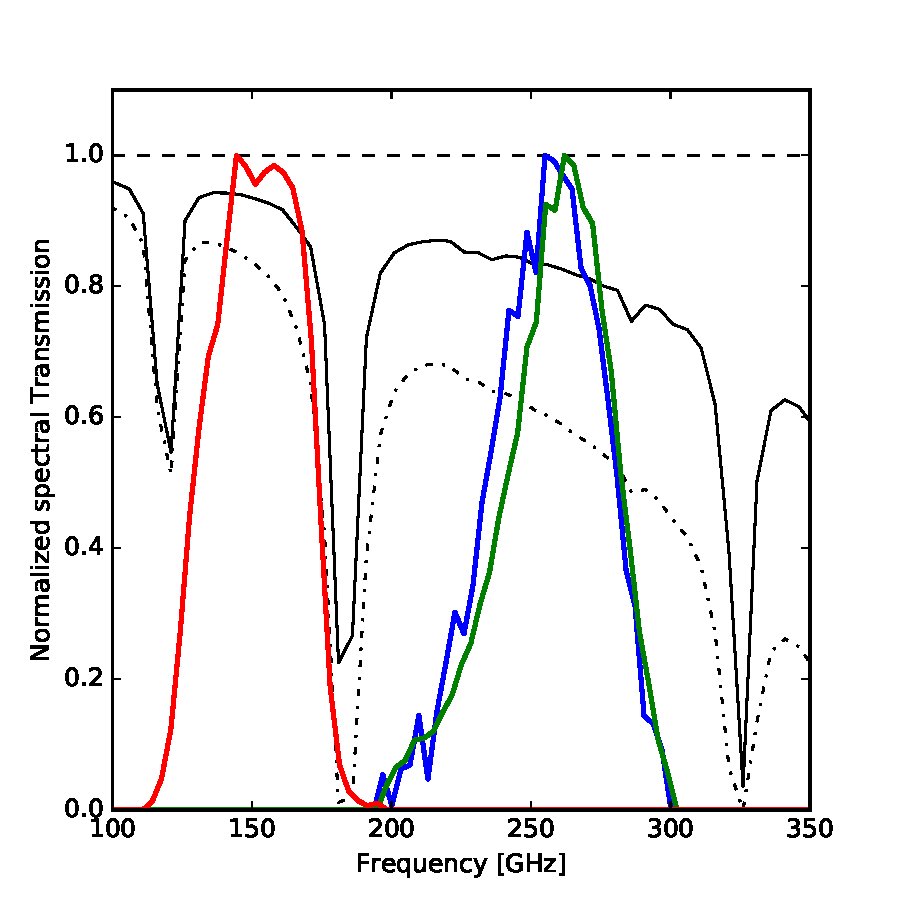
\includegraphics[clip,width=0.5\textwidth]{Figures/NIKA2/atm_transmission.pdf}
\caption[Les bandes passantes]{Les bandes passantes de NIKA2. La
  transmission spectrale de la matrice à 150\,GHz (A2 en rouge) et des
  deux matrices à 260\,GHz (A1, en bleu, et A3, en vert) est tracée en
  fonction de la fréquence. Ces courbes ont été mesurées au
  laboratoire dans un cryostat équipé de l'optique froide de NIKA2,
  incluant la première lame dichroïque installée (qui a été remplacée
  en 2016). Pour comparaison, la transmission de l'atmosphère,
  calculée à partir du modèle ATM\citep{Pardo2002}~, est également
  montrée pour deux valeurs de la hauteur d'eau précipitable (pwv) contenue
  dans l'atmosphère. La courbe en trait plein correspond à 2\,mm de
  pwv (bonnes conditions atmosphériques de semestres d'hiver), tandis que la courbe
  en trait discontinu correspond à 6\,mm de pwv (conditions moyennes
  d'observation de semestres d'été).} 
 \label{fig:bandpass}
\end{center}
\end{figure}

%%%%%%%%%%%%%%%%%%%%%%%%%%%%%%%%%%%%%%%%%%%%%%%%%%%%%%%%%%%%%%%%%%%%%%%
%
%
%
%
%             SECTION : OBSERVATIONS
%
%
%
%%%%%%%%%%%%%%%%%%%%%%%%%%%%%%%%%%%%%%%%%%%%%%%%%%%%%%%%%%%%%%%%%%%%%%%
\section{Observations au télescope}
\label{se:observations}

%\subsection{Le télescope de 30-m de l'IRAM}
Le télescope de 30-m de l'IRAM~\footnote{Science User's web pages: {\tt
  http://iram-institute.org/EN/content-page-55-7-55-0-0-0.html}}, en
opération depuis 1985, se situe à Pico Veleta
à 2870 mètres d'altitude, dans la Sierra Nevada espagnole. Ce site a
été choisi pour sa latitude suffisamment basse (37 degré nord) pour
observer des sources jusqu'à une déclinaison d'environ -30
degrés sur le ciel et ses conditions météorologiques (sécheresse et
altitude). Le télescope est de type Nasmyth-Cassegrain, constitué d'un
miroir primaire parabolique équipé d'une monture
altazimutale~\citep{Baars1987}. Les instruments sont placés dans la
cabine \emph{Nasmyth}, située sous le miroir primaire et liée à
celui-ci en azimuth. La structure qui soutient le miroir primaire est conçue
suivant le principe homologique : elle minimise l'impact des
déformations du miroir sous l'effet de sont propre poids en le
contraignant a garder une forme parabolique à toutes les
élévations. De plus, l'ensemble du miroir primaire est thermalisé afin
de limiter les déformations dues aux variations de la température
extérieure~\citep{Baars1988}. Cette conception permet au télescope de
30-m d'offrir une résolution angulaire jusqu'à 10 arc-secondes et une
précision de pointage meilleure que 3 arc-secondes~\citep{Greve1996}.  


Le télescope de 30-m de l'IRAM est un observatoire ouvert à la
communauté scientifique. Des campagnes d'observations regroupant un
ensemble de projets scientifiques sélectionnés (\emph{observation
  pool}) sont organisées durant les semestres ``d'été''
(septembre à décembre) et "d'hiver'' (janvier à juin). Pour les
observations avec NIKA2, plusieurs de ces campagnes (de trois à cinq),
d'une durée d'une semaine, sont planifiées chaque semestre. Les
observations s'effectuent à partir de la salle de contrôle du 30-m en
passant une série d'instructions au système de contrôle du télescope
(\emph{New System Control}, NSC) concernant le pointage, le focus, et
la stratégie de balayage (\emph{scan}).
Pour la plupart des observations avec NIKA2, celle-ci
consiste à balayer continument le ciel dans les deux directions
suivant une coordonnées (azimuth, élévation, ascension droite,
déclinaison), tandis que la coordonnée perpendiculaire (élévation, azimuth,
déclinaison, ascension droite) est incrémentée d'un petit pas à chaque
changement de direction. Cette stratégie de balayage est appelée
\emph{On-the-Fly} (OTF) \emph{scan}. Un balayage continu dans une
direction est un \emph{subscan}. L'ensemble du scan couvre une zone de
ciel formant un rectangle (ou un parallélogramme, un angle pouvant
être défini pour décaler le début de chaque subscan) dans le système
de coordonnées choisi. Plusieurs types de scans ont été optimisés pour les
observations de NIKA2 et sont utilisés lors des
campagnes techniques (commissioning) et scientifiques. Ils sont
décrits dans les sous-sections suivantes.

\subsection{Focus}
\label{se:focus}

Une session d'observation commence par l'optimisation du focus axial
du télescope, consistant à ajuster la position du miroir secondaire
selon l'axe optique, notée $z$. Pour cela, une procédure d'observation
dédiée a été développée pour NIKA2. Cette procédure consiste à
réaliser une série de cartes d'une source ponctuelle pour cinq
positions $z$ du miroir secondaire. Chacune des cartes est obtenue en
réalisant un petit scan OTF d'une durée d'une minute et couvrant une
zone de $1' \times 5'$ sur le ciel. Sur chacune des cartes, sont estimés
le flux de la source et la taille du lobe au moyenne d'ajustement de
Gaussiennes 2D. Les points de mesure du flux et de la résolution
angulaire sont ajustés par une parabole. Le meilleur focus est défini
comme la valeur qui maximise le flux et la résolution angulaire
mesurés pour les trois matrices de détecteurs.

Cette valeur de focus détermine le meilleur focus au centre du champ
de vue. En effet, étant donné la taille des cartes réalisées, ce sont
les détecteurs situés proches du centre des matrices qui contribuent le
plus à la mesure. Or, le champ de vue est suffisamment étendu (6,5' de
diamètre) pour que la surface de meilleur focus ne soit pas plane mais
légèrement incurvée, de sorte que le meilleur focus au centre du champ
de vue soit sensiblement différent du meilleur focus à la
périphérie. Par conséquence, le focus du télescope peut être optimisé
de sorte de maximiser le nombre de détecteurs proches du meilleur
focus. Pour cela, nous avons mesuré les surfaces focales pour chacune
des matrices de détecteurs, comme discuté dans~\citet{Perotto2019}. La
focalisation optimale des matrices est obtenue en décalant le meilleur
focus central de $-0.2~\rm{mm}$.

Comme les variations de température extérieure et d'illumination du
miroir primaire peuvent affectées le focus, une mesure de focus est
systématiquement réalisée aux levés et couchés du soleil, et ré-itérée
régulièrement durant la journée. 

\subsection{Pointage}
\label{se:pointing}

Le pointage consiste diriger exactement l'axe optique du
télescope vers un point dans le ciel. Le pointage du télescope de 30-m
repose sur un modèle de pointage dont les paramètres sont ajustés
plusieurs fois par an~\citep{Greve1996}. 

Une fois le télescope réglé au focus optimal (Sect.~\ref{se:focus}),
une procédure de correction de pointage est exécutée afin de faire
coïncider exactement le point de référence sur l'axe optique du
télescope avec le détecteur de référence de NIKA2. La plupart des
sources de pointage étant des sources radio (e.g. quasars), le
détecteur de référence est choisi au centre de la matrice A2
(150~GHz). Les corrections de pointage pour NIKA2 sont réalisées à
partir de scans dédiés vers une
source ponctuelle brillante. Un scan de pointage ({\tt pointing})
consiste à balayer la source en effectuant un aller-retour à azimuth
constant, puis à effectuer un second aller-retour à élévation
constante, formant ainsi une croix centrée sur la source et composée
de quatre subscans. La position de la source est mesurée à partir de
chacun des subscans. Les différences entre les deux positions mesurées
suivant chaque coordonnée sont utilisées pour dériver une
correction de pointage en azimuth et en élévation. 
 
\subsection{Skydip}
\label{se:skydip}

Un \emph{skydip} consiste à balayer un grand intervalle d'élévation à
azimuth constant dans le but de mesurer l'opacité de l'atmosphère en
faisant varier la masse d'air traversée sur la ligne de visée. 

Pour NIKA2, la variation de puissance optique reçue par les KID, dues
aux variations de la masse d'air avec l'élévation, est telle le décalage des
fréquences de résonance devient trop important pour le système
d'acquisition de données (voir Sect.~\ref{se:rawdata}). Par
conséquence, les \emph{skydip} de NIKA2 doivent s'effectuer pas-à-pas
par paliers en élévation successifs, au début desquels est réalisé un
{\tt tuning} des KID. Par ailleurs, les \emph{skydip} de NIKA2 ne sont
pas directement utilisés pour mesurer l'opacité instantanée de
l'atmosphère mais pour calibrer la réponse des KID aux variations de
transmission atmosphérique (voir Sect.~\ref{se:opacity}). Un {\tt skydip}
consiste en une série de 11 paliers en élévation placés entre 19 et 65
degrés et régulièrement espacés en masse d'air. Le temps d'intégration
par paliers est de 20 secondes, pour une durée totale du {\tt skydip}
d'environ huit minutes.

\subsection{Beammap}
\label{se:beammap}

Les {\tt beammaps} vers des sources compactes très brillantes sont des
observations critiques pour la calibration de NIKA2. Il s'agit de
longs scans de type OTF définis pour permettre une mesure du lobe de
chaque détecteurs individuellement. Cette contrainte détermine les
paramètres du scan. Le scan est effectué en coordonnées équatoriales
($\az$, $\elev$) à élévation constante afin de minimiser les
variations de la transmission atmosphérique avec la masse d'air. En
coordonnées équatoriales ($\az$, $\elev$), le scan couvre un rectangle
de $13' \times 7.8'$, afin d'assurer que tous
les détecteurs observent complètement la source, même ceux situés
sur les bords des matrices. Un scan plus long dans la direction de
balayage permet une meilleure soustraction de bruit, en assurant un
nombre suffisant de détecteurs pointant loin de la source à chaque
instant. Pour échantillonner le lobe des matrices à 1~mm,
les subscans ne sont séparés que de 4.6'' et la vitesse de balayage
est fixée à 65 secondes par arc-seconde, permettant des mesures
espacées de 2.7'' dans la direction de balayage, soit un
échantillonnage meilleur que le critère de Nyquist. La durée de chaque
subscan est fixée à $12~\rm{s}$, proche de la durée minimale de
$10~\rm{s}$ imposée par le télescope de 30-m. En deçà de cette limite,
le rapport du temps passé par le télescope à changer de direction par
rapport au temps d'observation utile devient prohibitif. L'observation
d'une {\tt beammap} dure environ 25 minutes. 



%%%%%%%%%%%%%%%%%%%%%%%%%%%%%%%%%%%%%%%%%%%%%%%%%%%%%%%%%%%%%%%%%%%%%%%
%
%
%
%
%             SECTION : COMMISSIONING
%
%
%
%%%%%%%%%%%%%%%%%%%%%%%%%%%%%%%%%%%%%%%%%%%%%%%%%%%%%%%%%%%%%%%%%%%%%%%
\section{Commissioning de NIKA2}
\label{se:commissioning}

\subsection{Historique du projet NIKA2 : le précurseur NIKA}
\label{se:nika}

L'aventure de NIKA2 débute avec le développement de l'instrument
précurseur, NIKA, à la fin des années 2000. En octobre 2009, la
première version de NIKA, alors équipé de 69 KID, voit sa première
lumière au télescope de 30-m de l'IRAM~\citep{Monfardini2010_NIKA}. Un
an plus tard, en octobre 2010, une campagne technique est organisée
pour tester NIKA dans une version proche de sa version finale. Il est
alors équipé 356 KID distribués dans deux matrices opérant à 150 et
260~GHz~\citep{Monfardini2011_NIKA}. Je rejoins le projet à l'automne
2011, d'abord pour effectuer les tests en laboratoire, puis pour
participer aux campagnes techniques au télescope de 30-m et à
l'analyse de données. Entre 2011
et 2014, sept campagnes techniques seront organisées. Les excellentes
performances de cet instrument prototype, décrites
dans~\citet{Catalano2014}, justifie l'organisation de trois campagnes
scientifiques au 30-m de l'IRAM sur sélection de projets d'observation
en 2014 et 2015. La calibration et
la livraison des données aux observateurs est alors à la charge de la
collaboration NIKA et est réalisée par les équipes de l'IPAG et du
LPSC. En parallèle, l'instrument NIKA2 est construit et testé sous
la coordination de l'Institut Néel. En janvier 2015, j'intègre
l'équipe c\oe ur (\emph{Core Team}) de la collaboration NIKA-NIKA2. Les
observations avec NIKA ont donné lieu à une série de publications
d'intérêt astrophysique et cosmologique dans les domaines des amas de
galaxies~\citep{Adam2014, Adam2015, Adam2016, Adam2017, Adam2017kSZ,
  Adam2018, Ruppin2017, Romero2018}, de l'émission diffuse
galactique et la formation stellaire~\citep{Bracco2017, Chacon2017,
  Rigby2018} et de la polarisation~\citep{Ritacco2018}.

\subsection{Déroulé du commissioning de NIKA2}
\label{se:historic}

\subsubsection{L'installation au 30-m}
A l'issu des tests en laboratoire, NIKA2 est installée au télescope de
30-m, comme décrit dans~\citet{Adam2018}, et voit sa première lumière,
avec une partie seulement de l'électronique de lecture, en octobre
2015. La première campagne d'observations techniques avec une lecture
des trois matrices au complet est réalisée en janvier 2016.

\subsubsection{Optimisation du dispositif instrumental}
La campagne suivante, appelé \emph{NIKA2 Run 4} (\emph{N2R4}), en mars
2016, est exempte d'incidents techniques et marquée par une météo
favorable. En particulier, les observations effectuées alors,
permettent une mesure précise des surfaces focales des trois matrices
(voir Sect.~\ref{se:focus}) et la mise au jour d'une courbure
inexpliquée de la surface focale de la matrice A2. N'impactant qu'une
des deux bandes de fréquence, cette courbure est attribuée à une
déformation (défaut de planéité) de la lame dichroïque. Une
intervention sur l'instrument est organisée en
septembre 2016, au cours de laquelle est installée une lame dichroïque
utilisant une nouvelle technologie robuste aux
déformations induites par les très basses températures
(Sect.~\ref{se:optics}). De plus, afin d'améliorer la sensibilité de
l'instrument, les lentilles placées immédiatement devant les matrices
sont remplacées par de nouvelles lentilles corruguées pour limiter
les pertes de lumière par réflexion, et la matrice A2 est remplacée
par une nouvelle matrice ayant démontrée une meilleure sensibilité
lors des tests en laboratoire. Par ailleurs, je deviens officiellement
responsable du commissioning et de la caractérisation des performances
en septembre 2016.

\subsubsection{Fin des modifications instrumentales}
Après l'intervention de septembre 2016, les surfaces focales mesurées
sont en accord avec les prédictions issues de simulations optiques pour
les trois matrices, validant ainsi l'absence de déformations de la
nouvelle lame dichroïque. En revanche, les mesures des gains des
détecteurs (\emph{flat field}) révèlent un gradient significatif dans
le champ de vue de l'une des matrices à 1 mm. Il s'agit de la matrice
A1, illuminée par la composante de polarisation transmise par le
polariseur (Sect.~\ref{se:matrices}). Trois origines sont possibles
pour cet effet : un défaut de transmission de l'une des composantes de
polarisation par la lame dichroïque, un défaut de réalisation de la
lentille corruguée placée devant la matrice A1, un désalignement du
faisceau illuminant A1 suite à l'intervention de septembre. En janvier
2017, une nouvelle intervention sur l'instrument est organisée, au
cours de laquelle les lentilles lisses sont re-installées et
l'alignement optique ré-ajusté finement. Les observations techniques
effectuées après l'intervention (durant \emph{N2R8}) révèlent 1) une
amélioration de la forme des lobes des détecteurs de la matrice A1 due
au meilleur alignement optique et 2) un gradient des gains des
détecteurs de A1 inchangé. Par élimination, cette intervention a
confirmé le défaut de transmission de la lame dichroïque. Au vue de
bonnes performances de NIKA2 par ailleurs (voir Chap.~\ref{chap:nika2_resume}),
le dispositif instrumental a été figé.

\subsubsection{Phase finale du commissioning}
En février 2017 a lieu la première campagne technique avec
l'instrument final, le \emph{NIKA2 Run 9} (\emph{N2R9}). Avec pour
objectifs de parachever la phase de commissioning, publier les
résultats du commissioning et caractériser l'instrument, j'ai
constitué une équipe dédiée, la \emph{Commissioning Tiger Team},
réunissant les principaux contributeurs à l'analyse des données parmi
les membres de la collaboration NIKA2. Une dernière campagne technique
a été organisée en avril 2017 (\emph{NIKA2 Run 10} ou \emph{N2R10}),
incluant une phase de vérification scientifique (SVP) de 30
heures. Après un appel à propositions d'observation
au sein de la collaboration, trois projets ont été retenus :
l'observation d'une galaxie proche (M99), d'un amas de galaxie du
\emph{Large Program} SZ (voir Sect.~\ref{se:LP-SZ}), et d'une source
présentant un possible disque de débris (GJ526). En dépit de
conditions météorologique défavorables et d'un sous-système de la
chaine cryogégique dégradé (turbo pompe en fin de vie), cette campagne
a été couronnée de succès, les observations de la SVP donnant lieu à
la première publication scientifique (non-technique) de
NIKA2~\citep{Ruppin2018}. Une première caractérisation de l'instrument,
s'appuyant sur l'analyse des données du N2R9 et N2R10, a été publiée
dans~\citet{Adam2018}.

\subsubsection{Calibration et caractérisation des performances}
La fin de la phase de commissioning a été officialisée en septembre
2017 à l'issue de la revue des performances par l'IRAM. NIKA2 est
alors devenu un instrument à demeure du télescope de 30-m, ouvert à la
communauté scientifique, sous responsabilité de
l'IRAM. Toutefois, une condition a été ajoutée par l'IRAM pour acter
la livraison de l'instrument, stipulant que soit remis un document
détaillant la calibration et les performances de NIKA2.  

La première campagne scientifique de NIKA2, le \emph{NIKA2 Run 12}
(N2R12), a eu lieu en octobre 2017. L'analyse des données dédiées à la
calibration a mis au jour un manque de flux mesuré sur le calibrateur
secondaire le mieux connu (MWC349). En janvier 2018, ce fut la première
campagne d'observation scientifique d'hiver, aussi appelée \emph{NIKA2
Run 14} (N2R14), bénéficiant de conditions d'observation
stables. A partir des données du N2R14, une variation
journalière du lobe de l'instrument (voir Sect.~\ref{se:beam}) a été
mise en évidence. Cet effet, impactant aussi le flux mesuré, est
compatible avec le flux manquant des calibrateurs secondaires observés
au N2R12. Après correction de l'effet du lobe, une variation
résiduelle (15\%) du flux avec l'opacité de l'atmosphère est observée,
indiquant la présence d'un effet systématique. A l'issue d'une intense
phase de tests des effets systématiques, émerge une méthode de
calibration de référence, assurant une bonne stabilité des flux
mesurés : la calibration \emph{baseline}.

\subsubsection{Début de l'exploitation scientifique}
En juillet 2018, notre équipe livre un \emph{pipeline} de calibration
des données de NIKA2 à l'IRAM. Dorénavant, la calibration est prise en
charge par le responsable des observations avec NIKA2 au télescope de
30-m (Bilal Ladjelate). Nous détaillons la méthode de calibration et
compilons les performances de l'instrument dans le document
\emph{commissioning} (130 pages), remis à l'IRAM en décembre 2018. Ces
méthodes et résultats donnent lieu à un article de référence de
la collaboration NIKA2~\citep{Perotto2019}, soumis pour publication en
juillet 2019. Depuis octobre 2017, NIKA2 totalise 18 campagnes
d'observation scientifiques au télescope de 30-m. La première
conférence internationale\footnote{\emph{Millimeter Universe with NIKA2},
  \url{https://lpsc-indico.in2p3.fr/Indico/event/1765/}} dédiée à
l'exploitation scientifique des données de NIKA2 a réuni 75 personnes
en juin 2019 au LPSC. NIKA2 restera en opération au 30-m au
moins jusqu'en 2030.


\subsection{Organisation du travail}

J'ai pris la responsabilité du commissioning de NIKA2 en septembre
2016. Le défi majeur alors était de faire collaborer les équipes de
NIKA2 spécialistes de l'analyse de données avec des KID (IPAG et LPSC)
et les équipes de l'IRAM, à vocation à livrer les données calibrées de
NIKA2 aux observateurs externes, et d'intéresser aux problématiques
d'analyse de données, les équipes ayant construit l'instrument
(e.g. Institut Néel). L'enjeu était critique du à la nécessité de
partager information et expertise entre NIKA2 et l'IRAM d'une part, et
les experts de l'analyse et de l'instrument d'autre part. J'ai donc
repris l'animation de la réunion hebdomadaire de NIKA2, à la suite de
Nicolas Ponthieu (à qui cette tâche délicate incombait depuis deux
ans), avec une approche pro-active pour inciter chaque partie a
participer et présenter des résultats. En outre, j'ai mis en place ou
ré-organisés des outils de travail collaboratifs, dont une série de
pages wiki. Ce wiki comprenait en particulier un espace
\emph{notebook} pour accueillir la description des analyses réalisées
par chacun. Plus de 90 études ont été postées sur cet espace, qui
s'est avéré un outil efficace pour échanger l'information et garder
une trace des résultats obtenus. Ce système de notes internes,
rassemblées dans les pages wiki et discutées en réunion de
collaboration a été crucial pour dépister les problèmes, puis définir
les tests à effectuer lors des campagnes d'observations techniques.

Une fois le dispositif expérimental figé (janvier 2017) et pour mener à bien la phase de commissioning, la difficulté a été de lutter contre la dispersion des efforts et des pistes d'analyse explorées pour concrétiser une caractérisation complète de l'instrument. Dans ce
but, j'ai rassemblé les principaux contributeurs de la collaboration
NIKA2 à l'effort d'analyse de données pour former une équipe dédiée à
la caractérisation de l'instrument, la \emph{Commissioning Tiger
  Team}. Celle-ci a réuni sept chercheurs du LPSC, IPAG,
Service d'astrophysique du CEA et Observatoire de Paris et un
doctorant. Nous avons adopté des méthodes de travail, qui ont été
cruciales pour l'obtention des résultats finaux. Une réunion
hebdomadaires d'une durée maximale de deux heures a été mise en
place. Ensemble, nous avons d'abord identifié les principaux
\emph{challenges} et les points
bloquants, puis nous sommes partagé les tâches dont l'avancement a été
assuré par un suivi des "actions'' attribuées à chacun. Notre travail
s'est structuré en découpant la calibration et la caractérisation des
performances par blocs (donnant sa structure au chapitre~\ref{chap:calib_perf}). Pour
tester la stabilité des données sur plusieurs campagnes, nous avons
défini des méthodes de référence (et partagé les codes
correspondants). Inversement, des jeux de données de référence ont été
définis pour comparer les différentes méthodes développées. Enfin, en
collaboration avec l'IRAM, nous avons défini une liste de
critères de performance de l'instrument à caractériser, comprenant les
pré-requis définis dans le \emph{Mémorandum of Understanding} (MoU),
mais aussi une liste de caractéristiques à tester, émergeant des
études menées sur les données depuis 2016. 

Entre janvier 2017 et décembre 2018, l'essentiel du développement des
méthodes de calibration et d'estimation des performances s'est
effectué au sein de la \emph{Commissioning Tiger Team}. Nos travaux se
sont concrétisés dans plusieurs réalisations : une première
caractérisation des performances décrites dans~\citet{Adam2018}, puis
présentée à la revue des performances de l'IRAM, le développement et
la mise à disposition d'un \emph{pipeline} de calibration des données,
l'écriture du document \emph{Commissioning\&Performance} (130 pages)
accompagnant la livraison de l'instrument à l'IRAM, écriture d'un
article de référence compilant la description des méthodes et des
résultats du commissioning~\citep{Perotto2019}. 



\subsection{Définition d'un jeu de données de référence}
\label{se:scan_selection}

Le développement des méthodes de calibration et la caractérisation
des performances se sont effectuées conjointement au début de
l'exploitation scientifique, alors que quatre campagnes d'observations
étaient organisées par semestre. Afin de cristalliser ce processus, il
est apparu nécessaire au début 2018, de définir un jeu de données de
référence à partir duquel seront testées les méthodes et dérivés les
résultats finaux. Ce jeu de données devait être suffisamment restreint
pour permettre des tests de robustesse extensifs, mais assez étendu
pour couvrir l'ensemble des conditions d'observation rencontrées sur
le site.

Le jeu de données de référence pour la caractérisation des
performances inclut les observations acquises lors de trois campagnes
: N2R9, la première campagne technique avec le dispositif
instrumental final; N2R12, la première campagne scientifique
organisée pendant un semestre d'été; N2R14, la première campagne
scientifique de semestre d'hiver. Ces trois campagnes couvrent un
intervalle de plus d'un an, garantissant la représentativité des
conditions d'observation au 30-m. Chacune des campagnes d'observation
représente un temps d'observation total d'environ 150 heures réparti
en 1300 scans d'observation environ d'une durée comprise entre
deux et 30 minutes.

Ensuite, pour refléter les performances de l'instrument pour une
exploitation scientifique, nous avons défini une sélection des scans
visant à exclure les conditions d'observations extrêmes. Nous avons
adoptés des critères simples et peu contraignants, portant sur l'opacité
atmosphérique au zénith mesurée dans les bandes de fréquence de NIKA2,
$\taunu$ et sur l'élévation des observations, $\elev$. Précisément,
les scans retenus doivent vérifier :
\begin{itemize}
  \item[i)]{$\tau_{A3} < 0.5$, où $\tau_{A_3}$ est $\taunu$ mesuré
    avec la matrice A3, correspondant à une atténuation atmosphérique
    du flux d'un facteur deux à une élévation de $45\degree$;}
  \item[ii)]{$\elev < 20\degree$, afin de limiter l'impact des déformations du lobe
    sous l'effet de la gravité;}
  \item[iii)]{$x\, \taunu < 0.7$, où $x = 1/\sin(\elev)$ représente la
    masse d'air traversée sur la ligne de visée, correspondant à une
    atténuation atmosphérique du flux d'un facteur deux.}
\end{itemize}

Ces critères n'excluent qu'une petite fraction des scans observés lors
des trois campagnes de référence. %{\color{bleu}{ESTIMER CETTE FRACTION ?}}
Par ailleurs, pour des raisons d'instabilités liées à la température
extérieure, qui seront explicitées plus avant à la
Sect.~\ref{se:fwhm_variations}, nous excluons les observations
acquises entre 9\,h et 10\,h UTC, correspondant au lever du Soleil,
ainsi que celles de l'après-midi, entre 15\,h et 22\,h UTC. L'ensemble
de ces critères de sélection définit la sélection \emph{baseline}. 


%----------------------------------------------------------------------------------------
%
%   
%
%----------------------------------------------------------------------------------------
\chapter{Calibration et Performances}
\label{chap:calib_perf}
%\chapter{Calibration et Performances}

%----------------------------------------------------------------------------------------
%
%   DATA REDUCTION
%
%----------------------------------------------------------------------------------------
\section{La chaîne de calibration et d'analyse des données}
\label{se:pipeline}

\subsection{La calibration}
\label{se:overview_calibration}

La calibration consiste à mesurer un ensemble de propriétés et de
paramètres des détecteurs. Elle s'articule en plusieurs étapes, qui
seront détaillées dans les sections suivantes, et qui comprennent:
\begin{itemize}
  \item{La reconstruction du pointage. Cette étape, qui présente
    des spécificités imposées par l'utilisation de matrices de KID,
    consiste à mesurer la position de chaque détecteur dans le plan
    focal par rapport à un point de référence. Cette procédure, aussi
    appelée géométrie, est décrite à la Sect.~\ref{se:fov_geometry}.}
  \item{Sélection et inter-calibration des KID. Une fois le pointage
    de chaque détecteur connu, il est possible de projeter les données
    ordonnées en temps (\emph{Time-Ordered Information}, TOI)} des KIDs
    pour former des cartes. A partir d'une observation de type
    {\tt beammap} (Sect.~\ref{se:beammap}) d'une source ponctuelle
    et brillante, des cartes individuelles de la source, telle qu'elle
    a été observée par chacun des KID, sont réalisées. Cet ensemble
    de cartes nous permet de mesurer le gain de chaque KID, réalisant
    ainsi leur inter-calibration. Nous réalisons également une
    sélection des KID en fonction d'une série de critères de qualité
    mesurés sur les cartes individuelles.
  \item{La calibration de la réponse à la transmission
    atmosphérique. La fréquence de résonance des KID varie
    proportionnellement aux variations de la transmission de
    l'atmosphère (voir Sect.~\ref{se:rawdata}). En calibrant la
    relation entre
    fréquence de résonance et transmission atmosphérique, il est
    possible de mesurer l'opacité de l'atmosphère pour chaque
    observation. Cette étape est détaillée à la
    Sect.~\ref{se:opacity}.}
  \item{La calibration absolue. A partir de la mesure de l'opacité de
    l'atmosphère lors d'une observation, l'atténuation atmosphérique
    instantanée peut être estimée et corrigée, pour obtenir une mesure
    du flux. Une série de mesures du flux d'un calibrateur primaire
    (e.g. Uranus) nous permet d'estimer le coefficient de calibration
    absolue (Sect.~\ref{se:calibration})}
\end{itemize}

A l'issu de ces étapes, les résultats de la calibration sont compilés
dans un fichier unique, rassemblant toutes les informations sur les
KID. Ce fichier, appelé \emph{kidpar}, contient donc les données de
pointage, la sélection, les paramètres de réponse à l'atmosphère et
les coefficients de calibration relative (gain) et absolue de chaque
KID. Le \emph{kidpar}, qui doit être construit à chaque campagne
d'observation, est passé en entrée de la chaîne de traitement de
données développée par la collaboration NIKA2 (coordinateur: Nicolas
Ponthieu).

\subsection{L'analyse des données}
\label{se:overview_pipeline}

La chaîne d'analyse de données, ou \emph{pipeline}, permet de passer
des données brutes, telles qu'elles sont fournies en sortie de
l'acquisition de données (Sect.~\ref{se:rawdata}), à un ensemble de
cartes par matrices et par bandes de fréquence, utilisables pour
l'exploitation scientifique. La calibration elle-même s'appuie en
grande partie sur cet outil. Il s'articule donc avec la calibration en
venant lire et mettre à jour le \emph{kidpar}. Une fois la calibration
réalisée, et concrétisée par la construction du \emph{kidpar} final,
le \emph{pipeline} est utilisé pour la caractérisation des
performances. Une description de ce \emph{pipeline} utilisé à cette
fin est donnée dans~\citet{Perotto2019}. Nous en présentons rapidement
ici les modules principaux :

\subsubsection{Production et masquage des TOI}
Les TOI des KID sont constituées de l'ensemble des mesures de la
variation des fréquences de résonance. Elles sont produites à partir
des données brutes fournies par l'acquisition suivant la méthode
décrite à la Sect.~\ref{se:rawdata}. Ensuite, sont créés des masques
afin de couper les données non-utilisables pour l'exploitation
scientifique. Tout d'abord, sont détectés les impacts de rayons
cosmiques. \'Etant donné les constantes de temps très courtes des
KID, un rayon cosmique n'affecte q'un seul échantillon de données,
qui est alors masqué. Sont également masquées, les TOI des KID exclus
de la sélection de détecteurs réalisée lors de la calibration, et
les TOI des KID bruités, définis comme les KID dont la rms du bruit
est mesurée à 3$\sigma$ au dessus de la rms médiane du bruit des
détecteurs appartenant à la même matrice.

\subsubsection{Production des TOI de pointage} Le système de contrôle du
télescope, avec lequel l'acquisition des données est synchronisée,
nous fournit une TOI de pointage d'un point de référence dans le
plan focal, qui coïncide avec le détecteur de référence après
l'analyse d'un scan de pointage (voir Sect.~\ref{se:pointing}). A
partir des positions relative des détecteurs par rapport à ce point
de référence, telles qu'elles sont stockées dans le \emph{kidpar},
nous produisons une TOI de pointage pour chacun des KID.

\subsubsection{Calibration des TOI} Les TOI brutes, en Hz, sont converties en
Jy/beam en deux étapes. Elles sont d'abord multipliées par les gains
des détecteurs, évalués à opacité atmosphérique nulle, et par le
coefficient de calibration absolue. Ensuite, elles sont corrigées de
l'atténuation de l'atmosphère sur la ligne de visée, modélisée par
$\exp{\left( \taunu \, x(t)\right)}$, où $\taunu$ est l'opacité atmosphérique
mesurée pour le scan d'observation et $x(t)$ la masse d'air
traversée pour l'élévation au temps $t$.

\subsubsection{Soustraction du bruit corrélé}
Le bruit des détecteurs est dominé par plusieurs composantes de bruit
basse-fréquence commun à plusieurs détecteurs. On parle alors de bruit
\emph{corrélé}. Le bruit corrélé inclut le bruit atmosphérique,
dominant, sauf conditions d'observation exceptionnelles, et commun à
tous les KID, et le bruit électronique, commun aux KID connectés à la
même ligne de base de l'électronique de lecture (voir
Sect.~\ref{se:matrices}). Puisqu'il est commun à plusieurs détecteurs,
il est possible d'estimer un bruit corrélé générique, un
\emph{template}, et de le soustraire aux signaux de chaque KID. Ce
processus, appelé la décorrélation du bruit, est une étape critique du
traitement des données. En effet, le résidu de bruit corrélé est l'un
des facteurs limitant la sensibilité des matrices de KID.

La décorrélation du bruit a suscitée le développement d'une série de
méthodes d'analyse dédiées. Des pistes d'amélioration sont encore à
l'étude~\citep{Ponthieu2020}. La méthode la plus simple pour construire
un template de bruit corrélé repose sur le fait que l'atmosphère,
située dans le champ proche, reste la même à chaque instant pour tous
les KID, tandis que la source, en champ lointain, est observée de
façon décalée en temps par des KID différents. Par conséquent, une
moyenne de la TOI de tous les KID préserve le bruit atmosphérique et
diminue le signal astrophysique. Un template de bruit corrélé estimé
de cette manière est un \emph{mode commun}.

Pour la caractérisation des performances, nous avons opté pour une
méthode simple et robuste, bien adaptée au traitement des objets
compacts (qui constituent la vaste majorité de nos sources de
calibration). Cette méthode, appelée \emph{Most Correlated Pixels} (MCP),
inclut deux raffinements par rapport à un simple mode commun. Tout
d'abord, la matrice de corrélation entre les détecteurs (pixels) est
évaluée afin de construire un mode commun pour chaque détecteur à
partir des TOI des KID qui lui sont le plus corrélés. Ensuite, afin de
limiter encore la contribution du signal astrophysique, seuls les KID
n'observant pas la source sont utilisés pour estimer chaque
échantillon de la TOI de bruit corrélé. Ce masquage de la source dans
l'espace temporel induit un filtrage des échelles angulaires plus
grandes que l'extension du masque. Pour l'étude de sources diffuses,
ce filtrage doit être précisément estimé et corrigé pour retrouver
l'émission étendue. En revanche, la décorrélation MCP préserve bien le
signal des sources compactes. 

\subsubsection{Création de cartes} En utilisant les données de
pointages, les TOI calibrées et débruitées de tous les KID valides
d'une même matrice sont projetées tangentiellement dans une grille
régulière sur le ciel pour former une carte de densité de flux par
matrice. La résolution des cartes est choisie suffisamment haute
(typiquement 2'') pour limiter les effets de pixellisation
même en utilisant la méthode des plus proches voisins (\emph{nearest
  grid point}). Pour combiner tous les détecteurs d'une même matrice,
les TOI sont pondérées par l'inverse de la variance du bruit, celle-ci
étant évaluée à partir de la déviation standard des échantillons de
données pris loin de la source. Chaque carte de flux est accompagnée
d'une carte de variance. Celle-ci est inhomogène, dépendant de la
stratégie de balayage. De plus, le résidu de bruit corrélé
basse-fréquence à l'issu de la décorrélation induit une corrélation
des pixels de la carte. Les cartes de variance sont estimées à partir
de la déviation standard de la carte de flux évaluée loin de
la source et de la carte de coups, construite par comptage du
nombre d'échantillons par pixels de la carte. Le bruit corrélé
résiduel est pris en compte en augmentant l'incertitude sur le flux
d'un facteur variant de 1,2 à 1,5 et dont l'évaluation est décrite
dans~\citet{Perotto2019}.\\

Le \emph{pipeline} d'analyse de données, brièvement décrit
ci-dessus, a été développé d'abord pour la phase de
\emph{commissioning} de NIKA2. Il s'appuie sur l'expérience acquise
avec l'analyse des données de NIKA~\citep{Catalano2014,
  Adam2014}. Comme précédemment mentionné, il constitue l'outil de
base pour la caractérisation des
performances~\citep{Adam2018, Perotto2019, Ponthieu2020}, mais il est
aussi actuellement utilisé pour l'exploitation scientifique de
l'ensemble des données de NIKA2 au télescope de
30-m~\citep{Ruppin2018, Ruppin2019c}.  


%----------------------------------------------------------------------------------------
%
%   FOV Geometrie
%
%----------------------------------------------------------------------------------------
\section{La reconstruction du plan focal}
\label{se:fov_geometry}

Dans les matrices de KID, chaque détecteur est repéré par sa fréquence
d'excitation $f_{\rm{tone}}$ (voir Sect.~\ref{se:matrices}). La
première étape de la calibration consiste donc à relier chaque
détecteur à sa position dans le plan focal. Cette
étape, appelée reconstruction du plan focal ou géométrie, est le
préalable à toute production de cartes du ciel à partir de données
issues de KIDs.

\subsection{Caractérisation des KID}
\label{se:KID_pointing}

Pour ce faire, nous utilisons une observation de type {\tt beammap}
(voir Sect.~\ref{se:beammap}) d'une source compact et brillante, telle
Uranus ou le quasar 3C84, nous permettant de construire une carte
individuelle par KID. L'objectif étant d'estimer les données de
pointage nécessaire à l'obtention de cartes, le processus est
nécessairement itératif. A la première étape, les TOI des KIDs sont
projetées en coordonnées \emph{Nasmyth} (attachées à la cabine du
télescope) à partir des données de pointage du point de référence
fournies par le télescope. Pour chaque KID, la source n'apparait pas
au centre de la carte, mais décalée suivant la position du KID par
rapport au point de référence. C'est cette position du KID relative au
point de référence dans le plan focal que nous estimons, au moyen d'une
gaussienne bi-dimensionnelle ajustée à la carte de chaque KID. 

Une fois les positions des KIDs dans le plan focal connues, des cartes
par KID de meilleure qualité peuvent être construites en utilisant le
\emph{pipeline} d'analyse décrit à la Sect.~\ref{se:pipeline}. Ces
cartes peuvent être alors utilisées pour caractériser les propriétés
de chaque KID, leur gain, lobe et niveau de bruit, en particulier. Les
gains sont mesurés en modélisant les cartes par une gaussienne de
largeur fixe, correspondant au choix du système photométrique de
référence (voir Sect.~\ref{se:calibration}). Les lobes sont
caractérisés par les largeurs à mi-hauteur estimées par l'ajustement
d'une gaussienne bi-dimensionnelle. Le niveau de bruit est mesuré dans
les TOI, après avoir masqué les échantillons pris dans un rayon donné
autour de la source. Ces propriétés servent à leur tour de critères de
sélection des KIDs.

Par ailleurs, les KID apparaissent régulièrement espacés dans le plan
focal, reflétant leur positions physiques dans la matrice. Nous
caractérisons l'adéquation entre les positions mesurées dans le plan
focal et les positions attendues par construction. Pour cela, nous
mesurons l'ensemble des transformations linéaires (translations et
rotations) permettant de relier positions mesurées et positions
attendues. Par cette méthode, la distance moyenne séparant les centres
de deux KID voisins est estimée à $9.8''$ dans les matrices A1 et A3
(1\,mm) et $13.3''$ dans la matrice A2 (2\,mm). En utilisant le
diamètre de la pupille d'entrée du télescope $D$ (Sect.~\ref{se:optics}),
ces mesures nous permettent de comparer l'échantillonnage du plan focal
dans les deux bandes de fréquence par rapport à la limite de
diffraction : on trouve un échantillonnage à 1,1 $\lambda/D$ à
260\,GHz et 0,9 $\lambda/D$ à 150\,GHz, conforme aux attentes
(Sect.~\ref{se:matrices}). En plus de la caractérisation fine du plan
focal, cette étude permet une sélection des KID par repérage de ceux
dont la position mesurée est très éloignée de la position attendue.   


\subsection{Sélection des KID}
\label{se:KID_selection}

Bien que tous les KID fonctionnent et mesurent un signal, certains peuvent
être affectés de divers problèmes rendant leur données difficilement
exploitables ou peu informatives. Les principaux problèmes rencontrés
comprennent 1) la diaphonie, plusieurs KID (deux, rarement trois) dont
les signaux interfèrent du fait de fréquences de résonance proches, 2)
le bruit ou la faible sensibilité, généralement dus à un ajustement
sub-optimal de la fréquence d'excitation à la fréquence de résonance
(\emph{tuning}), et plus rarement, l'ellipticité des lobes,
l'instabilité de la position reconstruite dans le plan focal ou les
doublons de KID à signaux identiques. Les détecteurs affectés par ces
problèmes sont identifiés et masqués pour l'exploitation des données
d'une campagne d'observation.

Une sélection des KID est effectuée lors de l'analyse d'une {\tt
  beammap}. Des coupures automatiques peu sévères, basées sur les
distributions de la FWHM, de la sensibilité et de l'ellipticité des
KID sont d'abord appliquées. Ensuite, la sélection est affinée par
inspection visuelle des cartes par KID. Finalement, les KIDs dont la
position mesurée dans le plan focal ne correspond pas à la position
attendue par construction sont exclus. Cette procédure est répétée
sur plusieurs {\tt beammaps} afin de tester la stabilité des KID
sélectionnés. En particulier, nous avons combiné la reconstruction du
plan focal obtenue à partir de dix {\tt beammaps} observées lors des
deux dernières campagnes techniques (voir
Sect.~\ref{se:historic}). Pour chaque détecteur, la position dans le
plan focal et la FWHM du lobe résultent d'une moyenne des mesures
effectuées sur l'ensemble des {\tt beammap}. Cette géométrie moyenne
est montrée à la figure~\ref{fig:avg_fov_color}.

\begin{figure}[!thbp]
\begin{center}
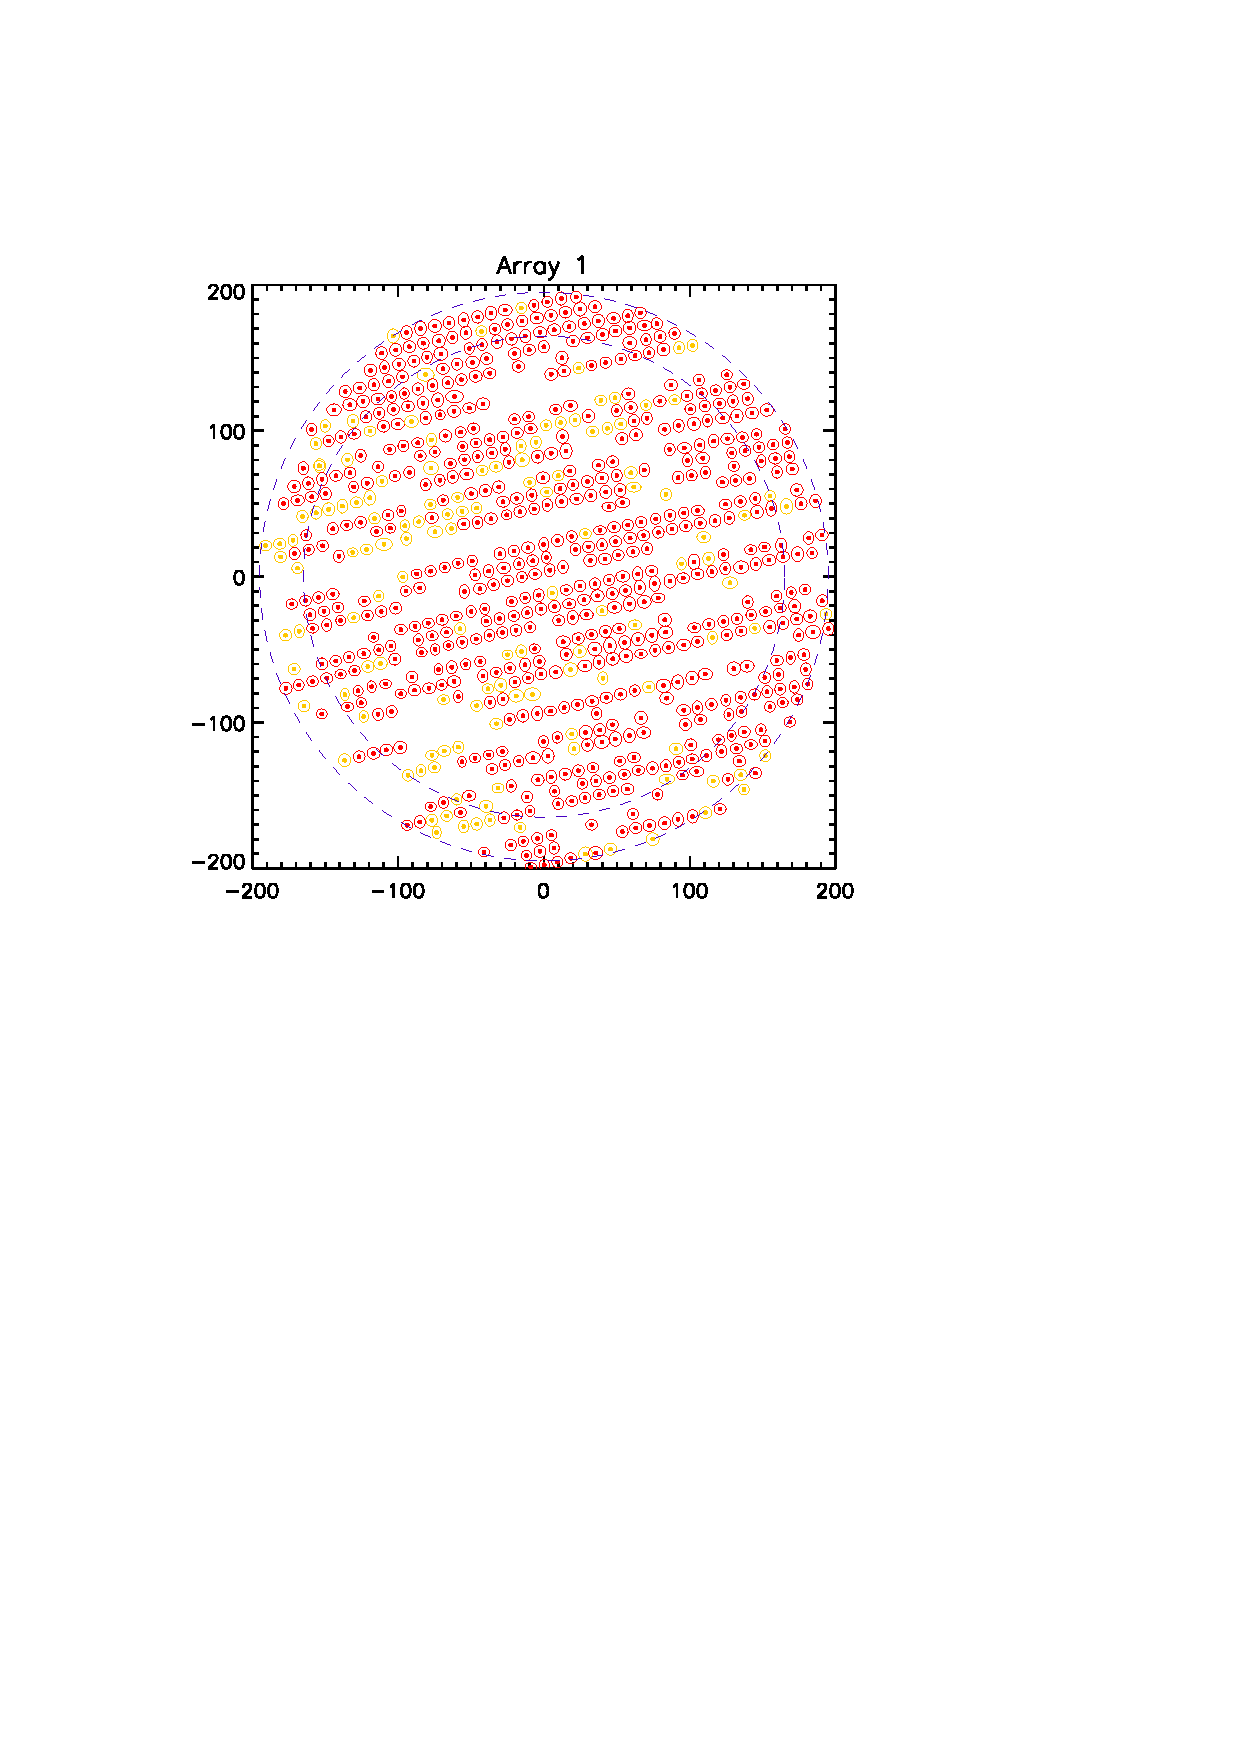
\includegraphics[trim=3cm 14cm 6cm 4cm, clip=true, width=0.32\linewidth]{Figures/NIKA2/A1_fwhm_color_count.pdf}
%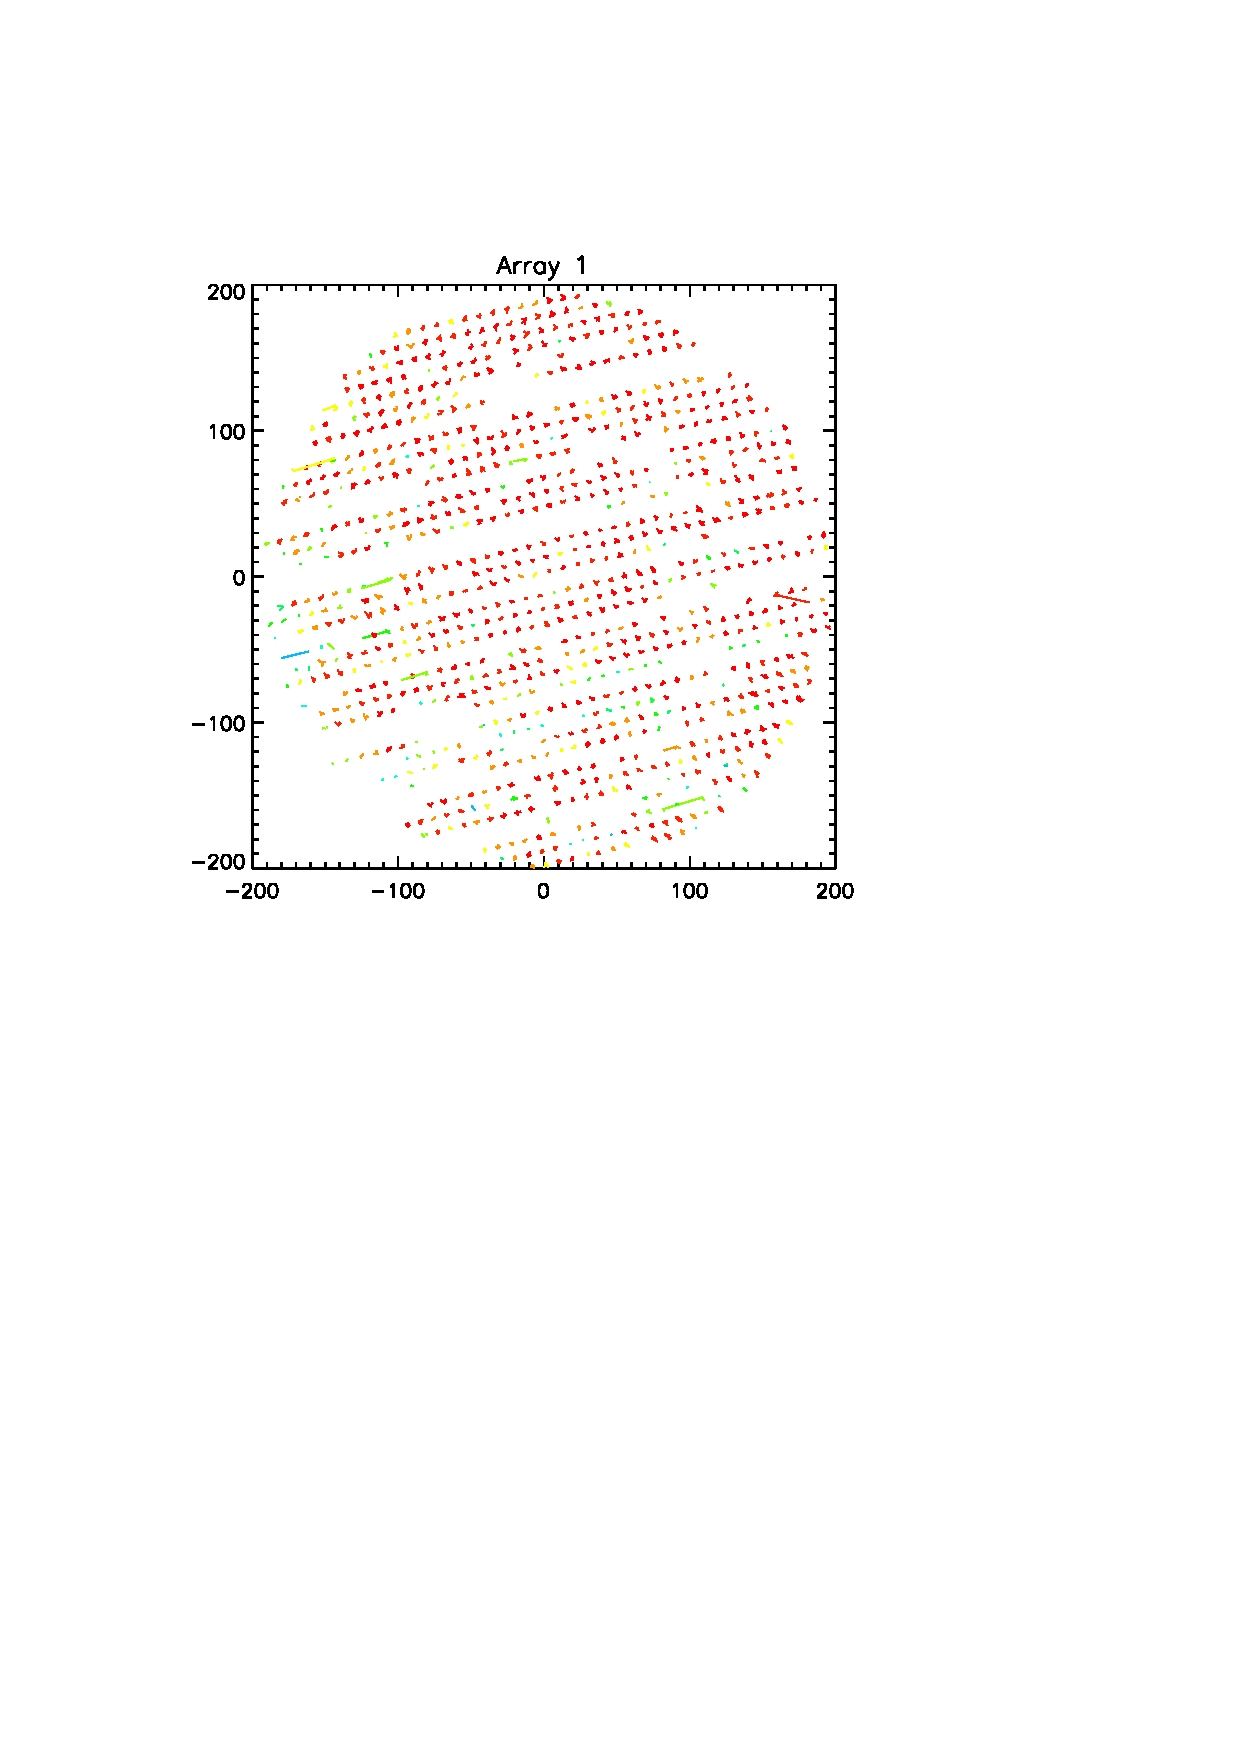
\includegraphics[trim=2cm 14cm 5cm 4cm, clip=true,width=0.45\linewidth]{Figures/A1_positions.pdf}
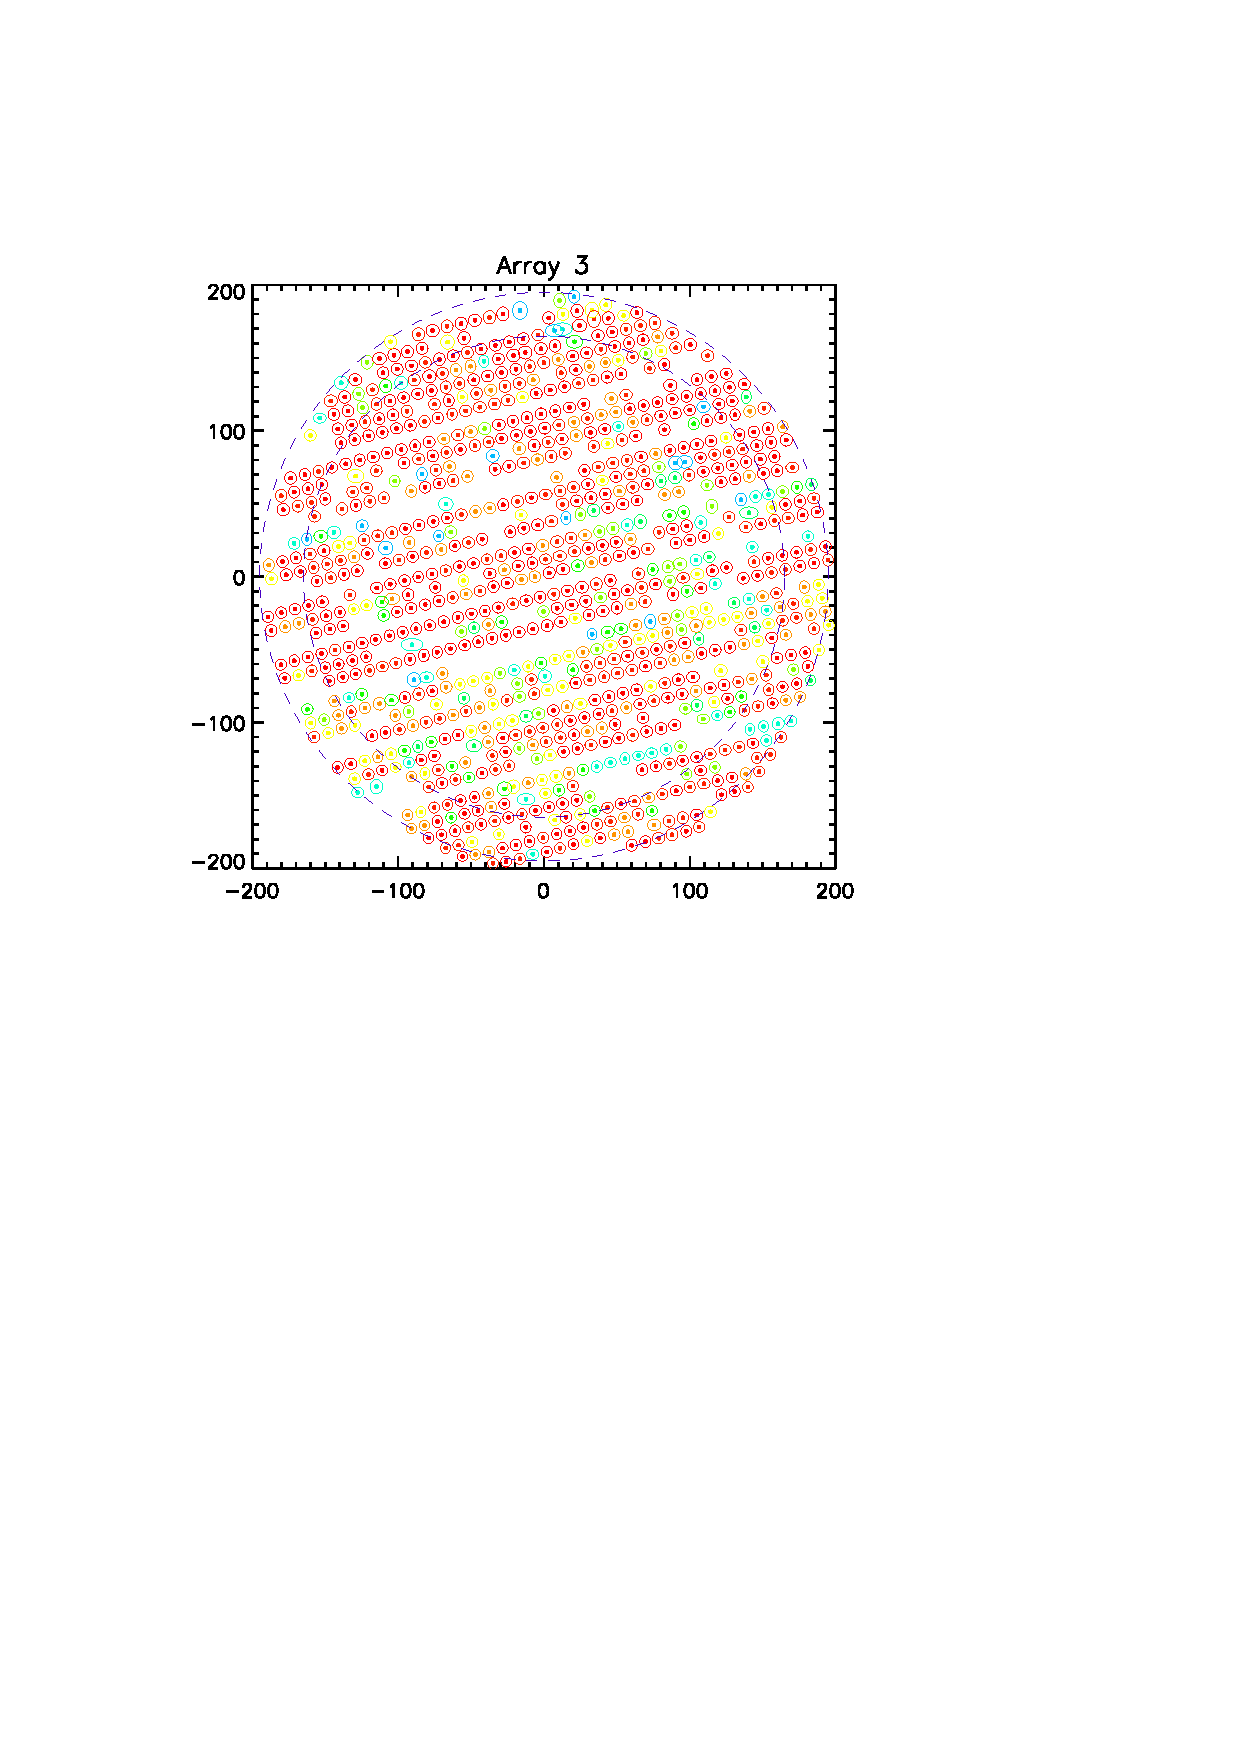
\includegraphics[trim=3cm 14cm 6cm 4cm, clip=true, width=0.32\linewidth]{Figures/NIKA2/A3_fwhm_color_count.pdf}
%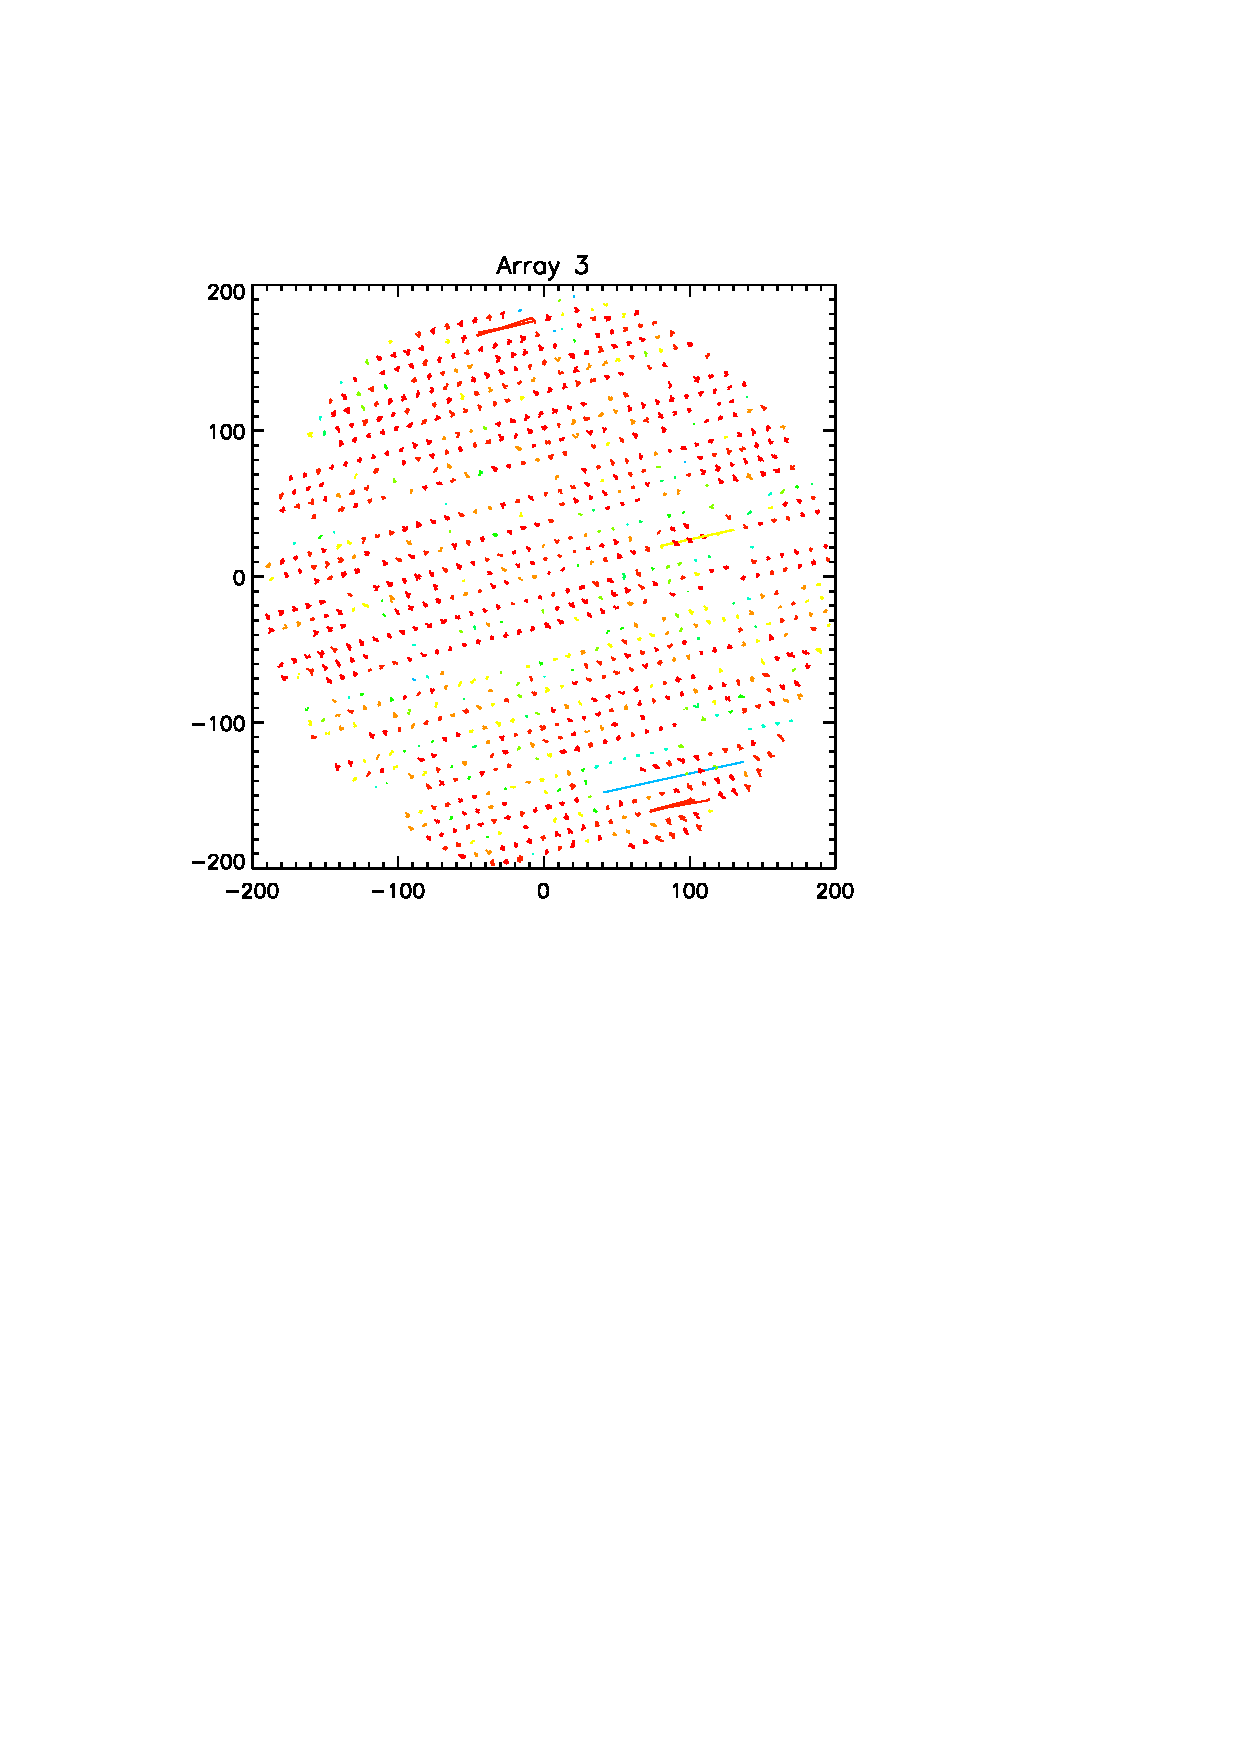
\includegraphics[trim=2cm 14cm 5cm 4cm, clip=true,width=0.45\linewidth]{Figures/A3_positions.pdf}
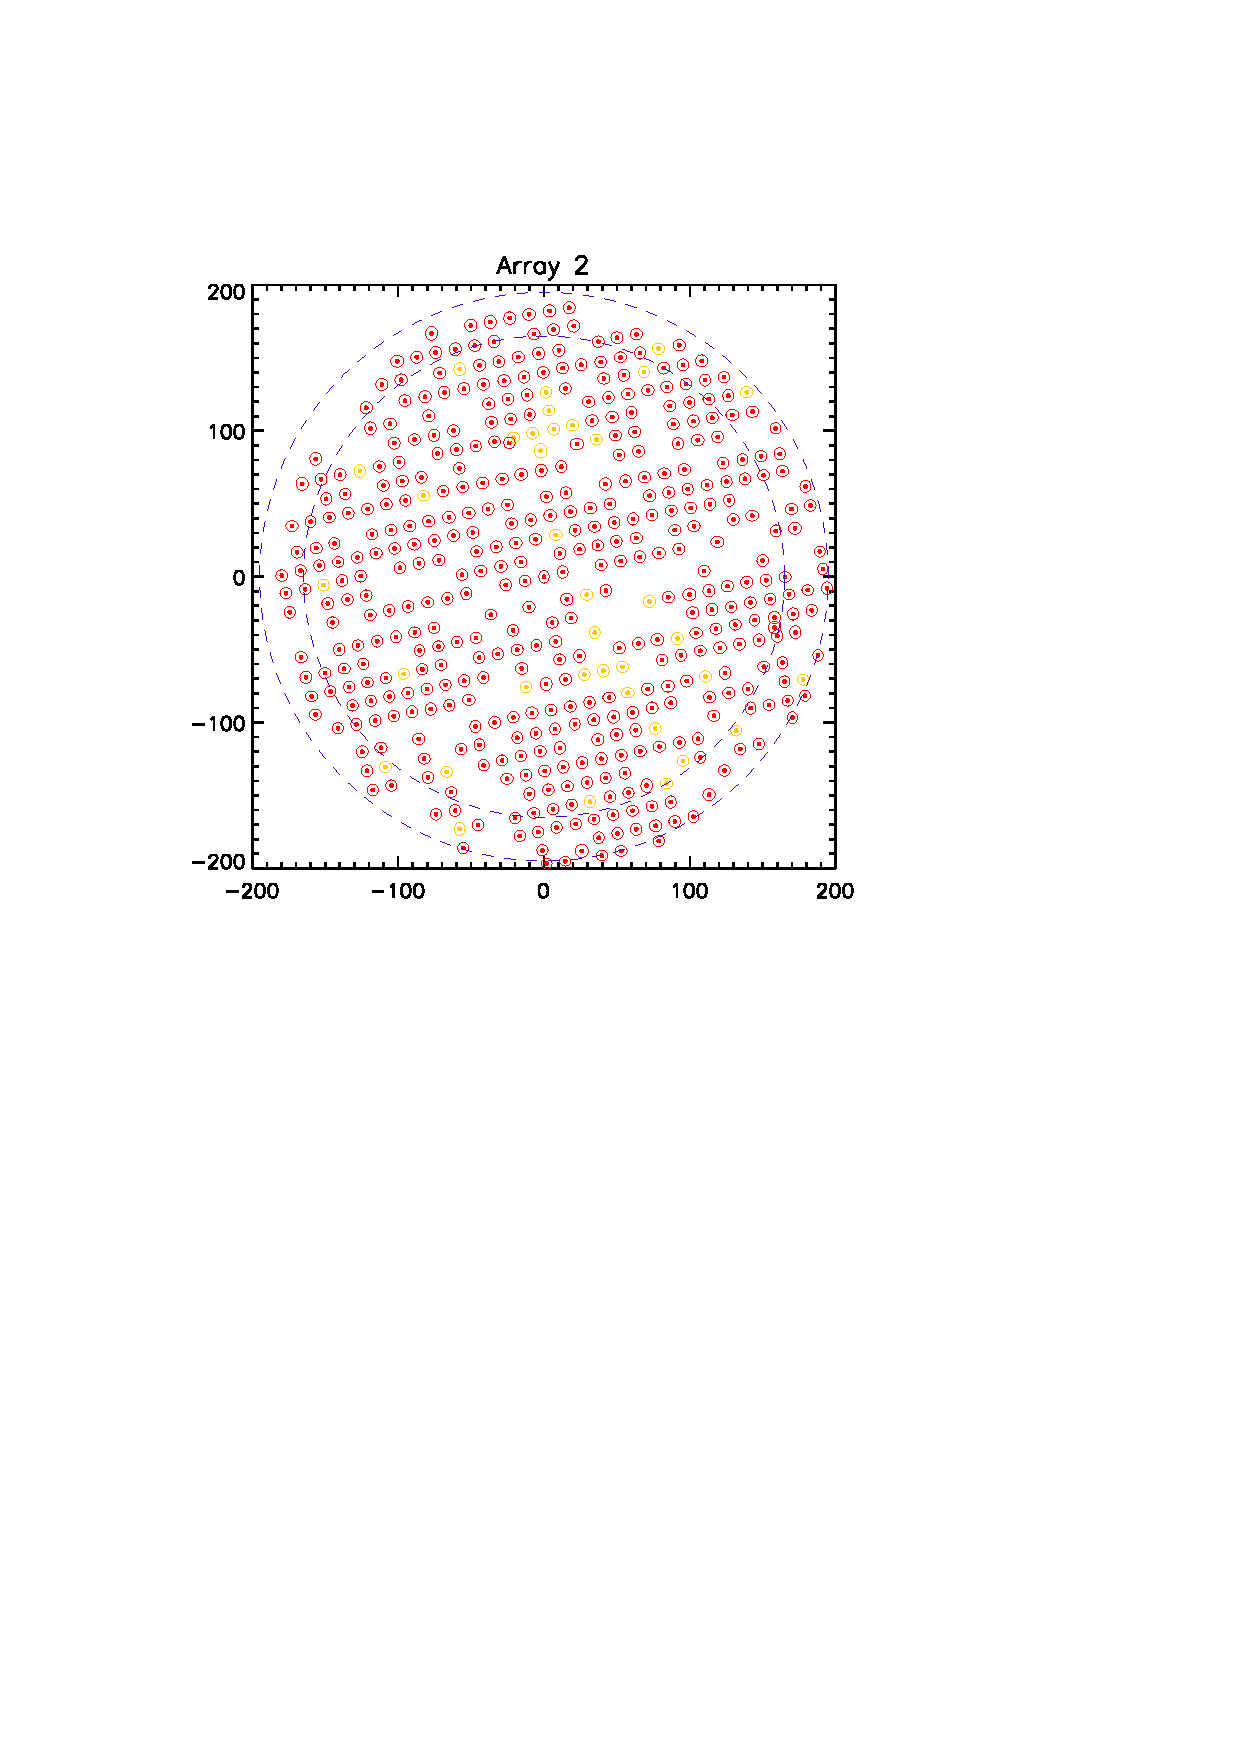
\includegraphics[trim=3cm 14cm 6cm 4cm, clip=true, width=0.32\linewidth]{Figures/NIKA2/A2_fwhm_color_count.pdf}
%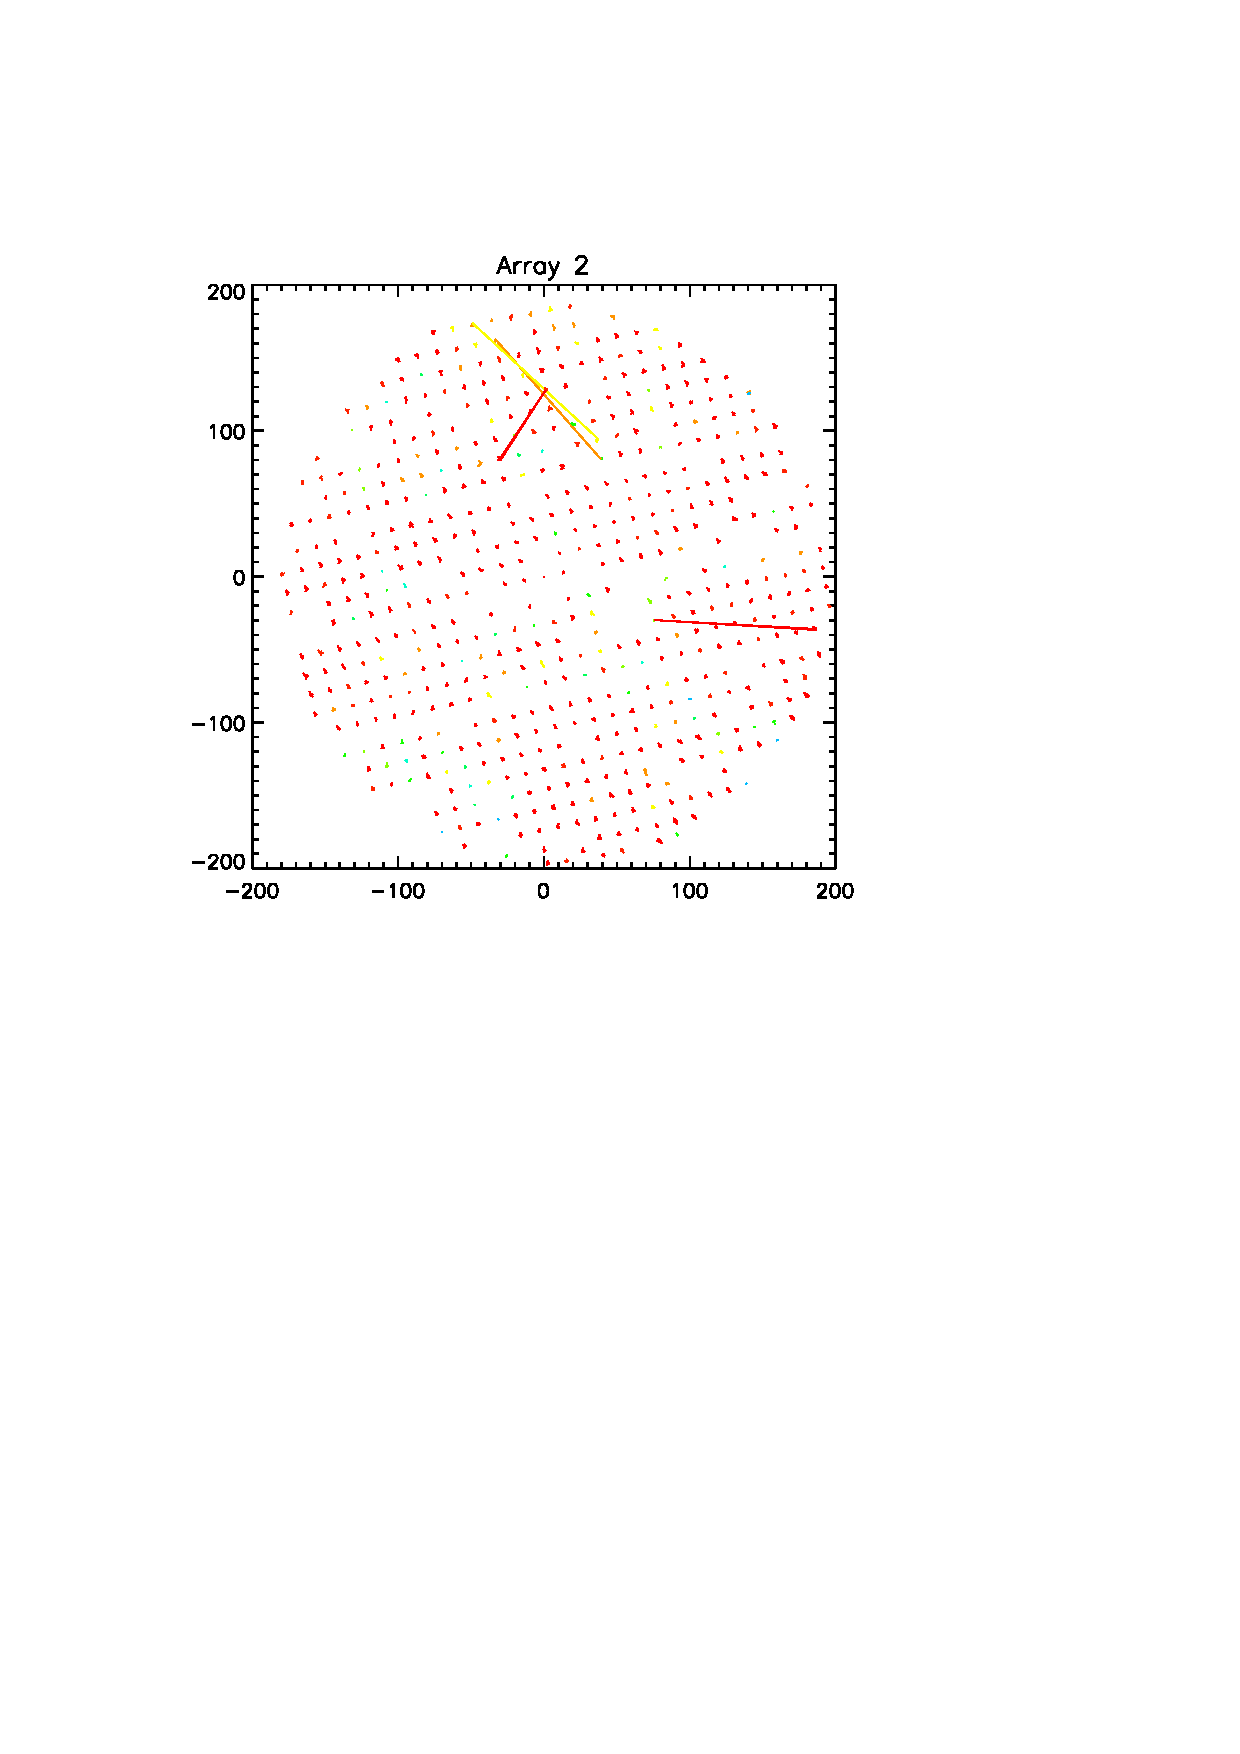
\includegraphics[trim=2cm 14cm 5cm 4cm, clip=true,width=0.45\linewidth]{Figures/A2_positions.pdf}
\caption[La sélection des KID]{Géométrie moyenne des matrices A1, A3
  et A2. Chacune des figures montre la position des détecteurs
  dans le plan focal, en secondes d'arc, ainsi que leur lobe modélisé par une
  gaussienne elliptique. Elles incluent les détecteurs qui ont été sélectionnés
  dans au moins deux analyses de {\tt beammaps}, correspondant à 952,
  961, and 553 KID pour A1, A3 et A2, respectivement.
  Les couleurs indiquent le nombre de fois qu'un KID a été
  sélectionné, depuis le bleu pour les KID sélectionnés dans deux
  analyses, jusqu'au rouge pour les KID sélectionnés dans les dix
  analyses (en passant par bleu ciel (3/10),
  cyan (4/10), céladon (5/10), vert (6/10), vert-jaune (7/10), jaune (8/10), orange (9/10)) 
  Les cercles en lignes interrompues correspondent à des disques de
  diamètres 5,5\,arcmin and 6,5\,arcmin.}
\label{fig:avg_fov_color}
\end{center}
\end{figure}

La sélection finale est obtenue par comptage du nombre
de fois qu'un KID a été sélectionné dans un ensemble de {\tt
  beammaps}. Le résultat de ce comptage est symbolisé par les couleurs
à la figure~\ref{fig:avg_fov_color} : depuis le bleu, indiquant les KID
sélectionnés dans deux analyses, jusqu'au rouge, pour les KID
sélectionnés dans les dix analyses. Nous définissons les KID
"valides'', c'est-à-dire à utiliser pour l'exploitation scientifique,
comme ceux qui ont été sélectionnés dans au moins 20\% des analyses de
{\tt beammaps} (2/10). Nous trouvons une fraction de KID valides de
84\% à 1\,mm et de 90\% à 2\,mm. Par ailleurs, l'ensemble du champ de
vue de 6,5' de diamètre, repéré par le cercle externe à la
figure~\ref{fig:avg_fov_color}, est bien couvert par les détecteurs
pour les trois matrices. 




%----------------------------------------------------------------------------------------
%
%   Lobe
%
%----------------------------------------------------------------------------------------
\section{Le lobe}
\label{se:beam}

Le lobe de NIKA2 résulte de l'illumination par les détecteurs de l'ensemble
du système optique jusqu'au miroir primaire du télescope. Le lobe
total présente une structure complexe, incluant un lobe principal, des
lobes d'erreurs provenant de la déformation d'ensemble du miroir
primaire, et des lobes lointains résultant de la diffraction par
différentes structures composant le système optique. Nous en donnons
une description qualitative à la Sect.~\ref{se:fullbeam}, puis nous
estimons les paramètres du lobe déterminant les performances de NIKA2
à la Sect.~\ref{se:mainbeam} : la largeur à mi-hauteur (FWHM) du lobe
principal, définissant la résolution angulaire de l'instrument, et
l'efficacité du lobe principal, influant sa sensibilité. Finalement,
nous mesurons les variations temporelles du lobe principal à la
Sect.~\ref{se:fwhm_variations}.


\subsection{La structure du lobe total}
\label{se:fullbeam}

La structure du lobe total est mise en évidence en combinant plusieurs
{\tt beammaps} vers des sources compactes brillantes.
%%
\begin{figure}[!thbp]
\begin{center}
  \includegraphics[trim=0.5cm 0.5cm 1cm 0cm, clip=true, width=\linewidth]{Figures/NIKA2/Lobe_map_Combo_v2_dB_2.pdf}
\caption[Noticeable features of NIKA2 beam pattern.]{Cartographie du
  lobe de la combinaison des matrices à 1\,mm (A1$\&$3) and de la
  matrice à 2\,mm (A2) en décibels. Ces cartes sont construites à
  partir d'une combinaison de {\tt beammaps} vers des sources
  ponctuelles brillantes; elles sont en coordonnées horizontales et
  couvrent une zone du ciel de $10'$ de coté. En plus du lobe pricipal
  et des premiers lobes d'erreur et lobes lointains au centre, elles
  présentent plusieurs structures notables (comme l'anneau de
  diffraction à 1\,mm, les figures de diffraction par les pieds
  supportants le miroir secondaire à 2\,mm) qui sont commentées dans le
  texte.}
\label{fig:features}
\end{center}
\end{figure}
%%
\`A la figure~\ref{fig:features}, nous présentons une cartographie du lobe
total incluant quatre {\tt beammaps} vers Uranus, Neptune et le quasar
3C84. Des cartes sont produites à partir de chaque {\tt beammap} en
utilisant le \emph{pipeline} d'analyse décrit à la
Sect.~\ref{se:pipeline}, puis elles sont normalisées et recentrées avant d'être
co-additionnées. Les cartes finales mettent au jour la structure du
lobe sur quelques minutes d'arc, les plus grandes échelles angulaires
étant filtrées par la méthode d'analyse. Elles révèlent une structure
complexe incluant 1) le lobe principal (point central) et les premiers
lobe d'erreur et lobes lointains du télescope, visibles au centre à un
niveau jusqu'à -20 décibel, 2) un anneau de rayon environ 110'',
visible à un niveau bien plus faible (-30\,dB) à 1\,mm, et qui
tirerait son origine de la diffraction par les jointures des panneaux
composant le miroir primaire~\citep{Greve2010}, 3) deux diagonales,
visibles également vers -30\,dB sur la carte à 2\,mm, créées par la
diffraction par la structure (quadrupode) supportant le miroir
secondaire, 4) d'autres petites structures à des niveaux situés en
deçà de -20\,dB, d'origine incertaines, ayant très peu d'impact sur
les observations.


Une autre manière de caractériser le lobe total, permettant de mesurer
les contributions relatives des principales structures le composant,
consiste à mesurer son profil radial. Celui-ci est obtenu en moyennant
les pixels de la carte du lobe dans des anneaux concentriques autour
du lobe principal. \`A la figure~\ref{fig:beam_prof}, nous traçons les
profils du lobe mesurés à partir de 18 {\tt beammaps}. Ce jeu de {\tt
  beammaps} nous permet de tester la stabilité du profil du lobe sous
différentes conditions d'observation (densité de flux de la source,
conditions atmosphériques, élévation, optimisation du focus). La
dispersion des profils par rapport au profil médian est de $5\%$ à
1\,mm et $2\%$ à 2\,mm, indiquant une bonne stabilité. Par ailleurs,
le profil du lobe est bien mesuré jusqu'à un rayon d'environ
180''.

\begin{figure}[!thbp]
  \centering
   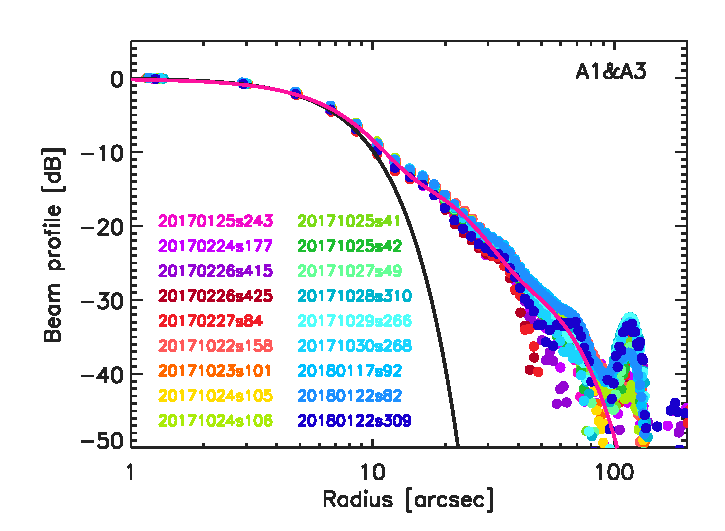
\includegraphics[clip, width=0.45\linewidth]{Figures/NIKA2/plot_profiles_dB_1mm.pdf}
   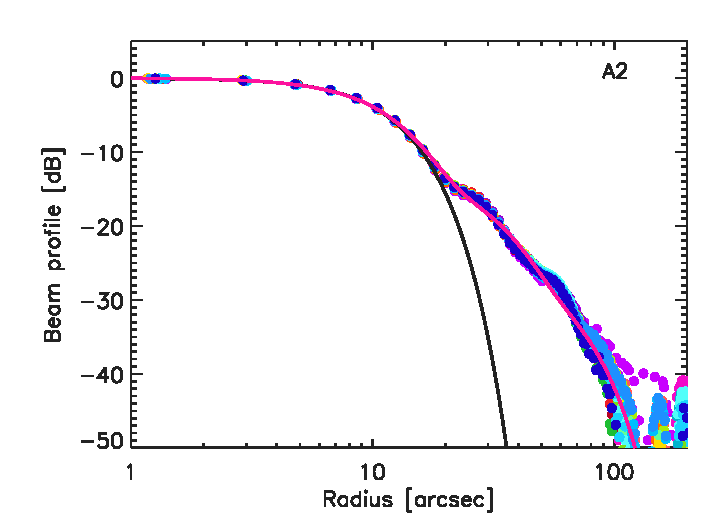
\includegraphics[clip, width=0.45\linewidth]{Figures/NIKA2/plot_profiles_dB_a2.pdf}
   \caption[Stability of the beam profile]{Profiles radiaux des lobes
     à 1\,mm (à gauche) et 2\,mm (à droite) tracés en décibels en
     fonction de la distance radiale au centre du lobe. Les points
     correspondent à la mesure du profile du lobe pour une série de 18
     {\tt beammaps} vers des sources compactes brillantes observés
     lors des campagnes de référence. Ils sont repérés par
     l'identifiant du scan de {\tt beammaps}. La courbe rose montre le
     modèle 3G calculé à partir de la médiane des meilleurs ajustement
     sur chacun des profiles. La courbe noire représente le meilleur
     ajustement d'une gaussienne au lobe principal.}
  \label{fig:beam_prof}
\end{figure}

Pour estimer les contributions relatives des premiers lobes
d'erreur et lobes lointains, nous modélisons le profil par une
combinaison linéaire de trois gaussiennes (3G). Un profil 3G est
ajusté à chacun des 18 profils mesurés et la médiane des meilleurs
ajustements est tracée à la figure~\ref{fig:beam_prof}. Nous mesurons
la contribution du premier lobe d'erreur par rapport au lobe total à
-11\,dB à 1\,mm et à -13\,dB à 2\,mm. Le lobe principal, modélisé par
une gaussienne, est tracé en noir à la figure~\ref{fig:beam_prof}. 


\subsection{Le lobe principal}
\label{se:mainbeam}

\subsubsection{La FWHM}

Le lobe principal est bien modélisé par une gaussienne. L'ajustement
de cette gaussienne aux cartes ou aux profils du lobe total doit
prendre en compte la contribution des lobes d'erreur et lobes
lointains. Pour cela, trois méthodes ont été développées. La première
repose sur l'ajustement d'un profil 3G (Sect.~\ref{se:fullbeam}) : la
première gaussienne correspondant au lobe principal tandis que les
deux autres capturent les autres contributions au lobe total. Les deux
autres méthodes consistent à ajuster une unique gaussienne au lobe
total, en masquant les distances radiales pour lesquelles la
contribution des lobes d'erreur et lointains est significative. Ces
méthodes sont détaillées dans~\citet{Perotto2019}. Testées sur
plusieurs jeux de données, variant de part la stratégie de scans ({\tt
OTF}-scans ou {\tt beammaps}), les sources observées et les campagnes
d'observation, ces méthodes donnent des résultats cohérents et
compatibles, indiquant la robustesse de la mesure de la FWHM du lobe
principal.


Nous testons en particulier, la stabilité des FWHM mesurées pour des
conditions atmosphériques variables. Pour cela, nous avons constitué
un jeu de données comprenant environ 150 scans OTF vers des sources
compactes dont le flux excède 1\,Jy dans les deux bandes de fréquence,
sélectionnés en appliquant les critères définis à la
Sect.~\ref{se:scan_selection} aux trois campagnes d'observation de
référence. \`A la figure~\ref{fig:fwhm_map_atmtrans}, les mesures de
la FWHM effectuées à partir de ce jeu de données sont tracées en
fonction de la transmission atmosphérique, modélisée par
$\exp{(-\taunu\,x)}$. Le code de couleur indique la campagne
d'observation lors de laquelle a été acquis le scan. Nous concluons
que les mesures de la FWHM sont en accord pour les trois campagnes de
référence, et n'observons par d'effet systématique significatif
dépendant de la transmission atmosphérique.
%
\begin{figure}[!thbp]
\begin{center}
  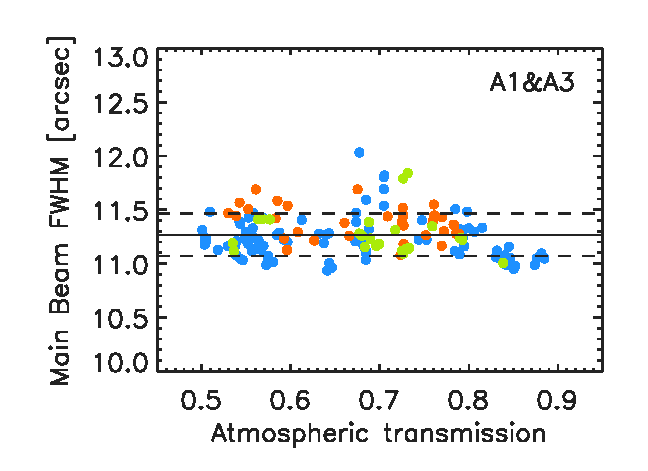
\includegraphics[clip, width=0.4\textwidth]{Figures/NIKA2/plot_FWHM_vs_atmtrans_mb_radius_binning2_1mm.pdf}
  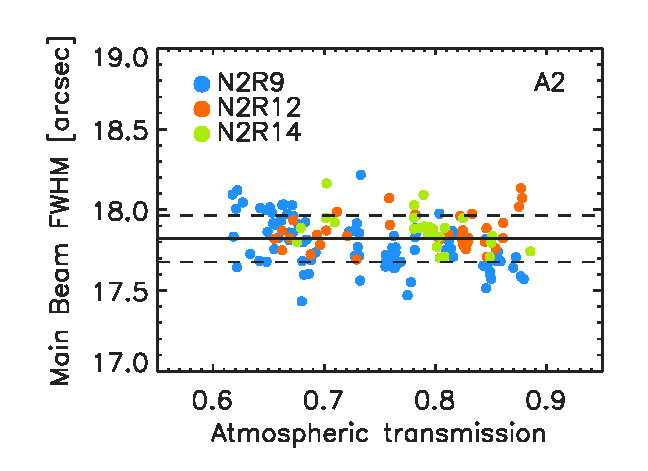
\includegraphics[clip, width=0.4\textwidth]{Figures/NIKA2/plot_FWHM_vs_atmtrans_mb_radius_binning2_a2.pdf}
  \caption[Main Beam FWHM]{Estimations de la largeur à mi-hauteur
    (FWHM) du lobe principal modélisé par une gaussienne, pour la bande à 1\,mm
    (à gauche) et à 2\,mm (à droite). Les FWHM sont mesurées à partir
    d'une série d'observations de sources compactes de flux $>1\,$Jy
    effectuées lors des trois campagnes de référence (N2R9, N2R12,
    N2R14); elles sont tracées en fonction de la transmission de
    l'atmosphère au moment de l'observation, qui dépend de l'opacité
    de l'atmosphère le long de la ligne de visée, $\taunu \, x$,
    suivant $\exp{(-\taunu \, x)}$. }
\label{fig:fwhm_map_atmtrans}
\end{center}
\end{figure}
%
En combinant les résultats des tests effectués avec différentes
méthodes d'estimation et différent jeux de données, nous obtenons une
mesure robuste de la FWHM et de son incertitude. Le lobe principal est
caractérisé par une FWHM de $11,1'' \pm 0,2''$ à 260\,GHz et de
$17,6'' \pm 0,1''$ à 150\,GHz. Ces performances sont meilleures que
les spécifications définies dans MoU. 


\subsubsection{L'efficacité}

L'efficacité du lobe principal est définie comme l'angle solide
sous-tendu par le lobe principal rapporté à l'angle solide du lobe
total. L'angle solide du lobe principal (\emph{main beam}) se calcule
directement à partir de la FWHM suivant $\Omega_{\rm{mb}} = 2\pi\,
(8\ln{2} \, \rm{FWHM}^2)$. L'angle solide du lobe
total jusqu'à une distance radiale maximale $r_{\rm{max}}$ est évalué suivant
\begin{equation}
  \Omega_{r_{\rm{max}}}(\nu) = \int_0^{r_{max}} B_{\nu}(r) \,  2 \pi r dr
  \label{eq:omega_rmax}
\end{equation}
à partir du profil normalisé du lobe total $B_{\nu}(r)$ pour la
matrice $\nu$. Nous le mesurons dans les cartes produites à partir de
{\tt beammaps} vers une source ponctuelle jusqu'à
$r_{\rm{max}}=180''$. Cette limite est imposée à la fois par la
stratégie de balayage, qui détermine l'homogénéité et le niveau de
bruit dans les cartes, et par le filtrage des grandes échelles
angulaires induit par le \emph{pipeline} d'analyse
(Sect.~\ref{se:pipeline}). \`A partir des mesures du profil du lobe
total et de la FWHM du lobe principal, nous estimons une efficacité de
$55 \pm 3\%$ à 260\,GHz et de $77 \pm 2\%$ à 150\,GHz.

Des études dédiées au lobe du télescope de 30-m ont qu'une
fraction significative du lobe se situe à des distances radiales au-delà
de 180''~\citep{Greve1998, Kramer2013}. Dans \citet{Kramer2013}, le
profil du lobe total a été mesuré à partir d'observations des limbes
de la Lune et modélisé par un lobe principal et trois lobes d'erreurs
gaussiens. Cette étude évalue également les contributions aux grandes échelles
angulaires à l'efficacité, issues du \emph{spillover}
(lumière parasite issue de l'atmosphère et du sol) et de Ruze (effet
des écarts de la surface du miroir primaire à la forme parabolique), à
partir d'observations de type {\tt skydip} effectuées avec le
\emph{Eight Mixer Receiver} (EMIR, \citet{Carter2012}),
l'instrument hétérodyne installé au télescope de 30-m. En nous fondant
sur ces résultats, nous évaluons l'angle solide du lobe total comme
\begin{equation}
  \Omega_{\rm{tot}} = \Omega_{180} + \Omega_{>180}^{\rm{mb+eb}} +
  \Omega^{\rm{frss}},
  \label{eq:omega_tot}
\end{equation}
où $\Omega_{180}$ est la mesure de l'angle solide du lobe total
jusqu'à 180'' estimée en utilisant Eq.~\ref{eq:omega_rmax},
$\Omega_{>180}^{\rm{mb+eb}}$ est la contribution des distances
radiales $>180''$ à l'angle solide issue du lobe principal (mb) et des
lobes d'erreur (eb) modélisés suivant~\citet{Kramer2013}, et
$\Omega^{\rm{frss}}$ représente les contributions du \emph{spillover}
et de la dispersion de Ruze. Ces différents termes sont évalués
dans~\citet{Perotto2019}. Chacun représente entre 7 et 15\% de l'angle
solide total. Cette caractérisation de l'angle solide total
est nécessaire à l'étude des sources diffuses ou aux mesures de flux
par photométrie d'ouverture, comme discuté plus loin, à la
Sect.~\ref{se:calibration}.


\subsection{Variation journalière}
\label{se:fwhm_variations}

\`A partir de tests de stabilité du lobe principal, nous
avons mis au jour une variation journalière de la FWHM. Cette
variation consiste en une lente augmentation de la FWHM, débutant
après le lever du Soleil et devenant significative dans l'après-midi,
puis un retour vers la valeur nominale (nocturne) après le coucher du
Soleil. Cet effet est présenté à la
figure~\ref{fig:beam_monitoring_otf} rassemblant les mesures de la
FWHM effectuées à partir d'une série de scans OTF vers des sources
compactes brillantes, et tracées en fonction de l'heure
d'observation. Une même évolution globale de la FWHM durant la journée
est observée lors des trois campagnes de référence. Cette variation
journalière est indépendante du flux de la source, puisqu'elle reste
la même aussi bien à partir des scans vers les planètes géantes Uranus
et Neptune que vers d'autres sources compactes moins brillantes. Par
ailleurs, d'importantes variations sont observées autour de la
tendance globale.
%
\begin{figure}[ht!]
  \begin{center}
    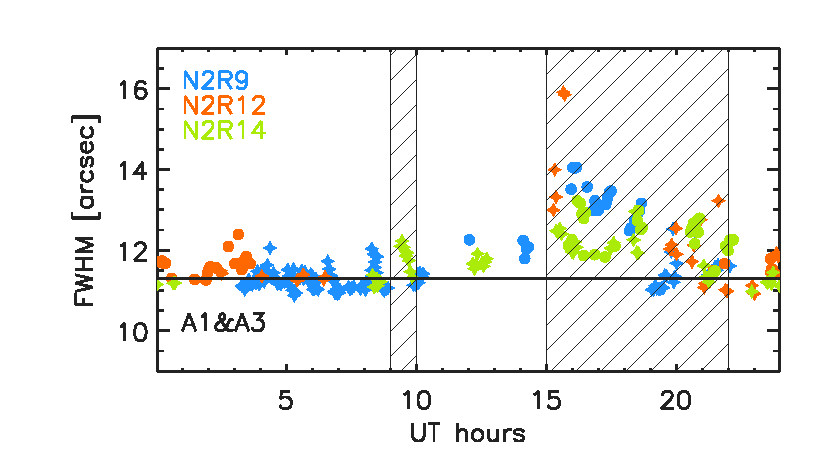
\includegraphics[clip=true, trim={0.9cm, 0.5cm, 0.5cm, 0.5cm}, width=0.4725\textwidth]{Figures/NIKA2/Beam_monitoring_with_otfs_vs_ut_1mm.pdf}
    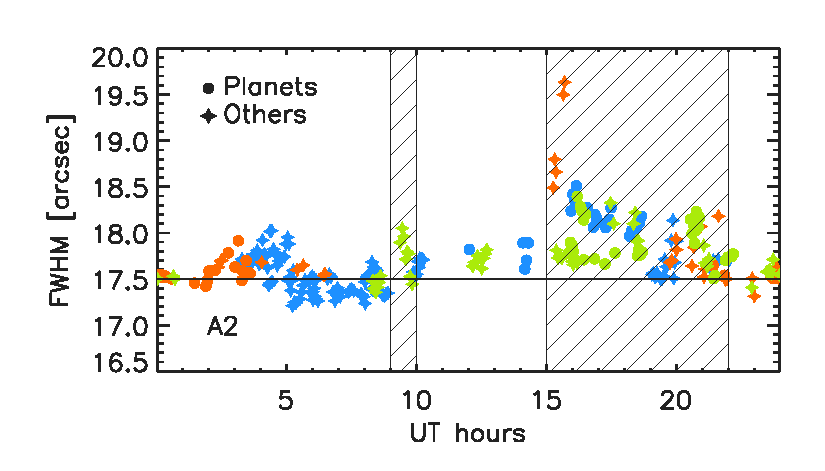
\includegraphics[clip=true, trim={0.5cm, 0.5cm, 0.5cm, 0.5cm}, width=0.4875\textwidth]{Figures/NIKA2/Beam_monitoring_with_otfs_vs_ut_a2.pdf}
    \caption[Beam size monitoring using OTF scans]{Suivi des
      variations journalières de la taille apparente du lobe. La
      largeur à mi-hauteur (FWHM) du lobe, modélisé par une gaussienne
      elliptique, est tracée pour la bande à 1\,mm (à gauche) et à
      2\,mm (à droite) en fonction du moment d'observation exprimé en
      heures UTC. Les mesures sont effectuées à partir de scans vers
      les planètes géantes (points) et vers d'autres sources
      compactes de flux $>1\,\rm{Jy}$ (étoiles) observés durant les
      trois campagnes de référence. Les zones hachurées correspondent
      aux périodes d'observation exclues par la sélection
      \emph{baseline} des scans, décrite à la Sect.~\ref{se:scan_selection}.} 
\label{fig:beam_monitoring_otf}
  \end{center}
\end{figure}

Cette variation journalière résulte probablement de la combinaison de
deux phénomènes liés à la température extérieure. Tout d'abord, le
chauffage inhomogène du miroir primaire du télescope, par exemple sous
l'effet de l'illumination partielle par la lumière solaire, entraîne
des déformations d'ensemble, qui à leur tour, le défocalisent
légèrement. L'impact de cet effet est réduit grâce au système de
thermalisation qui équipe le miroir primaire (voir
Sect.~\ref{se:observations}), mais dans les cas de forts gradients de
température d'un bout à l'autre des 30\,m de diamètre, un effet
résiduel peut apparaître. Ces variations journalières sont connues au
télescope de 30-m : elles affectent également les observations de
l'instrument EMIR et avaient été mises en évidence avec
MAMBO-2~\citep{Kreysa1999}, l'instrument ayant précédé l'installation
de NIKA et NIKA2. Cependant, l'amplitude de l'effet est certainement
en augmentation depuis quelques années, avec la progressive
dégradation de la peinture blanche recouvrant le miroir primaire.

Le deuxième effet qui participe de la variation journalière du lobe,
est la réfraction anormale de l'atmosphère. Ce phénomène, qui a été
décrit pour le télescope de 30-m dans~\citet{Altenhoff1987}, consiste
en de petites variations sur des temps courts de l'indice de
réfraction de l'atmosphère. Il survient, par exemple, quand de petites
masses d'air chaudes et humides s'élèvent du sol et traversent le
faisceau du télescope. Le pointage du télescope varie alors légèrement
pendant quelques secondes, l'effet moyen de ces variations induisant
un élargissement du lobe. Avec NIKA2, il est possible de repérer les
observations affectées par la réfraction anormale en utilisant les
scans de pointage. Une petite carte est produite à partir de chacun
des quatre subscans d'un {\tt pointage} (voir
Sect.~\ref{se:pointing}). Les écarts entre les mesures de la
position du lobe sur chacune des cartes nous donne un indicateur de
la réfraction anormale. Ainsi, celle-ci est responsable de
l'élargissement apparent du lobe pour entre le tiers et la moitié des
observations affectées par la variation journalière.  


Pour en limiter l'impact sur les performances de l'instrument, nous
excluons les observations effectuées aux moments de la journée les
plus affectés par l'élargissement apparent du lobe. Ces périodes,
repérées par les zones hachurées sur la
figure~\ref{fig:beam_monitoring_otf}, correspondent au lever du Soleil
(de 9\,h à 10\,h UTC) et à l'après-midi jusqu'à quelques heures après
le coucher du Soleil (de 15\,h à 22\,h UTC). Ces coupures sont inclues
à la sélection des scans (voir Sect.~\ref{se:scan_selection}).




%----------------------------------------------------------------------------------------
%
%   Atmosphere
%
%----------------------------------------------------------------------------------------
\section{La correction atmosphérique}
\label{se:opacity}

L'atténuation du signal par l'atmosphère est la limite indépassable
des expériences millimétriques au sol. Celle-ci résulte de multiples
phénomènes physiques, dominés par l'absorption par la vapeur d'eau,
mais incluant aussi l'effet de molécules di-électriques telles
l'oxygène ou la présence de particules dispersives (gouttelettes,
glace)~\citep{Pardo2002, Pardo2001}. Même dans les fenêtres de
transparence de l'atmosphère, qui imposent leur bande passante aux
instruments (voir Sect.~\ref{se:bandpass}), le signal est fortement
atténué. La densité de
flux $\tilde{S}_\nu$ reçue au sol dans la bande passante $\nu$ est
reliée à la densité de flux au-dessus de l'atmosphère $S_\nu$ par
\begin{equation}
  \tilde{S}_\nu = S_\nu \, e^{-\taunu \, x},
\end{equation}
où $\taunu$ est l'opacité de l'atmosphère dans la bande passante $\nu$
et $x$, l'extension de la masse d'air traversée. Dans un modèle
d'atmosphère plan-parallèle, la masse d'air dépend de l'élévation
comme $x = 1/\sin{\elev}$. Une mesure précise de $\taunu$ est donc
critique pour l'estimation des densités de flux. Pour cela, nous avons
développé deux méthodes, qui sont brièvement décrites à la
Sect.~\ref{se:opacity_methods} et comparées à la
Sect.~\ref{se:opacity_tests}.


\subsection{Méthodes}
\label{se:opacity_methods}

Pour mesurer l'opacité atmosphérique à chaque scans, nous utilisons
deux méthodes. L'une, standard aux instruments équipant le télescope
de 30-m, consiste à exploiter les mesures effectuées par le tau-mètre
à demeure. L'autre est originale aux expériences NIKA et NIKA2 et
permet une mesure de l'opacité par les détecteurs-même de NIKA2.  

\subsubsection{Interpolation des mesures du tau-mètre résident}

Le télescope de 30-m est équipé d'un tau-mètre mesurant l'opacité
atmosphérique à 225\,GHz, $\tau_{225}$, au moyen de skydips à une
azimut fixe. Une mesure de $\tau_{225}$ est effectuée toutes les
quatre minutes, permettant un suivi des conditions atmosphériques. La
série temporelle des mesures de $\tau_{225}$ est mise à disposition
par les équipes d'analyse de l'IRAM, après traitement des données du
tau-mètre. Nous interpolons ces mesures à la fois aux temps auxquels
sont observés les scans de NIKA2, et aux bandes passantes. Les séries
temporelles de $\tau_{225}$ sont interpolées à chaque échantillon des
données de NIKA2 puis lissées par une moyenne glissante. Pour obtenir
une estimation de l'opacité atmosphérique dans les bandes passantes de
NIKA2 $\taunu$, nous avons observé un calibrateur dans une large
gamme d'élévations et de conditions atmosphériques. Nous ajustons un
modèle linéaire entre $\taunu$ et $\tau_{225}$ sous contrainte de
garder le flux du calibrateur quelque soit les conditions
d'observation. L'avantage de cette méthode est d'être indépendante à
la fois des modélisations de l'atmosphère et des mesures en
laboratoire des bandes passantes. 

\subsubsection{Mesures NIKA2 calibrées par les {\tt skydips}}

L'opacité atmosphérique peut être mesurée directement par les
détecteurs de NIKA2, après avoir calibrée la relation entre les
variations de la fréquence de résonance des KID et la température
effective de l'atmosphère. Cette méthode originale a été développée et
validée avec le prédécesseur NIKA~\citep{Catalano2014}. Son avantage
principal est de fournir une mesure pour chaque scan et dans les
bandes passantes de NIKA2, sans nécessité d'interpoler en temps ou en
fréquence. Par ailleurs, la mesure est réalisée à l'azimut du scan,
limitant la dispersion due aux variations spatiales de l'atmosphère.

En pratique, la fréquence de résonance $f_{\rm{reso}}$ pour le KID $k$
varie en fonction de la température effective du ciel vue par
NIKA2 $T_{\rm{sky}} = T_{\rm{atm}}[1-e^{-\taunu x}]$, pour une masse
d'air $x$ et une opacité atmosphérique $\taunu$ suivant 
%
\begin{equation}
f_{\rm{reso}}^k  = c_0^k - c_1^k T_{\rm{atm}}[1-e^{-\taunu x}],
\label{eq:skydip}
\end{equation}
%
où le coefficient $c_0^k$ correspond à la fréquence de résonance du
KID $k$ à opacité atmosphérique nulle et le coefficient $c_1^k$, sa
réponse en Hz/K à la température effective de l'atmosphère. La
température de l'atmosphère $T_{\rm{atm}}$ est fixée à
270\,K. Ce choix a peu d'impact sur l'estimation finale de $\taunu$
comme discuté dans~\citet{Perotto2019}. Une fois calibrée la relation
$f_{\rm{reso}}$-$\taunu$, c'est-à-dire lorsque les coefficients $c_0$ et
$c_1$ de chaque KID ont été estimés, il est possible de mesurer
$\taunu$ dans les données brutes de NIKA2 pour chaque scan, en
inversant Eq.~\ref{eq:skydip}.

Les coefficients $c_0$ et $c_1$ de chaque KID sont estimés à partir de
scans de {\tt skydip} (décrits à la Sect.~\ref{se:skydip}) nous
fournissant onze mesures à différentes masses d'air, correspondant à
des élévations entre 20 et $65\degree$. Aussi, nous
analysons conjointement une série de {\tt skydips} observés à des
opacités atmosphériques différentes afin de lever la dégénérescence
entre $c_1$ et $\taunu$. La procédure d'ajustement employée comporte
deux étapes. Tout d'abord, nous ajustons simultanément $c_0$, $c_1$ et
$\taunu$ pour tous les KID et tous les {\tt skydips}. Puis nous fixons
$\taunu$ à la meilleure estimée moyenne, pour ajuster uniquement les
coefficients $c_0$ et $c_1$ des KID.

Pour finir, les {\tt skydips} doivent être observés dans des
conditions atmosphériques compatibles avec l'hypothèse d'atmosphère
plan-parallèle qui sous-tend le modèle à l'Eq.~\ref{se:skydip}. Nous
procédons à une sélection des {\tt skydips} sur des critères de
qualité de l'ajustement de l'Eq.~\ref{se:skydip}. Ensuite, nous
répétons la procédure d'estimation des $c_0$, $c_1$ à partir des {\tt
  skydips} sélectionnés. Un exemple de l'ajustement des $c_0$, $c_1$
pour un KID est illustré à la figure~\ref{fig:skydipfitexample}. 
%
\begin{figure}[!htbp]
\begin{center}
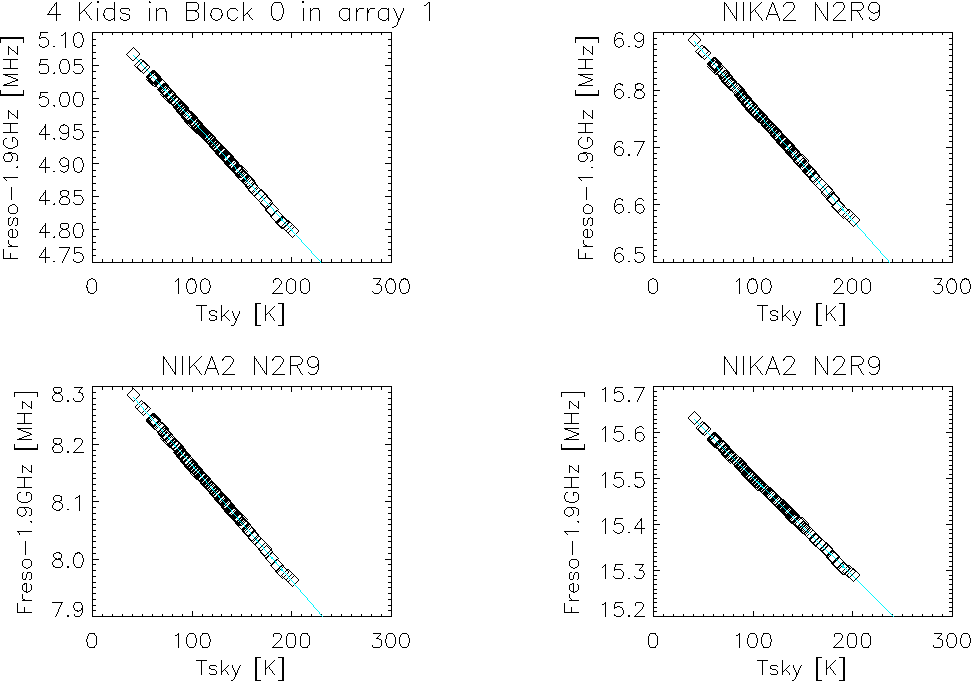
\includegraphics[trim={9cm 0cm 0cm 6.5cm}, clip=true, width=0.5\linewidth]{Figures/NIKA2/test_allskd4_N2R9v5_5-crop.pdf}
\caption[]{Exemple de la calibration de la réponse d'un KID à
  l'atmosphère. Chaque point (losange noir) représente la mesure de la
  fréquence de résonance du KID (par rapport à la valeur fixe de
  1,9\,GHz) pour l'un des paliers en élévation d'un scan de {\tt skydip}
  (Sect.~\ref{se:skydip}). Les points de mesures sont tracés en
  fonction de la température effective du ciel
  $T_{\rm{sky}} = T_{\rm{atm}}[1-e^{-\taunu\, x}]$ en Kelvin, où
  $\taunu$ est l'opacité atmosphérique telle qu'elle est ajustée. 
  La figure inclut les mesures réalisées à
  partir de 12 {\tt skydips} observés à des opacités atmosphériques
  $\taunu$ allant de 0,15 à 0,5 dans la bande à $1\,\rm{mm}$.
  La droite en bleu indique le meilleur ajustement du modèle donné à
  l'Eq.~\ref{eq:skydip}.}
\label{fig:skydipfitexample}
\end{center}
\end{figure}
%

\subsection{Tests des mesures d'opacité atmosphérique}
\label{se:opacity_tests}

Nous effectuons plusieurs tests de cohérence de l'estimation de
l'opacité atmosphérique. Tout d'abord, nous comparons les mesures
d'opacité obtenues avec les deux méthodes considérées, l'interpolation
au moment du scan des mesures du tau-mètre, $\tau_{225}$, et la mesure
dans les données brutes après calibration sur les {\tt skydips},
$\tau_{skydip}$, et ce, pour des observations réalisées au cours des
trois campagnes de référence. Les résultats sont présentés dans le
panel a) de la figure~\ref{fig:skydip-to-taumeter-correl}. La
corrélation entre les deux jeux de mesures de l'opacité reste stable
pour les trois campagnes d'observation. Cette stabilité entre les
résultats de deux méthodes indépendantes est une indication de la
robustesse de nos estimations de $\taunu$. Par ailleurs, nous
calculons une corrélation théorique entre $\tau_{skydip}$ et
$\tau_{225}$ en utilisant le modèle d'atmosphère ATM décrit
dans~\citet{Pardo2001}, les bandes passantes de NIKA2 telles qu'elles
ont été mesurées en laboratoire (Sect.~\ref{se:bandpass}) et une
étroite gaussienne centrée à 225\,GHz. Ces prédictions sont
représentées par les droites en noir à la
figure~\ref{fig:skydip-to-taumeter-correl}. Elles constituent un bon
modèle des corrélations mesurées à 1\,mm, mais tendent à sous-estimer
$\tau_{skydip}$ à 2\,mm. Cette différence peut avoir plusieurs
origines (erreur systématique dans les mesures de bande passante,
effet de la raie d'oxygène, etc.) mais n'a pas d'impact sur les
mesures de flux, puisque la calibration n'utilise ni modèle ATM, ni
les mesures des bandes passantes. Néanmoins, il est utile d'en garder
une trace afin de réitérer le test une fois qu'auront été effectuées
les mesures des bandes passantes de NIKA2 prévues au télescope de
30-m.
%
\begin{figure}[!thbp]
  \begin{center}
    \begin{overpic}[clip=true, trim={0, -0.3cm, -0.3cm, 0}, width=0.3\textwidth]{Figures/NIKA2/Opacity_correl_skydip_vs_tau_a1.pdf}
      \put(0,70){\footnotesize a)}
    \end{overpic}
    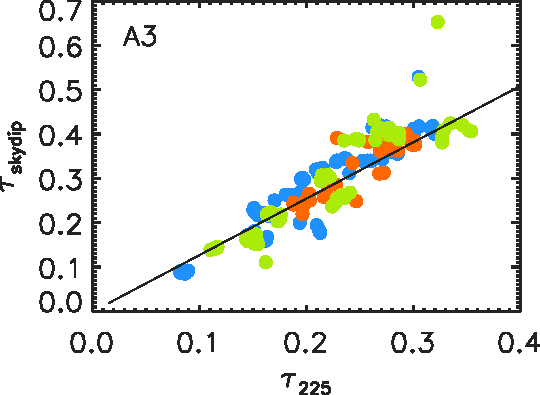
\includegraphics[clip=true, trim={0, -0.3cm, -0.3cm, 0}, width=0.3\textwidth]{Figures/NIKA2/Opacity_correl_skydip_vs_tau_a3.pdf}
    \begin{overpic}[clip=true, trim={-0.3cm, -0.3cm, 0, 0}, width=0.3\textwidth]{Figures/NIKA2/Opacity_skydip_to_taumeter_vs_elev_1mm.pdf}
      \put(0,70){\footnotesize b)}
    \end{overpic}
    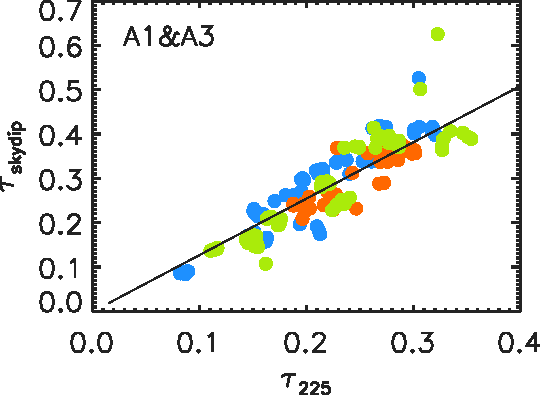
\includegraphics[clip=true, trim={0, -0.3cm, -0.3cm, 0}, width=0.3\textwidth]{Figures/NIKA2/Opacity_correl_skydip_vs_tau_1mm.pdf}
    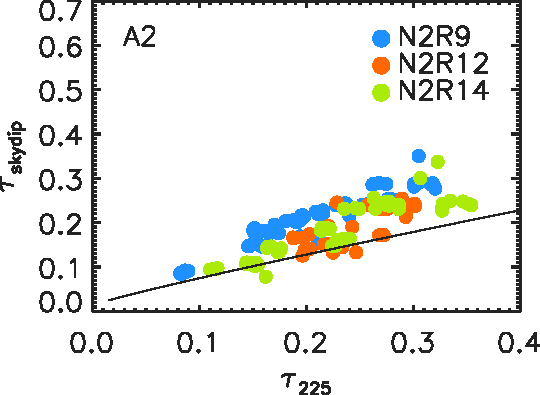
\includegraphics[clip=true, trim={0, -0.3cm, -0.3cm, 0}, width=0.3\textwidth]{Figures/NIKA2/Opacity_correl_skydip_vs_tau_a2.pdf}
    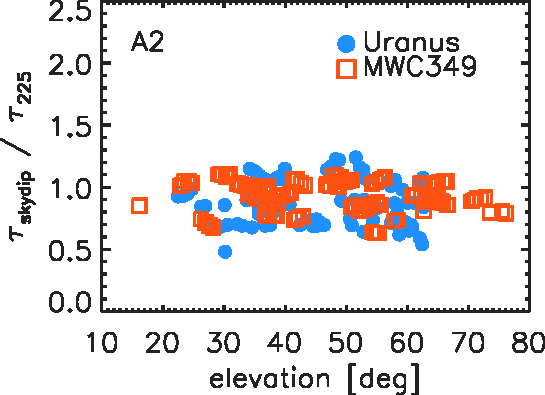
\includegraphics[clip=true, trim={-0.3cm, -0.3cm, 0, 0}, width=0.3\textwidth]{Figures/NIKA2/Opacity_skydip_to_taumeter_vs_elev_a2.pdf}
   \caption[]{Tests cohérence et de stabilité des estimations de
     l'opacité atmosphérique au zénith $\taunu$. a) Comparaison de
     $\taunu$ mesuré par NIKA2 après calibration avec les {\tt
       skydips}, noté $\tau_{\rm{skydip}}$, et de l'opacité mesuré par
     le tau-mètre à 225\,Ghz après interpolation au moment du scan et
     filtrage, $\tau_{225}$. La correlation $\tau_{\rm{skydip}}$ -
     $\tau_{225}$ est tracée pour une série de scans de calibrateurs
     observés lors des trois campagnes de référence. Un modèle de
     corrélation obtenu en intégrant un modèle ATM dans les bandes
     passantes de NIKA2 est aussi montré en noir à titre indicatif.  
     b) Le rapport $\tau_{\rm{skydip}}$ sur $\tau_{225}$ est tracé
     pour une large gamme d'élévation, à partir d'une série
     d'observations d'Uranus (points bleus) et du calibrateur
     secondaire MWC349 (carrés rouge).} 
\label{fig:skydip-to-taumeter-correl}
\end{center}
\end{figure}
%
Ensuite, nous testons une éventuelle dépendance de l'opacité
atmosphérique au zénith $\taunu$ avec la masse d'air $x$. Nous
calculons le rapport entre $\tau_{skydip}$ et $\tau_{225}$, définis
comme précédemment, et le traçons en fonction de l'élévation pour une
série de scans vers Uranus et vers un calibrateur secondaire
(MWC349). Les résultats sont présentés au panel b) de la
figure~\ref{fig:skydip-to-taumeter-correl}. Le rapport des mesures
d'opacité est stable pour une large gamme d'élévation allant de 15 à
$75\degree$. Cette stabilité est observée aussi bien pour les scans
d'Uranus, incluant plusieurs {\tt beammaps}, que pour les scans plus
courts vers MWC349. Ces tests indiquent la robustesse des estimations
d'opacité à l'élévation à laquelle sont effectuées les observations et
au type d'observation. 

Un ultime test de cohérence consistera à démontrer la stabilité des
flux mesurés après correction de l'atténuation de l'atmosphère à
partir de l'estimation de $\taunu$. Ce test sera présenté à la section
suivante (Sect.~\ref{se:calibration}). 



%----------------------------------------------------------------------------------------
%
%
%
%
%
%                 Calibration
%
%
%
%----------------------------------------------------------------------------------------
\section{Calibration absolue et relative}
\label{se:calibration}

Forts d'une reconstruction du plan focal, de la
caractérisation du lobe et de méthodes pour estimer l'atténuation de
l'atmosphère, nous avons tous les éléments en main pour réaliser la
calibration en flux. Pour cela, nous commençons par définir une
méthode de photométrie à la Sect.~\ref{se:systeme_photo}. Nous
effectuons une calibration relative entre les détecteurs, que nous
exploitons ensuite pour caractériser le plan focal à la
Sect.~\ref{se:gains}. Nous affinons l'estimation de l'opacité
atmosphérique à partir de tests photométriques à la
Sect.~\ref{se:corrected_skydip}. Nous résumons la méthode de
calibration \emph{baseline} à la Sect.~\ref{se:baseline_calibration}
et nous discutons une calibration alternative à la
Sect.~\ref{se:afternoon_calibration}.
        
\subsection{Système photométrique}
\label{se:systeme_photo}

\subsubsection{Le système de référence}

Notre photométrie procède de deux choix méthodologiques qui se fondent
sur des critères de simplicité et de robustesse. Tout d'abord, nous
mesurons les densités de flux à une fréquence fixe, $\nu_0$, choisie
arbitrairement, proche du centre de chaque bande passante. Ainsi,
$\nu_0 = 150$\,GHz dans la bande à 2\,mm et $\nu_0 = 260$\,GHz à
1\,mm. Modélisant la densité de flux d'un calibrateur primaire
$\rm{c}$ par $S_{\rm{c}} (\nu) = S_{\rm{c}} (\nu_0)\, f(\nu/\nu_0)$,
où $f(\nu/\nu_0)$ capture la dépendance spectrale, nous calibrons nos
densités de flux par rapport à $S_{\rm{c}} (\nu_0)$, sans intégration
dans les bandes passantes. Ces dernières n'étant utilisées que pour le
calcul des corrections de couleur, la propagation de leurs
incertitudes au flux mesuré est limitée pour la plupart des sources.
%
\begin{table}[!htbp]
\caption{Système photométrique de référence}
\label{tab:definitions}
\centering     
\begin{tabular}{lcc}
\hline\hline
      \noalign{\smallskip}
      & 1 mm & 2 mm \\
      \noalign{\smallskip}
      \hline
      \noalign{\smallskip}
      Fréquence de référence, $\nu_{0}$ & 260 GHz & 150 GHz \\
      FWHM de référence,  FWHM$_{0}$    & 12.5'' & 18.5'' \\
      \noalign{\smallskip}
      \hline
\end{tabular}
\end{table}
%

Le deuxième choix concerne la modélisation du lobe pour la mesure du
flux des sources ponctuelles. Comme présenté à la
Sect.~\ref{se:beam}, le lobe présente une structure complexe, avec
des lobes secondaires qui peuvent être asymétriques pour certaines
observations. L'ajustement de modèles complexes 2D (un template du
lobe) ou 1D (un profil) a été envisagé (et testé). Il s'accompagne
toutefois de difficultés, telles la dépendance aux conditions
d'observation (par exemple, la focalisation du télescope) et au
rapport signal-sur-bruit des données, qui détermine le niveau de
significance de la mesure des lobes secondaires. En revanche, nous
avons vérifié, sur des simulations et sur les données, qu'un modèle
simple du lobe assure une bonne stabilité des mesures de densité de
flux. Nous modélisons les cartes d'une source ponctuelle par une gaussienne
de référence dont la largeur à mi-hauteur (FWHM) est fixée à 
12,5'' à 1\,mm (260\,GHz) et de 18,5'' à 2\,mm (150\,GHz), soit
sensiblement plus grandes que la FWHM du lobe principal. La densité de
flux des sources correspond à l'amplitude de la gaussienne de
référence pour chacune des cartes. Les valeurs de référence FWHM$_0$ ont
été optimisées pour NIKA de façon à assurer la robustesse des mesures
des flux à l'effet des lobes secondaires. Nous avons vérifié cette
robustesse pour NIKA2 et nous avons aussi testé la stabilité des
mesures de flux pour des choix de FWHM$_0$ légèrement différents. Ces
deux choix, $\nu_0$ et FWHM$_0$, définissent notre système
photométrique et sont résumés dans la table~\ref{tab:definitions}.

\subsubsection{La calibration absolue}
Notre calibrateur primaire principal est la planète géante
Uranus. Neptune est parfois également utilisée dans les cas où Uranus
n'est pas observable dans des conditions optimales. Les densités de
flux attendues pour les deux planètes géantes sont calculées à partir
des modèles basées sur~\citet{Morenothesis}, tels qu'ils sont fournis par
l'ESA, et utilisés pour la calibration du satellite
\emph{Herschel}~\citep{Bendo2013}. La calibration absolue est réalisée
en ajustant l'amplitude $A_{\rm{c}}(\nu)$ d'une gaussienne de largeur
fixée à FWHM$_0$ dans les cartes produites pour chaque matrice $\nu$,
à partir d'une observation de l'un des calibrateurs primaires
$\rm{c}$. Les coefficients de calibration absolue pour les matrices
$\nu$ sont de la forme $S_{\rm{c}}(\nu_0) / A_{\rm{c}}(\nu)$. Les
cartes sont alors calibrées en Jy/beam. Par conséquent, les densités
de flux d'une source ponctuelle sont mesurées à partir des cartes dans
les bandes $\nu$ en 1) ajustant l'amplitude de la gaussienne de
référence dans chacune des cartes et 2) en appliquant les corrections
de couleur comme détaillé dans~\citet{Perotto2019}.

\subsubsection{Le flux des sources diffuses}

Pour l'études des sources diffuses, les cartes calibrées en Jy/beam
doivent être corrigées de l'angle solide du lobe total, dont une
estimation est donnée à la Sect.~\ref{se:mainbeam}. Dans
\citet{Perotto2019}, nous distinguons deux corrections. Tout d'abord,
les cartes sont exprimées en Jy/sr en normalisant par l'angle solide sous-tendu
par la gaussienne de référence, $\Omega_0 = 2\pi \, \sigma_0^2$, avec
$\sigma_0 = 1/(2\sqrt{2 \log{2}})\, \rm{FWHM}_0$. Puis, nous prenons
en compte la fraction de flux contenue dans le lobe total en
corrigeant par l'efficacité de la gaussienne de référence, définie par
$\rm{BE}_{0}$ $=$ $\Omega_{0}$ $/$ $\Omega_{\rm{tot}}$.
L'estimation de l'efficacité
de référence utilise l'évaluation des différentes contributions à
$\Omega_{\rm{tot}}$, comme décrit à la
Sect.~\ref{se:beam}. L'efficacité de référence et les facteurs
correctifs à appliquer en fonction de l'étendue de la source
considérée, sont fournis dans~\citet{Perotto2019}.


\subsection{Les gains des détecteurs}
\label{se:gains}

En pratique, les calibrations relative et absolue sont réalisées
conjointement par l'estimation des gains des détecteurs lors de
l'analyse d'une {\tt beammap} vers un calibrateur primaire. Comme
décrit à la Sect.~\ref{se:FOV_geometry}, dans une procédure de
reconstruction du plan focal, les données brutes en Hz sont projetées
pour construire des cartes individuelles par KID pour chaque
matrice. L'amplitude de la gaussienne de
référence $A_k(\nu)$ est ajustée sur la carte du KID $k$ pour la
matrice $\nu$. Les gains des KID sont définis par
\begin{equation}
  G_k(\nu) = \frac{S_{\rm{c}}(\nu_0)\, e^{-\taunu\,x}}{A_k(\nu)},
  \label{eq:kid_gain}
\end{equation}
et correspondent donc aux coefficients de calibration à opacité
atmosphérique nulle, exprimés en Jy/Hz/beam. L'application de ces
coefficients aux TOI de chaque KID consiste bien en une calibration
absolue et relative.


Cette calibration repose sur l'analyse d'un seul scan. Pour améliorer
la précision de la calibration absolue, nous estimons un coefficient
correctif à partir d'une série de scans d'Uranus acquis tout au long
de la campagne d'observation. Ce coefficient est la moyenne sur tous
les scans des rapports flux attendu sur flux mesuré dans chacun des
scans.

Si les gains des KID, définis à l'Eq.~\ref{eq:kid_gain}, sont calculés
à des fins de calibration, leur distribution dans le champ de vue offre
une caractérisation intéressante des matrices de détecteurs. En effet,
le gain de chaque détecteur réalise un échantillonnage dans le champ
de vue de la réponse de NIKA2 à une source ponctuelle située en champ lointain, le
\emph{main beam flat field}. Nous traçons les \emph{flat fields} des
trois matrices à la figure~\ref{fig:avg_mbff}. Ils ont été construits
en moyennant les gains relatifs mesurés sur une série de cinq
{\tt beammaps} observées lors des deux dernières campagnes
techniques. Les gains relatifs correspondent aux gains normalisés par
le gain moyen pour tous les détecteurs d'une matrice. 
 % 
\begin{figure}[!thbp] 
\begin{center}
  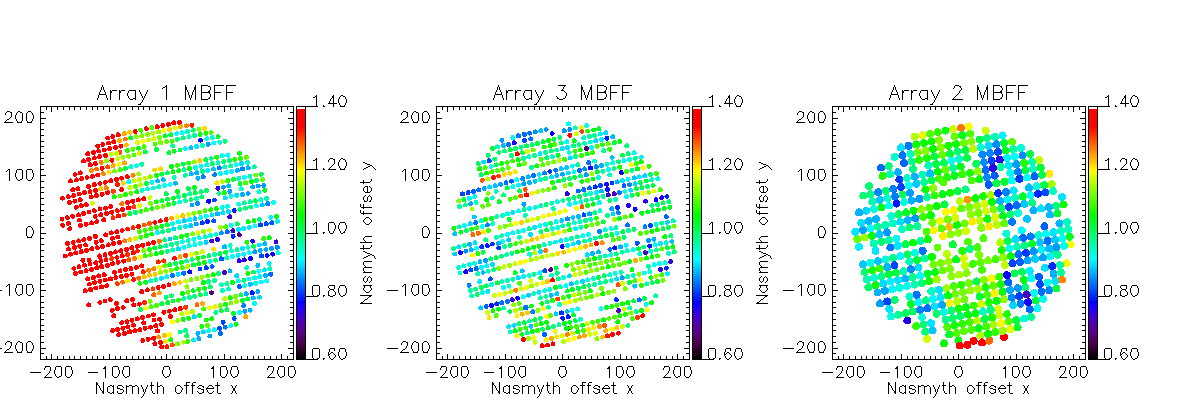
\includegraphics[width=0.95\textwidth]{Figures/NIKA2/Average_main_beam_flat_field_N2R9_10.png}
  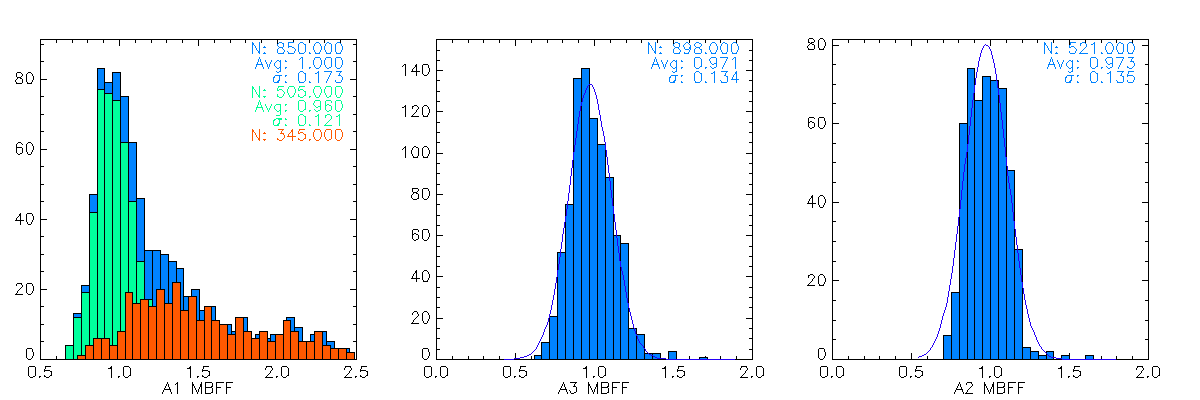
\includegraphics[width=0.8\textwidth]{Figures/NIKA2/Histo_average_main_beam_flat_field_N2R9_10.png}
  \caption[Average main beam flat fields]{\emph{Main Beam Flat
      Fields}. En haut, la distribution dans le champ de vue des gains
    relatifs des KIDs des matrices A1, A3 et A2. Les points indiquent
    la position de chaque détecteur par rapport au centre de la
    matrice, mesurée en secondes d'arc en coordonnées Nasmyth. Le code
    de couleur représente l'amplitude des gains relatifs, calculés
    suivant Eq.~\ref{eq:kid_gain} et normalisés par le gain moyen des
    détecteurs d'une matrice. En bas, les histogrammes des gains
    relatifs pour chaque matrice calculés en incluant soit tous les KIDs
    (en bleu), soit uniquement les KID du tiers gauche de la matrice
    A1 (rouge), soit uniquement les KID en dehors de ce tiers gauche
    (vert).}
 \label{fig:avg_mbff}
\end{center}
\end{figure}
%
Pour les matrices A3 et A2, les variations de gain sont d'amplitudes
faibles (rms d'environ $15\%$) et se répartissent dans le plan
focal suivant des structures pouvant être reliées à la connexion des
KID aux lignes de base de l'électronique de lecture. En revanche, pour
la matrice A1 nous observons une variation des gains de forte
amplitude, affectant environ un tiers des KIDs situés dans un
croissant à gauche de la matrice. Les distributions des gains relatifs
pour chaque matrice sont présentées en bas de la
figure~\ref{fig:avg_mbff}. La distribution pour A1 est
significativement élargie, et cet élargissement est dù aux gains des
détecteurs situés dans le tiers gauche du champ de vue. Les KIDs de
cette zone, qui pour un même signal (Jy) ont une réponse en Hz
moindre, semblent obscurcis. Par ailleurs, nous avons vérifié que cet
effet était également observé dans les \emph{flat fields} en champ
proche, en étudiant la réponse des KID à l'atmosphère, ce qui exclut
une origine liée au seul lobe principal.

Comme décrit à la Sect.~\ref{se:commissioning}, cet effet a été
observé pour la première fois après l'intervention sur l'instrument de
septembre 2016, au cours de laquelle la lame dichroïque, qui
présentait un défaut de planéité, avait été remplacée. De plus,
l'effet est bien reproduit par les simulations optiques incluant
un défaut de transmission de la lame dichroïque de l'une des composantes de
polarisation dans la bande à 1\,mm. Cette hypothèse a été directement
vérifiée en septembre 2018, par l'installation d'une troisième version
de la lame dichroïque, basée sur la technologie de la première version
(avant septembre 2016) et munie d'un support renforcé. Suite à cette
intervention, l'effet affectant le \emph{flat field} de A1 a bien
disparu, mais les défauts qui avaient motivés le remplacement de la
première génération de dichroïque sont réapparus. La lame dichroïque
de deuxième génération a été ré-installée pour revenir à la
configuration instrumentale post-septembre 2016. Ce défaut
de transmission de la composante de polarisation illuminant A1 a des
répercutions sur la sensibilité de cette matrice, comme discuté plus
avant à la Sect.~\ref{se:sensibilite}.      


\subsection{Tests photométriques de la correction de l'atmosphère}
\label{se:corrected_skydip}

Nous validons la calibration par des tests photométriques sur des
calibrateurs secondaires. Plusieurs sources de calibration sont
régulièrement suivies avec NIKA2, incluant des étoiles brillantes
(comme CRL2688), des nébuleuses planétaires faiblement résolues
(telles NGC7027). Parmi ces calibrateurs, le système d'étoiles binaire
MWC349~\citep{Tafoya2004} bénéficie de la prédiction la plus fiable du
flux attendu aux fréquences de NIKA2. En effet, pour cette source,
nous disposons d'observations effectuées à l'interféromètre du Plateau
de Bure (PdBI) et au \emph{Very Large Array} (VLA), permettant une
mesure précise de sa SED. Par ailleurs, l'incertitude liée à la
variabilité des calibrateurs secondaires est minimale pour MWC349,
car nous bénéficions d'un suivi régulier de cette source avec NOEMA,
pour lequel elle est un calibrateur. Cet exemple de synergie entre les
deux observatoires de l'IRAM a vocation à se développer. Pour finir,
MWC349 est une source ponctuelle pour le télescope de 30-m.

\`A partir de séries de scans OTF de $8' \times 5'$ vers MWC349
observés lors des trois campagnes de référence, nous testons la
stabilité des densités de flux mesurées aux conditions
atmosphériques. En particulier, nous testons les deux méthodes de
correction de l'opacité de l'atmosphère présentées à la
Sect.~\ref{se:opacity}. La figure~\ref{fig:mwc349_obstau_others}
montre le rapport flux mesuré sur flux attendu pour MWC349 en fonction
de la transmission atmosphérique sur la ligne de visée,
$\exp{(-\taunu \, x)}$. Cette figure inclut 72 scans sélectionnés sur
les critères \emph{baseline} (Sect.~\ref{se:scan_selection}). Dans les
panels du hauts, étiquetés \emph{taumeter}, la correction de
l'atténuation de l'atmosphère utilise les estimées de $\taunu$ issues
des mesures du tau-mètre à 225\,GHz
(Sect.~\ref{se:opacity_methods}). Dans les panels centraux, notés
\emph{skydip}, $\taunu$ est estimé via la calibration sur
les {\tt skydips} de NIKA2 (Sect.~\ref{se:opacity_methods}).  
%
\begin{figure}[!thbp]
  \begin{center}
    \begin{overpic}[clip=true, trim={0.9cm, 0.2cm, 0, 0.6cm},width=0.505\linewidth]{Figures/NIKA2/plot_flux_density_ratio_MWC349_obstau_tau225_narrow_1mm.pdf}
      \put(20,60){\footnotesize {\tt Taumeter}}
    \end{overpic}
    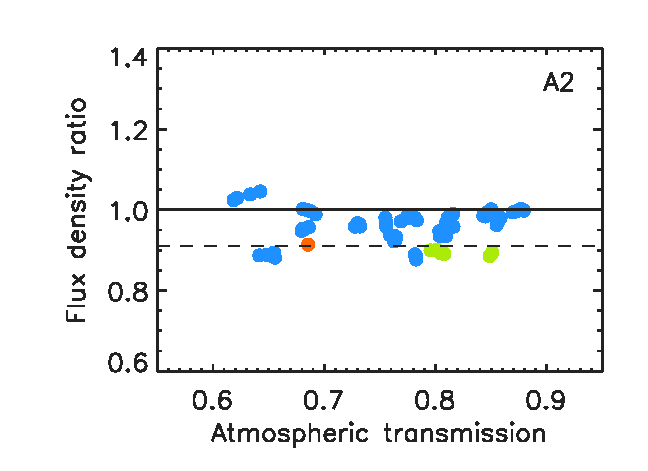
\includegraphics[clip=true, trim={1.8cm, 0.2cm, 0.5cm, 0.7cm},width=0.434\linewidth]{Figures/NIKA2/plot_flux_density_ratio_MWC349_obstau_tau225_narrow_a2.pdf}
    \begin{overpic}[clip=true, trim={0.9cm, 0.2cm, 0, 0.6cm},width=0.505\linewidth]{Figures/NIKA2/plot_flux_density_ratio_MWC349_obstau_skydip_narrow_1mm.pdf}
      \put(20,60){\footnotesize {\tt Skydip}}
    \end{overpic}
    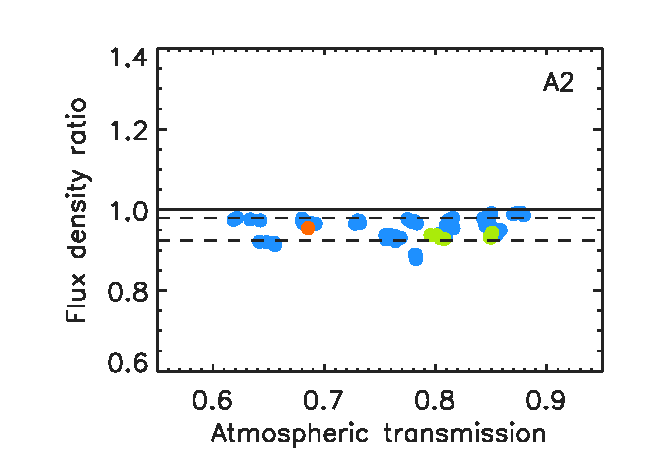
\includegraphics[clip=true, trim={1.8cm, 0.2cm, 0.5cm, 0.7cm},width=0.434\linewidth]{Figures/NIKA2/plot_flux_density_ratio_MWC349_obstau_skydip_narrow_a2.pdf}
    \vspace{-0.3cm}
    \begin{overpic}[clip=true, trim={0.9cm, 0.2cm, 0, 0.6cm},width=0.505\linewidth]{Figures/NIKA2/plot_flux_density_ratio_MWC349_obstau_corrected_skydip_narrow_1mm.pdf}
      \put(20,60){\footnotesize {\tt Baseline}}
    \end{overpic}
    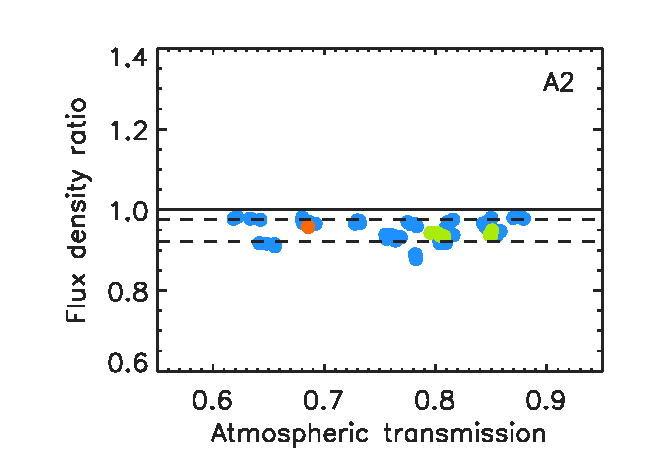
\includegraphics[clip=true, trim={1.8cm, 0.2cm, 0.5cm, 0.7cm},width=0.434\linewidth]{Figures/NIKA2/plot_flux_density_ratio_MWC349_obstau_corrected_skydip_narrow_a2.pdf}
    \caption[Calibration bias comparison]{Tests photométriques sur le
      calibrateur secondaire MWC349. Le rapport entre les densités de
      flux mesurées et attendues est tracé en fonction de la
      transmission de l'atmosphère, estimée par $\exp{(-\taunu x)}$,
      dans la bande à 1\,mm (à gauche) et à 2\,mm (à droite),   
      pour trois méthodes de calibration : en haut, label
      \emph{Taumeter}, $\taunu$ est estimé à partir des mesures du
      tau-mètre; au milieu, label \emph{Skydip}, l'estimation de
      $\taunu$ repose sur la calibration avec les \emph{skydips}; en
      bas, label \emph{baseline}, la méthode \emph{baseline} est
      utilisée. Les lignes pointillées correspondent à la rms des
      rapports de densité de flux.}
    \label{fig:mwc349_obstau_others}
  \end{center}
\end{figure}
%
Pour les deux méthodes, les flux mesurés sont en accord avec la
prédiction pour les trois campagnes d'observation et aux deux
fréquences. Le manque de flux de $5\%$ observé à 2\,mm reste
non-significatif, étant donné la précision de la prédiction du
flux. Pour \emph{taumeter}, les rapports de flux mesurés sont stables
dans toute la gamme de transmission atmosphérique testées, mais
présentent une plus grande dispersion que les rapports de flux
\emph{skydip}. Ce surcroit de dispersion est attendu étant donné que
l'opacité est estimée à l'azimut fixe du tau-mètre et non à l'azimut
du scan. Avec la méthode \emph{skydip}, nous observons un effet
systématique affectant les rapports de flux à 1\,mm, avec une
amplitude d'environ $15\%$ entre les
plus basses et les plus hautes transmissions atmosphériques. Cet effet
a motivé le recours à une correction des mesures d'opacité
\emph{skydip}.


\subsection{La méthode de calibration de référence}
\label{se:baseline_calibration}

Pour traiter l'atténuation des flux par l'atmosphère, la
calibration de référence, appelée \emph{baseline}, utilise une version
corrigée des opacités estimées avec la méthode de la calibration sur
les {\tt skydips} de NIKA2, que l'on notera
$\tau_{\rm{skydip}}$. Cette correction des $\tau_{\rm{skydip}}$
consiste en un facteur multiplicatif $a_\nu$ pour chaque matrice
$\nu$, qui est estimé à partir des densités de flux mesurées,
\begin{equation}
  S_\nu = \tilde{S}_\nu \,\,  e^{a_\nu \tau_{\rm{skydip}} x},
\end{equation}
sous une contrainte de stabilité dans la gamme de transmission
atmosphérique testée. Les facteurs $a_\nu$ modélisent la dégénérescence
entre $\taunu$ et $c_1$ dans l'ajustement de l'Eq.~\ref{eq:skydip}, en
particulier aux faibles opacités, où seule la quantité $c_1
T_{\rm{atm}} \taunu x$ est mesurée (voir Sect.~\ref{se:opacity_methods}). Nous
estimons les facteurs $a_\nu$ à partir de la série de 64 scans de
MWC349 observés durant le N2R9, puis nous vérifions la stabilité des
flux mesurés pour cette source lors des deux autres campagnes
d'observation (N2R12 \& N2R14). Nous trouvons un facteur $a_\nu$
compatible avec l'unité à 2\,mm et valant environ 1,3 à 1\,mm. Par
ailleurs, nous vérifions que les facteurs correctifs additifs, dans un
modèle $a_\nu\tau_{\rm{skydip}} + b_\nu$, sont compatibles avec zéro. La
procédure et les résultats sont détaillés dans~\citet{Perotto2019}.

Les rapports entre les flux mesurés et les flux attendus de MWC349
lors des trois campagnes de référence sont tracés dans les panels du
bas de la figure~\ref{fig:mwc349_obstau_others}, notés
\emph{Baseline}. Les flux sont en accord avec les prédictions pour ces
trois campagnes d'observation et ils sont stables pour une large gamme de
transmissions atmosphériques (0.5 à 0.9) dans les deux bandes de
fréquence.

En résumé, la calibration \emph{baseline} s'appuie sur les
méthodes suivantes : 1) les calibrations relative et absolue sont
réalisées dans le cadre du système photométrique de référence
(Sect.\ref{se:systeme_photo}), 2) l'atténuation atmosphérique est
compensée en utilisant les $\tau_{\rm{skydip}}$ corrigés et 3) l'effet
des variations journalières du lobe (Sect.\ref{se:fwhm_variations})
est minimisé en appliquant la sélection des scans \emph{baseline}
(Sect.\ref{se:scan_selection}). Cette calibration permet d'obtenir des
mesures de flux non-biaisées et robustes aux conditions atmosphérique
en préservant 16 heures d'observation par jour. Des méthodes de
calibration alternatives, visant à préserver les observations de
l'après-midi, sont discutées à la section suivante.

\subsection{Vers une méthode robuste aux variations du lobe}
\label{se:afternoon_calibration}

L'élargissement apparent des lobes, qui peut être observé lors du lever
du soleil et pendant l'après-midi, s'accompagne d'une variation des
densité de flux mesurées. Dans la calibration \emph{Baseline}, cet
effet est minimisé en excluant les huit heures d'observation les plus
affectées. Ici, nous discutons une méthode alternative visant à
inclure toutes les observations. L'idée consiste à mesurer
conjointement la densité de flux et la largeur du lobe afin
d'appliquer une correction photométrique pour compenser l'effet sur le
flux de l'élargissement du lobe. Une forme empirique simple pour cette
correction photométrique, dépendant uniquement de la FWHM du lobe au
premier ordre, est présentée dans~\citet{Perotto2019}. Le point
crucial est de mesurer précisément la FWHM du lobe même pour les
observations de sources diffuses ou faibles. Un tel suivi requiert des
observations dédiées, par exemple un scan OTF vers une source
ponctuelle brillante toutes les heures. Pour valider la méthode avant
une éventuelle mise en oeuvre d'observations dédiées, nous avons
proposé d'effectuer ce suivi des FWHM à partir des {\tt
  pointages}. Ces scans (Sect.~\ref{se:pointing}) sont effectués
environ toutes les heures, vers des sources ponctuelles brillantes;
comprenant quatre subscans de 10 secondes, ils permettent la
construction d'une carte, sur laquelle est ajustée la FWHM du
lobe. Toutefois, ce lobe ne correspond pas exactement au lobe de
NIKA2, puisque seuls les KID situés au centre des matrices observent
la source lors d'un {\tt pointage}. Finalement, la série temporelle
des FWHM issues des {\tt pointages} est filtrée et interpolée au
moment de l'observation de chaque scan. Nous avons vérifié que cette
méthode est efficace pour capturer l'évolution globale de la FWHM du
lobe (plus de détails dans~\citet{Perotto2019}).

Pour comparaison avec la calibration \emph{Baseline}, nous recalibrons
sans sélectionner les scans en fonction de l'heure d'observation et
en appliquant la correction photométrique aux densités de flux à
partir de la FWHM estimée par la méthode des {\tt pointages}. Cette
méthode de calibration alternative est appelée \emph{pointing-based
  photometric correction}, abrégée en \emph{PC-point}. Toujours avec
cette méthode, nous répétons les tests photométriques avec le
calibrateur secondaire MWC349. Le recours à la méthode \emph{PC-point}
permet d'inclure environ une vingtaine de scans supplémentaires par
rapport à la sélection \emph{baseline}. Les densités de flux mesurées
sont en accord avec les prédictions pour ce calibrateur et elles
restent constantes quelque soit la transmission atmosphérique. Ce test
constitue une première validation de la méthode \emph{PC-point}, ainsi
qu'un résultat encourageant pour la calibration des données affectées
par les variations journalières du lobe.



%----------------------------------------------------------------------------------------
%
%
%
%
%
%
%                LES INCERTITUDES
%
%
%
%
%----------------------------------------------------------------------------------------
\section{Incertitudes de calibration}

Nous évaluons l'incertitude sur les densités de flux en deux
temps. Tout d'abord, nous estimons la dispersion des mesures par
rapport à la moyenne, c'est-à-dire l'erreur RMS (\emph{root-mean
  square}), pour un large échantillon de données représentatif des
conditions d'observation rencontrées (Sect.~\ref{se:rms_error}). Cette
erreur englobe l'incertitude statistique ainsi qu'une partie des
effets systématiques résiduels dépendant des conditions
d'observation. Ensuite, nous évaluons les erreurs systématiques
non-liées aux conditions d'observation (Sect.~\ref{se:syste}).

\subsection{L'erreur RMS de calibration}
\label{se:rms_error}

Afin d'inclure un maximum d'observation des sources ponctuelles, y
compris celles dont le flux est peu connu, nous évaluons le rapport
entre la densité de flux mesurée sur un scan et la médiane des
densités de flux mesurées sur tous les scans de la source considérée.
Pour cela, la source doit être suffisamment brillante pour permettre
une mesure significative du flux à partir d'un seul scan typique (OTF $5'
\times 8'$). En sus de la sélection de scan \emph{baseline}, nous
appliquons un seuillage tel que le flux des sources doit dépasser
800\,mJy à 1\,mm et 400\,mJy à 2\,mm. Nous disposons ainsi d'un jeu de
quelques centaines de scans de sources ponctuelles, que l'on note
\emph{PS-800mJy}. Ce jeu de scans
étant bien représentatif des conditions d'observation
rencontrées au télescope de 30-m, l'étude de la distribution des
rapports flux mesuré sur médian nous permet d'estimer les incertitudes
de calibration d'origine optique, atmosphérique, et celles liées au
bruit instrumental et au bruit résiduel après traitement des données.

Pour caractériser la distribution des rapports de flux, nous évaluons
les intervalles de confiance à 68 et 95\%. Nous vérifions que la 
déviation standard des rapports de flux, notée $\sigma_\nu$, est
supérieure à l'intervalle à 68\% de niveau de confiance, nous
fournissant une estimation prudente de l'erreur à $1\,\sigma$. Ainsi,
nous utilisons $\sigma_\nu$ pour évaluer l'erreur de calibration RMS.

\begin{figure}[!thbp]
  \begin{center}
    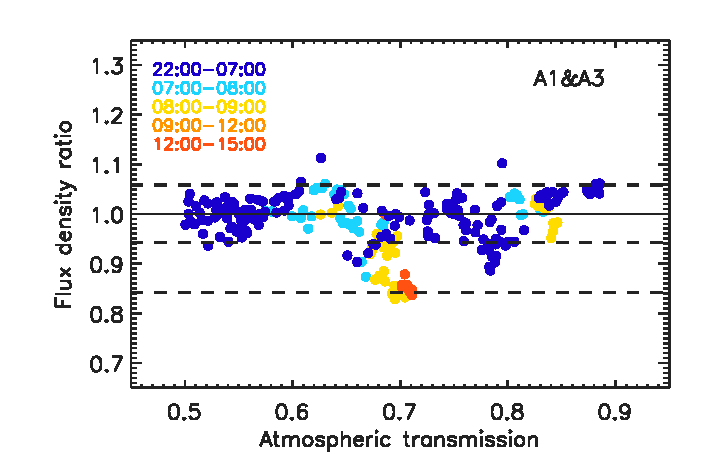
\includegraphics[clip=true, trim={0.9cm, 0, 0.5cm,
        0.6cm},width=0.45\linewidth]{Figures/NIKA2/plot_flux_density_ratio_obstau_allbright_obsdate_corrected_skydip_rescaled_1mm.pdf}
    \hfill
    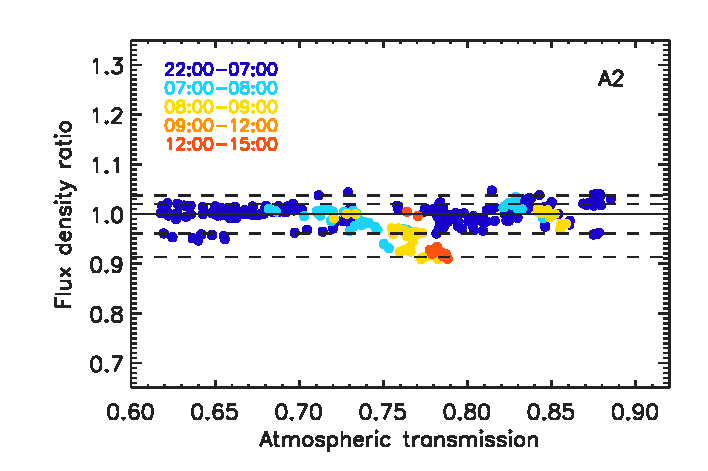
\includegraphics[clip=true, trim={0.9cm, 0, 0.5cm, 0.6cm},width=0.45\linewidth]{Figures/NIKA2/plot_flux_density_ratio_obstau_allbright_obsdate_corrected_skydip_rescaled_a2.pdf} 
    \caption[Baseline calibration rms error estimate]{Baseline
      rms calibration uncertainties. The
      measured-to-median flux density ratio of bright sources is
      plotted as a function of the atmospheric transmission
      color-coded according to the UT
      observation time of the scans for the combination of A1$\&$A3
      (top pannel)
      and for A2 (bottom pannel).
      The inner dashed lines from either sides of the
      unity-ratio line show the rms errors, which
      are less than 6\% at $1\,\rm{mm}$ and 3\% at $2\,\rm{mm}$, while
      the outer dashed lines show the $95\%$ confidence level contours.
      The lowest flux ratio data points correspond to some of the
      scans acquired during daytime between 8:00 UT and 15:00 UT
      hours (yellow and red), while the scans acquired during nighttime
      between 22:00 UT and 7:00 UT yield data points (dark blue)
      well distributed within the rms error with a few outliers.}
    \label{fig:allbright_rms_corrected_skydip}
  \end{center}
\end{figure}
%
\`A la figure~\ref{fig:allbright_rms_corrected_skydip}, nous
présentons les rapports de la densité de flux mesurée sur médiane,
après la calibration \emph{Baseline} et pour
le jeu de scans \emph{PS-800mJy} et testons leur stabilité en
fonction de la transmission atmosphérique, $\exp{-\taunu x}$. Les
rapports de flux sont compatibles avec l'unité  dans l'intervalle de
transmission atmosphérique testé et dans les deux bandes de fréquence,
indiquant l'absence d'effets systématiques significatifs après
correction de l'atténuation de l'atmosphère par la méthode décrite à
la Sect.~\ref{se:corrected_skydip}. Par ailleurs, nous observons un
groupe de scans pour lequel le rapport de flux est à la limite du
contour à 95\% de confiance. Un repérage des scans en fonction de
l'intervalle horaire auquel ils ont été observés (code de couleur)
nous indique que les scans concernés ont été observés soit le matin,
vers le lever du Soleil, soit en début d'après-midi, c'est-à-dire
proche des coupures sur l'heure UT, comme définies dans la sélection
\emph{Baseline}. Dit autrement, il serait possible de réduire encore
les incertitudes de calibration avec des coupures plus sévères, au
prix d'exclure davantage d'observations. Nous avons estimé que les
coupures \emph{baseline}, qui préservent 16 heures d'observation par
jour représentaient un bon compromis.

Dans la table~\ref{tab:Calibration_results_all}, nous rassemblons les estimations de l'erreur
de calibration RMS, basée sur $\sigma_\nu$, pour les différentes
méthodes de calibration discutées.
\begin{table*}[!htbp]
\begin{center}
\caption[Comparison of calibration results using three
  methods]{Erreur de calibration RMS en $\%$ pour trois méthodes de
  calibration : la méthode \emph{Baseline}
  (Sect.~\ref{se:corrected_skydip}), une méthode utilisant les opacités
atmosphériques dérivées des mesures du tau-mètre (Sect.~\ref{se:opacity_methods}) et une méthode utilisant une
correction photométrique (Sect.~\ref{se:afternoon_calibration}). La
première ligne indique le nombre de scans sélectionnés pour évaluer
les erreurs.} 
\label{tab:Calibration_results_all}
\begin{tabular}{lrrr}
  \hline\hline
  \noalign{\smallskip}
  \multicolumn{1}{c}{}  &  \multicolumn{3}{c}{Methods} \\\cline{2-4}
  \noalign{\smallskip}
  \multicolumn{1}{c}{Characteristics} &  \emph{baseline}  & {\small {\tt taumeter}}  & {\small {\tt PC-point}} \\
  \hline
  \noalign{\smallskip}
  $\#$ selected &   264    &    264   &  283 \\
  1mm           &   5.7    &    7.9   &  4.9 \\
  2mm           &   3.0    &    3.8   &  2.4 \\
\hline
\end{tabular}
\end{center}
\end{table*}

La méthode \emph{Baseline}, telle qu'elle est décrite à la
Sect.~\ref{se:corrected_skydip}, permet une mesure des densités de
flux avec une incertitude RMS $<6\%$ à 1\,mm et de $3\%$ à 2\,mm. Ce
résultat est remarquable pour une expérience millimétrique au sol,
pour lesquelles l'état de l'art de l'erreur RMS de calibration est
$\lesssim$ $10\%$ ~\citep{Dempsey2013_SCUBA2}. Il constitue une
validation de nos choix méthodologiques. La robustesse de la méthode
est également testée en comparant les résultats obtenus avec les méthodes
alternatives. Nous vérifions que la méthode \emph{Taumeter} est
associée à une dispersion légèrement supérieure des mesures de flux,
comme attendu (voir
Sects.~\ref{se:opacity_methods}~et~\ref{se:corrected_skydip}). En
revanche, la méthode \emph{PC-point} permet d'obtenir une erreur RMS
inférieure à l'erreur mesurée avec la méthode \emph{Baseline} tout en
incluant plus de scans. C'est un résultat encourageant pour les
méthodes fondées sur une correction photométrique. Toutefois, la
validation de telles méthodes requerrait encore de s'assurer du
contrôle des effets systématiques liés à l'estimation de
l'élargissement apparent du lobe (qui est réalisée par un suivi de la
FWHM sur les {\tt pointages} dans le cas de \emph{PC-point}). Au
contraire, les effets systématiques sont sous-dominants pour la
méthode \emph{Baseline}, comme discuté à la section suivante.

\subsection{L'incertitude de calibration absolue}
\label{se:syste}

L'erreur RMS constitue une estimation des incertitudes liées
aux conditions d'observation. Les erreurs de calibration incluent en
sus l'incertitude de calibration absolue et les erreurs
systématiques.  

Si l'incertitude sur la mesure des opacités
atmosphériques $\taunu$ est bien inclue dans l'erreur de calibration
RMS, l'incertitude sur le facteur correctif $a_\nu$ qui est appliqué
aux estimées de $\taunu$ contribue à l'erreur systématique. Nous
propageons l'incertitude sur $a_\nu$, évaluée à $\Delta a_\nu = 0.03$,
à l'erreur sur le flux, pour deux valeurs de l'opacité atmosphérique
le long de la ligne de visée. Pour les conditions atmosphériques de
référence du télescope de 30-m de l'IRAM, définies par une hauteur
de vapeur d'eau saturante (pwv) de 2\,mm et une élévation de
$60\degree$, correspondant à de bonnes conditions lors des semestres
d'hier, nous trouvons une incertitude sur les flux inférieure au
pour-cent dans les deux bandes de fréquence. Considérant les pires
conditions atmosphériques permises par la sélection de scan
\emph{Baseline}, l'erreur systématique sur les flux est au maximum de
$2\%$ à 1\,mm. De plus, ces erreurs sont évaluées pour le cas le plus
défavorable où la différence entre les conditions atmosphériques du
calibrateur primaire et de la source sont maximales. Elles représentent
des estimations pessimistes de l'erreur systématique liée à la
correction de $\taunu$.

Une autre source d'erreur systématique vient de la précision avec
laquelle sont connues les bandes passantes de NIKA2. Dans le cadre de
notre système photométrique, les densités de flux ne sont pas
intégrées dans les bandes passantes, mais données à une
fréquence de référence, ce qui minimise cette erreur
systématique. L'incertitude sur les bandes passantes se propage aux
flux uniquement pour les sources dont la densité spectrale d'énergie
diffèrent de celle du calibrateur primaire, via les corrections de
couleur. La caractérisation spectrale de NIKA2 en laboratoire à permis
une mesure des bandes passantes à mieux que 1\%. En utilisant cette
limite supérieure pour l'incertitude sur les bandes passantes, nous
trouvons une erreur sur les flux inférieure ou de l'ordre du pour-mille
pour la plupart des sources. 

L'incertitude de calibration absolue est donc dominée par
l'incertitude sur le modèle de densité de flux pour notre calibrateur
primaire, Uranus, qui est estimée à environ $5\%$
dans~\citet{Bendo2013} aux fréquences d'observation de NIKA2. Nous
annonçons donc une erreur systématique négligeable et une incertitude
de calibration absolue de $5\%$ dans les deux bandes de fréquence.





%----------------------------------------------------------------------------------------
%
%
%
%
%
%               Sensibilité
%
%
%
%
%
%----------------------------------------------------------------------------------------
\section{Sensibilité}
\label{se:sensibilite}


Nous caractérisons la sensibilité de NIKA2 en évaluant la densité de
flux équivalente au bruit (\emph{Noise Equivalent Flux Density},
NEFD). La robustesse de cette évaluation est testée en comparant les
résultats de différentes méthodes et en utilisant un vaste jeu de
données. \`A la Sect.~\ref{se:nefd_methodes}, nous présentons deux
méthodes d'estimation de la NEFD et comparons les résultats pour un
même jeu de données. Ensuite, à la Sect.~\ref{se:nefd_mesures}, nous
étudions l'évolution de la NEFD avec les conditions atmosphériques et
discutons l'implication de la NEFD mesurée sur les temps d'observation
requis pour obtenir une cartographie à une profondeur donnée. 


\subsection{Méthodes}
\label{se:nefd_methodes}

La NEFD correspond à l'erreur à $1\,\sigma$ que l'on mesure sur la
densité de flux pour une seconde d'intégration sur la source et à une
opacité atmosphérique nulle. Elle est donc reliée à l'erreur à
$1\,\sigma$ sur la densité de flux, notée $\Delta S_\nu$,  par
\begin{equation}
  \Delta S_\nu (t) = {\rm{NEFD}} \,\, e^{ \tau_{\nu} x}
  \frac{1}{\sqrt{t_{\rm{det}}(t)}},
  \label{eq:relation_sigma_nefd}
\end{equation}
où $t_{\rm{det}}$ est le temps d'observation pendant lequel au moins un
détecteur pointe sur la source. Ce temps dépend de la stratégie de
balayage de la source. Il est égal au temps d'observation réel, $t$,
si la source ne sort à aucun moment du champs de vue et que celui-ci
est rempli de détecteurs valides.

Nous avons développé deux méthodes pour estimer la NEFD. L'une,
appelée \emph{Deep Integration}, se base sur l'étude de l'évolution du
bruit dans les cartes de densité de flux, lors d'une observation
longue d'une source faible, tandis que l'autre, \emph{Scatter}, repose
sur l'extrapolation à opacité nulle d'un ensemble de mesures de NEFD
sur des scans individuels.
Pour \emph{Deep Integration}, nous construisons une série de cartes de
la densité de flux à partir d'une longue observation d'une même source, en
incluant de plus en plus de scans. Chaque scan est utilisé pour
produire une carte individuelle comme décrit à la
Sect.~\ref{se:overview_pipeline}. Puis ces cartes par scan sont
pondérées par l'inverse de leur variance et co-additionnées pour
construire la carte finale. Leur contribution relative à la
co-addition va donc dépendre de l'atténuation de l'atmosphère au
moment du scan. Cet effet est pris en compte lors du calcul du temps
d'intégration par détecteur pour la co-addition de $n$ scans, en
définissant un temps d'intégration effectif, $t_{\rm{eff}} (n)$, qui
inclut l'atténuation de l'atmosphère. Avec cette définition, 
l'Eq.~\ref{eq:relation_sigma_nefd} se ré-écrit
$\Delta S_\nu (n) = {\rm{NEFD}} / \sqrt{t_{\rm{eff}}(n)}$.
L'évolution de $\Delta S_\nu$ avec le nombre de scan $n$ est mesurée
directement dans la série de cartes de densité de flux, et la NEFD est
estimée en ajustant un modèle en $t^{-1/2}$ sur ces mesures.

La seconde méthode, $\emph{Scatter}$, consiste à mesurer directement
la NEFD sur la ligne de visée, NEFD$_{\taunu x}$ = NEFD $\exp{ \tau_{\nu} x}$, à partir
d'une carte de la densité de flux, en inversant
Eq.~\ref{eq:relation_sigma_nefd}. La source ciblée doit être peu
brillante, $<1\,$Jy, pour éviter que l'estimation de l'incertitude sur
le flux ne soit biaisée par le signal. En répétant une telle mesure
sur un grand nombre de scans acquis dans des conditions d'observation
diverses, nous pouvons vérifier l'évolution de la NEFD avec
l'atténuation atmosphérique. La NEFD est estimée en prenant la médiane
des mesures de la NEFD sur la ligne de visée, après correction de
l'atténuation de l'atmosphère.    

\begin{figure}[!thbp]
  \begin{center}
    \includegraphics[trim={0.5cm, 0, 0, 0.5cm}, clip, angle=0, width=0.495\textwidth]{Figures/NIKA2/hls_nefd_vst.eps}
    \includegraphics[trim={0.5cm, 0, 0.2cm, 0.5cm}, clip, angle=0, width=0.485\textwidth]{Figures/NIKA2/hls_NEFD_vs_TauElev_all.eps}
    \caption{Application de deux méthodes d'estimation de la NEFD à
      une longue observation de \hls. \`A gauche, l'erreur à 1\,$\sigma$
      sur la densité de flux est tracée en fonction du temps
      d'intégration effectif $t_{\rm{eff}}$ (voir le texte). Les
      droites en noir représentent les meilleurs ajustement d'un
      modèle en $t_{\rm{eff}}^{-1/2}$; leur amplitude donne une
      estimée de la NEFD. \`A droite, la NEFD mesurée sur
      la ligne de visée est tracée en fonction de l'opacité
      atmosphérique observée, $\taunu\,x$. Les courbes en noir
      montrent l'évolution attendue en $\exp{\taunu\,x}$, normalisée
      par la NEFD à atmosphère nulle. Dans les deux panneaux,
      l'analyse est effectuée pour la matrice  A1 (bleu clair), A3
      (bleu foncé), la combinaison A1\&A3 (bleu ciel), et A2 (rouge).}
    \label{fig:nefd_twomethods}
  \end{center}
\end{figure}
%
Nous comparons les résultats de ces deux méthodes sur un même jeu de
données à la Fig.~\ref{fig:nefd_twomethods}.
Pour cela, nous avons choisi une source assez faible,
\hls~\citep{Combes2012}, dont le flux attendu dans les bandes de NIKA2
est de quelques dizaines de mJy. Cette source a été observée en
effectuant des scans OTF $8' \times 5'$, pendant environ neuf heures,
lors de la campagne N2R9. Le panneau de gauche de la
Fig.~\ref{fig:nefd_twomethods} montre l'incertitude sur la densité
de flux en fonction du temps effectif d'intégration,
tandis que le panneau de droite présente la NEFD sur la ligne de
visée, NEFD$_{\taunu x}$, en fonction de l'opacité sur la ligne de
visée, $\taunu x$. Nous vérifions que l'incertitude sur le flux, pour
les matrices individuelles et pour la combinaison des matrices à 1\,mm,
diminue avec le temps d'intégration en $t^{-1/2}$ comme attendu. Nous
vérifions également l'évolution attendue de la NEFD$_{\taunu x}$ avec
l'atténuation de l'atmosphère. Finalement, les
estimées de la NEFD avec les deux méthodes, rassemblées dans la
table~\ref{tab:nefd_summary}, sont en accord à mieux que 7\%. Le
choix méthodologique a donc peu d'impact sur l'estimation de la
NEFD. Nous testons ensuite nos résultats et estimons les incertitudes
sur la NEFD en utilisant un plus grand jeu de données.  

%  comparison entre methods
\begin{table}[!htbp]
  \centering
  \caption[]{Tests de stabilité de la NEFD. Estimées de la NEFD
    en $\rm{mJy}.s^{1/2}$ obtenues en utilisant soit la méthode \emph{Deep
      Integration}, abrégée en Deep int., soit la méthode
    \emph{Scatter}, et pour deux jeux de données, l'observation longue de
    \hls\ et l'ensemble des scans vers des sources sub-Jy acquis lors
    des trois campagnes de référence. La dernière ligne du tableau
    donne les résultats pour la combinaison de tous ces scans (soit 202,
    481 et 430 scans lors de N2R9, N2R12 and N2R14, respectivement).}
  \label{tab:nefd_summary}
  \begin{tabular}{llrrrr}
    \hline\hline
    \noalign{\smallskip}
    Data set   & Method   & A1      &   A3    &   A1\&A3 &    A2 \\
    \noalign{\smallskip}
    \hline
    \noalign{\smallskip}
    \hls &     Deep int.  &  46.6  &    38.4  &    30.4  &   8.5  \\
    %   G2   &    $t^{-1/2}$  &  44.0  &    34.7  &    29.6  &  7.8  \\
         &     Scatter    &  45.7  &    36.3  &    28.5  &   8.2  \\
    \hline
    \noalign{\smallskip}
    N2R9     & Scatter    & 47.0 &  36.9  & 28.8  & 8.4 \\
    N2R12    &            & 47.3 &  36.4  & 30.2  & 8.5 \\
    N2R14    &            & 47.3 &  39.8  & 30.9  & 9.3 \\
    Combined &            & 47.2 &  37.9  & 30.1  & 8.8 \\
    \hline
  \end{tabular}
\end{table}

\subsection{Tests de robustesse aux conditions d'observation}
\label{se:nefd_mesures}

Nous utilisons la méthode \emph{Scatter}, qui est applicable à des
observations de sources variées, pour tester la robustesse de
l'estimation de la NEFD sur un vaste jeu de données. Ce jeu se compose
de l'ensemble des scans des trois campagnes de référence, vers des
sources de flux inférieur à 1\,Jy dans les deux bandes de fréquence,
et respectant les critères de sélection \emph{Baseline}. Il comprend
plus d'un millier de scans. \`A la
figure~\ref{fig:nefdvsbackground_below_1Jy}, nous traçons la NEFD sur
la ligne de visée, NEFD$_{\taunu x}$ , en fonction de l'opacité
atmosphérique observée, $\taunu x$, en distinguant les scans par
campagnes d'observation. Les courbes ne résultent pas de l'ajustement
d'un modèle mais représentent l'évolution attendue avec l'atténuation
de l'atmosphère, normalisée par la NEFD à atmosphère nulle. Nous
vérifions ainsi que la NEFD$_{\taunu x}$ varie comme attendu avec le
"bruit du ciel'', pour une grande gamme de conditions d'observation. De
plus, nous mesurons des NEFD$_{\taunu x}$ compatibles pour les trois
campagnes de référence. Les valeurs de la NEFD estimées pour chaque
campagne et pour l'ensemble du jeu de données sont compilées dans la
Table~\ref{tab:nefd_summary}. Nous évaluons l'incertitude sur la NEFD
en calculant la rms des mesures de NEFD$_{\taunu x}$ corrigées de
l'atténuation de l'atmosphère. Nous trouvons une erreur rms de
3\,mJy.s$^{1/2}$ à 1\,mm et 1\,mJy.s$^{1/2}$ à 2\,mm, en accord avec la
dispersion des estimées de la NEFD données à la
Table~\ref{tab:nefd_summary}. En utilisant l'estimation sur l'ensemble
des scans, nous annonçons une NEFD de $30 \pm 3$\,mJy.s$^{1/2}$ à 1\,mm
et de  $9 \pm 1$\,mJy.s$^{1/2}$ à 2\,mm. Par ailleurs, nous constatons
une moindre sensibilité de la matrice A1 comparée à A3, que nous
interprétons comme l'impact du défaut de transmission avéré de la lame
dichroïque (Sect.~\ref{se:gains}).
%
\begin{figure}[!thbp]
\begin{center}
  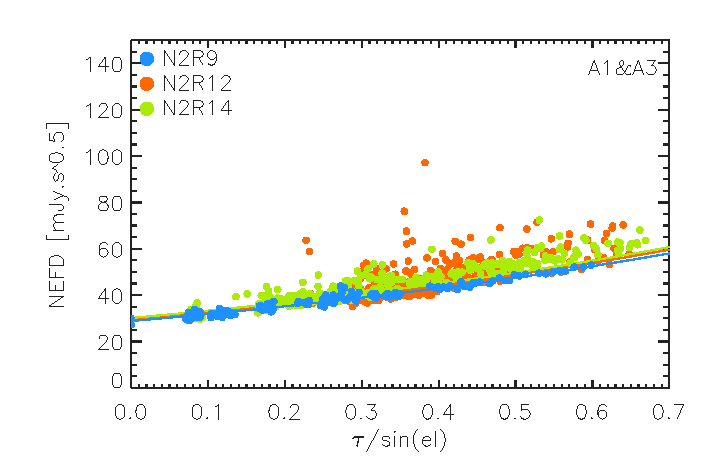
\includegraphics[clip=true,width=0.47\textwidth]{Figures/NIKA2/plot_nefd_vs_obstau_corrected_skydip_vfinal_1mm.pdf}
  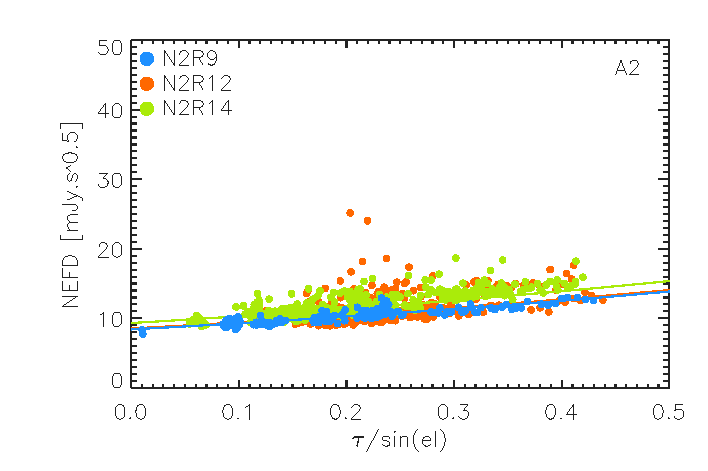
\includegraphics[clip=true,width=0.47\textwidth]{Figures/NIKA2/plot_nefd_vs_obstau_corrected_skydip_vfinal_a2.pdf}
  \caption{\'Evolution de la NEFD avec les conditions
    d'observation. La NEFD le long de la ligne de visée, NEFD$_{\taunu
    x}$, est tracée en fonction de l'opacité atmosphérique observée,
    $\taunu\,x$, dans la bande à $1\,\rm{mm}$ (à gauche) et à
    $2\,\rm{mm}$ (à droite). Les points de données correspondent aux
    estimées de NEFD$_{\taunu x}$ en $\rm{mJy}\cdot s^{1/2}$ obtenues
    lors des campagnes N2R9 (en bleu), N2R12 (orange) and N2R14
    (chartreuse). Les courbes représentent l'évolution attendue de la
    NEFD sur la ligne de visée en fonction du "bruit du ciel'',
    normalisée par l'estimée de la NEFD à atmosphère nulle.}
  \label{fig:nefdvsbackground_below_1Jy}
\end{center}
\end{figure}


Nous évaluons aussi la vitesse de cartographie (\emph{Mapping Speed}), 
définie comme la zone du ciel $\mathcal{A}_{\rm{scan}}$ qui peut être
observée à un niveau de bruit $\Delta_\sigma$ of $1\,\rm{mJy}$ en un
temps d'intégration $\Delta_t$ de une heure. En notant $d_{\rm{FOV}} =
6.5\,\rm{arcmin}$ le diamètre du champ de vue et $\eta$ la fraction de
KID valides (Sect.~\ref{se:fov_geometry}), la vitesse de cartographie
$M_{\rm{s}}$ s'écrit: 
\begin{equation}
M_{\rm{s}} = \frac{\mathcal{A}_{\rm{scan}}}{\Delta_\sigma\Delta_t} = 
\eta \, \frac{\pi}{4} d_{\rm{FOV}}^2 \, \frac{1}{\rm{NEFD}^2}\, ,
\label{eq:mapping_speed}
\end{equation}
et s'exprime en arcmin$^2 \cdot \rm{mJy}^{-2} \cdot
\rm{h}^{-1}$. C'est cette quantité qui est utilisée pour calculer
les temps d'observation. Ainsi, le temps d'observation nécessaire pour
atteindre le niveau d'incertitude sur les densités de flux
$\sigma_{obs}$ souhaité, sur une certaine couverture du ciel
$\mathcal{A}_{\rm{scan}}$, et en supposant une opacité atmosphérique
  sur la ligne de visée $\taunu x$ est
\begin{equation}
  t_{\rm{obs}} = \frac{\mathcal{A}_{\rm{scan}}}{ M_{\rm{s}}} \, \left(\frac{e^{\taunu\, x}}{\sigma_{obs}}\right)^2.
\end{equation}
\`A partir de l'estimation de la NEFD, nous dérivons une vitesse de
cartographie de $111 \pm 11$ et $1388 \pm 174$ arcmin$^2 \cdot
\rm{mJy}^{-2} \cdot \rm{h}^{-1}$ respectivement à 1 et
2\,mm. Ce résultat remarquable situe NIKA2 parmi les meilleurs
instruments millimétriques de cartographie haute-résolution d'un grand
champ de vue~\citep{Tony2019}.



%----------------------------------------------------------------------------------------
%
%   
%
%----------------------------------------------------------------------------------------
\chapter{Résumé des performances}
\label{chap:nika2_resume}
%\chapter{Résumé des performances}

Ce chapitre vient clore la partie de ce document consacrée au
\emph{commissioning} de NIKA2 et la caractérisation de ses
performances.
L'essentiel du travail d'analyse a été réalisé sur une période
d'environ deux ans, entre septembre 2016, soit après l'intervention
majeure sur l'instrument, et décembre 2018. En septembre 2017, la
revue des performances de NIKA2 par l'IRAM a
marqué la fin de la phase de \emph{commissioning} en intensité, et la
livraison de l'instrument a été parachevée en décembre 2018 avec la
remise d'un document détaillant la calibration et la caractérisation des
performances.

Responsable de la caractérisation des performances de NIKA2 depuis
septembre 2016, j'ai dirigé toutes les phases de ce travail, jusqu'à
sa concrétisation par la remise du document à l'IRAM et l'écriture de
l'article de référence~\citep{Perotto2019}. Cette activité
d'encadrement a été rythmée par l'organisation des réunions du
consortium NIKA2, d'abord hebdomadaires puis bi-mensuelles; la création et
l'animation de la \emph{Commissioning Tiger Team}, au sein de laquelle
a été réalisée la caractérisation des performances; la présentation
des performances lors de la revue de l'IRAM; la formation d'une
personne de l'IRAM à la calibration \emph{Baseline}; la coordination
de l'écriture du document \emph{Commissioning\&Performance}, puis celle
de l'article. Il s'agit de l'expérience d'encadrement de la recherche
la plus complète que j'ai effectuée jusque-là.    

Parmi nos réalisations les plus marquantes, deux ont vocation à avoir
un impact important. La première est la méthode de calibration de
référence que nous avons développée pour NIKA2, lui assurant
robustesse aux effets systématiques et stabilité aux conditions
d'observation. Ensuite, l'article détaillant nos méthodes et nos
résultats vise à faire référence pour les utilisateurs de NIKA2 et
pour la calibration de futurs instruments millimétriques, en
particulier utilisant la technologie des KID.

Ici, nous résumons les principaux résultats décrits dans cet article,
tels qu'ils ont été détaillés au chapitre précédent, puis nous
proposerons quelques pistes d'amélioration des performances de
NIKA2 pour le futur.  


\section{Les performances}

Les performances de NIKA2 au télescope de 30-m de l'IRAM ont été
caractérisées à partir d'un vaste ensemble d'observation de sources de
calibration, de sources de pointage et de sources faibles, effectuées
lors de trois campagnes d'observation réparties au cours d'une année. Cet
ensemble forme un échantillon répésentatif des conditions
d'observation sur le site.

La caractérisation des performances repose sur une calibration de
référence, la calibration \emph{Baseline}, que nous avons développée
et extensivement testée. Cette calibration est fondée sur quatres
choix méthodologiques principaux. La soustraction du bruit corrélé des
détecteurs repose sur une méthode de décorrelation de \emph{modes
  communs} mesurés dans les données, qui a été largement testée pour
le traitement des sources ponctuelles. Le flux des sources ponctuelles
est mesuré par l'ajustement d'une gaussienne de référence de FWHM fixe
et pour une fréquence de référence. L'attenuation de l'atmosphère est
corrigée en utilisant une version modifiée de la méthode employée dans
NIKA~\citep{Catalano2014}, basée sur la mesure de l'opacité
atmosphérique par les KID. L'élargissement apparent du
lobe de l'instrument, lié aux variations de température extérieure,
est traité par une sélection des scans retenant 16 heures
d'observations par jour.

Les performances sont définies par l'évaluation d'un ensemble de
caractéristiques instrumentales. Les principaux résultats de cette
mesure sont regroupés dans le tableau~\ref{tab:nika2summary} et
résumés ci-dessous.

\begin{table}[!thbp]
  \caption{Résumé des principales caractéristiques instrumentales de NIKA2}
  \label{tab:nika2summary}
  \centering    
  \begin{tabular}{rrrcl}
  \hline\hline
  \noalign{\smallskip}
  & Array 1\&3 & Array 2 & & Commentaire \\
  \noalign{\smallskip}
  \hline
  \noalign{\smallskip}
  Fréquence de référence [GHz]  & 260  & 150   &  & \footnotesize{voir Sect.~\ref{se:systeme_photo}}  \\
  Fréquence centrale [GHz]      &  254.7\&257.4  & 150.9 &  & \footnotesize{à atmosphère nulle}   \\
  Largeur de bande passante  [GHz]     &   49.2\&48.0   & 40.7  &  & \footnotesize{à atmosphère nulle} \\
  \hline
  \noalign{\smallskip}
  Diamètre du champ de vue     [arcmin] &   6.5       &   6.5   &  &  \\  
  Nombre total de détecteurs            &  1140\&1140 &    616  & & \footnotesize{voir Sect.~\ref{se:matrices}}\\
  Fraction de détecteurs valides [$\%$] &  84         &     90  & & \footnotesize{voir Sect.~\ref{se:KID_selection}} \\
  Echantillonage du champ de vue \hspace{3mm} [$\lambda/D$] & 1.1 &  0.87 & & \footnotesize{voir Sect.~\ref{se:KID_pointing}} \\
  \hline
  \noalign{\smallskip}
  FWHM de référence\hspace{3mm} [arcsec]          & $12.5$     &   $18.5$  &  & \footnotesize{voir Sect.~\ref{se:systeme_photo}}\\
  FWHM$^c$\hspace{3mm} [arcsec]    &  $11.1 \pm 0.2$  &  $17.6 \pm 0.1$  & & \footnotesize{voir Sect.~\ref{se:mainbeam}}\\
  Efficacité du lobe principal \hspace{3mm} [$\%$] &  $55 \pm 3$   &  $77 \pm 2$  &  & \footnotesize{calculée jusqu'à 180''}\\
  Dispersion de la FWHM [arcsec]  &    0.6        &      0.6        & & \footnotesize{\citet{Adam2018}} \\
  \hline
  \noalign{\smallskip}
  Erreur de calibration absolue [\%]      &   5         & 5 & &  \footnotesize{voir Sect.~\ref{se:syste}}\\
  Erreur de calibration systématique\hspace{3mm}  [\%]      &    0.6        & 0.3 & & \footnotesize{pwv = 2\,mm, $\elev = 60\degree$} \\
  Erreur de calibration RMS [\%]          &   5.7       &     3.0       & & \footnotesize{voir Sect.~\ref{se:rms_error}} \\
  Erreur de pointage    [arcsec]          & $<3$ &  $<3$  & & \footnotesize{\citet{Greve1996}} \\
  \hline
  \noalign{\smallskip}
  NEFD \hspace{3mm} [$\rm{mJy} \cdot \rm{s}^{1/2}$]  & $30 \pm 3$  & $9 \pm 1$ &  & \footnotesize{voir Sect.~\ref{se:nefd_mesures}}\\
  M$_{\rm{s}}$\hspace{3mm} [arcmin$^2 \cdot
    \rm{mJy}^{-2} \cdot \rm{h}^{-1}$] & $111 \pm 11$  &  $1388 \pm 174$ &  & \footnotesize{\emph{Mapping speed}}\\
  \hline
  \end{tabular}
\end{table}

Les 2900 KID qui composent les matrices de NIKA2 détectent un signal
astrophysique au moins lors de certaines observations. Nous
définissons des critères pour sélectionner les KID les plus
stables. Nous trouvons une fraction de KID valides (utilisables pour
l'exploitation scientifique) de 84\% dans la bande à 1\,mm et 90\% à
2\,mm. Les détecteurs non-sélectionnés se répartissent aléatoirement
dans le plan focal, de sorte que le champ de vue de 6,5' de diamètre
est bien couvert. \`A partir de la taille réel des détecteurs
(2.75\,mm et 2.0\,mm) et du diamètre de la pupille d'entrée (27\,m),
nons trouvons une taille des détecteurs en unité d'échantillonage du
lobe de 1,1 et 0,9 $\lambda$/D dans les bandes à 1 et 2\,mm.   

Le lobe principal est bien modélisé par une gaussienne de FWHM
17,6''$\pm$0,1'' à 150\,GHz et 11,1''$\pm$0,2'' à 260\,GHz. Son
efficacité mesurée jusqu'à une distance radiale de 180'' est de
77$\pm$2\% et 55$\pm$3\% à 150 et 260\,GHz, respectivement. Une
fraction significative du signal est donc reçue au-delà du lobe
principal, dans la structure complexe, formée de lobes d'erreur et
diverses figures de diffraction, du lobe total. La dispersion de la
FWHM dans le champ de vue a été mesurée dans~\citet{Adam2018} à partir
de carte individuelle par détecteur. Elle est de 0,6'' dans les deux
canaux de fréquence, en accord avec la dispersion attendue d'après la
mesure des surfaces focales (voir Sect.~\ref{se:focus}).   

\`A partir d'un large échantillon de scans de sources
brillantes, bien représentatif des conditions d'observation au
télescope de 30-m, nous vérifions la stabilité des mesures de flux aux
conditions d'observation et évaluons l'erreur de calibration RMS. Nous
trouvons environ 3\% à 150\,GHz et 6\% à 260\,GHz. Ces résultats
indiquent une stabilité remarquable pour un instrument millimétrique
au sol et valident les choix méthodologiques de notre
calibration. Pour évaluer l'incertitude de calibration, l'erreur RMS
doit être combinée à l'erreur de calibration absolue, qui est de 5\%
dans les deux bandes, et à l'erreur systématique. La contribution
dominante à l'erreur systématique est l'incertitude sur le facteur
correctif appliqué aux mesures d'opacité atmosphérique. \'Evaluée pour
les conditions d'observation d'hiver de référence de l'IRAM (pwv=2\,mm
et $\elev = 60\degree$), cette erreur est inférieure au pourcent dans
les deux bandes.

\`A partir d'observations longue durée d'une source faible, nous avons
vérifié que le bruit sur le flux diminuait comme l'inverse de la
racine carré du temps d'intégration. La sensibilité de l'instrument a
été évaluée en comparant les résultats de deux méthodes et en
utilisant un échantillon de plus de 1000 scans, afin de
tester sa robustesse aux choix d'analyse et aux conditions
d'observation.
Nous trouvons une densité de flux équivalente au bruit (NEFD) de
$9\pm1$\,mJy.s$^{1/2}$ à 150\,GHz et de $30\pm3$\,mJy.s$^{1/2}$ à
260\,GHz. \`A partir de ces estimations, nous avons dérivé la vitesse
de cartographie (\emph{mapping speed}), c'est-à-dire la zone du ciel
qui peut être cartographiée à une profondeur de 1\,mJy en une heure
d'intégration. Nous trouvons une \emph{mapping speed} de 1388$\pm$174
et 111$\pm$11 arcmin$^2$/mJy$^2$/h à 150 et 260\,GHz. Ces capacités de
cartographie placent NIKA2 parmi les meilleures instruments
millimétriques haute résolution de sa génération~\citep{Tony2019}.


%Les observations de NIKA2 devraient susciter des avancées
%significatives dans plusieurs domaines de l'astrophysique et la cosmologie.

\section{Perspectives d'amélioration}

NIKA2 satisfait tous les critères de performance requis par l'IRAM et
conditionnant son installation définitive au télescope de 30-m. Pour
certaines caractéristisques, l'objectif ambitieux vers lequel tendre,
après des améliorations successives, est déjà atteint, voire
surpassé. C'est le cas de la sensibilité dans le canal d'observation à
150\,GHz. Par exemple, une carte à 150\,GHz, couvrant tout le champ de
vue et à une profondeur de quelques centaines de $\mu$Jy peut être
obtenue en une heure de temps d'observation. Ce canal de fréquence
bénéficie d'une combinaison de conditions favorables, allant d'une plus grande
facilité de construction des matrices de KID à un moindre impact de
l'opacité atmosphérique, en passant par de meilleures performances du
système optique jusqu'au miroir primaire du télescope. Ainsi NIKA2 est
un instrument idéal pour cartographier l'émission diffuse à 150\,GHz
(e.g. les amas de galaxies via l'effet Sunyaev-Zel'dovich). En
revanche, la situation s'inverse dans la bande à 260\,GHz, où se
cumulent les facteurs limitants. Ainsi, la sensibilité à 260\,GHz est
juste acceptable, avec une RMS du bruit dans le champ de vue d'environ
0.7\,mJy en une heure d'observation dans les conditions de référence
de l'IRAM. Plusieurs pistes d'amélioration existent, dont certaines
font d'hors et déjà l'objet de développements. Ces améliorations
concernent le dispositif instrumental, la connaissance de l'instrument
et la méthode de calibration, et la méthode d'analyse des données.

\subsubsection{Améliorations instrumentales}

Le principal facteur limitant la sensibilité à 260\,GHz est la
transmission sous-optimale de la lame dichroïque qui affecte
principalement la composante de polarisation illuminant la matrice A1
mais a aussi un impact sur la matrice A3 (voir
Sect.~\ref{se:gains}). Des développements sont en cours à Cardiff pour
fournir les lames dichroïques combinant grande taille et haute
performance nécessaires à NIKA2 et aux futurs instruments
millimétriques. En parallèle, la construction d'un banc test, incluant
un système optique refroidi à environ 100\,mK, est prévue à Grenoble.

Les bandes passantes des matrices à 1\,mm sont actuellement limitées à
la zone centrale de la fenêtre permise par l'atmosphérique, leur
conférant une robustesse aux variations des conditions atmosphériques.  
Cette caractéristique permet à NIKA2 d'effectuer des observations
exploitables à 260\,GHz même dans des conditions atmosphériques
défavorables, aux prix d'une réduction de la sensibilité dasn ce
canal. Des matrices à 1\,mm acceptant une bande passante plus
large ont été développées à l'Institut Néel. 

La bande fréquencielle de l'électronique de lecture NIKEL-AMC limite
le nombre de KID qui peuvent être connectés à une même ligne de
base. Une nouvelle électronique est en cours de développement au LPSC
afin de doubler la largeur de bande. Cette nouvelle capacité pourrait
être exploitée de plusieurs manières : réduire la taille des KID des
matrices à 1\,mm pour un meilleur échantillonage du champ de vue et à
la clef, un gain en résolution angulaire, espacer les fréquences de
résonance des KID afin de réduire la diaphonie et \emph{in fine}
augmenter le nombre de détecteurs utilisables, résoudre le problème de
diminution du gain des détecteurs en fonction de leur place dans la
bande fréquentielle. 

NIKA2 bénéficierait également d'améliorations du télescope de
30-m. Une rénovation de la surface du miroir primaire limiterait
l'effet d'élargissement apparent du lobe dù aux variations de
température externe. Elle se traduirait aussi par une meilleure
efficacité du lobe principal à 260\,GHz, ce qui contribuerait à
améliorer la sensibilité. 

\subsubsection{Améliorations de la calibration et l'analyse}

Suite aux interventions sur l'instrument et aux améliorations
apportées pendant la période de commissioning, les bandes passantes
ont pu légèrement varier par rapport à celles du dispositif
instrumental avant l'installation au télescope, telles qu'elles
avaient été précisément mesurées au laboratoire. Les bandes passantes
sont actuellement en cours de caractérisation \emph{in situ} au moyen
d'un interféromètre Martin-Pupplett dédié, construit à l'Institut
Néel, et venant se placer devant la fenêtre d'entrée du
cryostat. Cette caractérisation précise permettra de réduire les
incertitudes liées aux corrections de couleur sur les
densité de flux. Plus indirectement et avec sans doute plus d'impact
encore, elle permettra de simuler l'effet de l'atmosphère intégré dans
les bandes passantes à partir de modèles physiques de type
ATM~\citep{Pardo2001, ATM}. Ces simulations, ainsi que la possibilité
d'extrapoler les mesures issues du tau-mètre résident aux fréquences
de NIKA2, seront cruciales pour tester nos méthodes d'estimation de
l'opacité atmosphérique pour chaque scan. \`A la clef, l'objectif est
d'améliorer la méthode \emph{skydip} pour l'estimation de l'opacité
atmosphérique, afin d'obtenir des densités de flux robustes à
l'atténuation de l'atmosphère, sans avoir recours à un facteur
correctif.

La déformation résiduelle du miroir primaire sous l'effet de son poids
a un impact sur le flux dépendant de l'élévation à laquelle il
observe. Cet effet est connu sous le nom de corrélation
gain-élévation~\citep{Greve1998b}. Une mesure plus précise de
l'atténuation atmosphérique, elle aussi dépendante de l'élévation, 
permettrait de mesurer l'effet gain-élévation avec une précision
suffisante pour corriger les densités de flux, améliorant encore
l'erreur RMS de calibration.

Une autre piste d'amélioration de la calibration concerne les
lobes. En particulier, la mesure du lobe total pourrait être étendue
au delà de 180''. Pour cela, deux methodes sont
envisageables. Une observation dédiée vers une source compacte très
brillante, telle Mars, dans des conditions d'observation favorables,
permettrait de construire une carte étendue sans soustraction de
l'atmosphère et donc avec un filtrage minimale des grandes échelles
angulaires. La deuxième piste requièrerait le développement de
méthodes de traitement du bruit corrélé qui préservent le signal aux
plus grandes échelles angulaires.


Plus généralement, l'amélioration de la décorrélation du bruit et la
caractérisation fine des effets de filtrages spatiaux constituent des
développements cruciaux et prioritaires de l'analyse de données. Là
encore, plusieurs pistes sont à l'étude, dont certaines mobilisent
déjà d'importants efforts. C'est le cas des méthodes visant à
l'amélioration du \emph{template} soustrait au signal de chacun des
détecteurs~\citep{Ponthieu2020}. Par exemple, dans \citet{Ruppin2019},
chaque \emph{template} résulte d'une combinaison d'un mode commun par
matrice, d'un mode commun par sous-bandes électroniques et d'une
composante dépendante de la tragectoire effectuée par le détecteur sur
le ciel. Une autre piste actuellement explorée consiste à adapter des
méthodes existantes de fabrication de cartes aux observations de
NIKA2. Par exemple, une version dédiée à NIKA2 de
\emph{Scanamorphos}~\citep{Roussel2013, Roussel2018}, un outil de
correction du bruit basse-fréquence ou \emph{destriage} est
actuellement en cours de tests. Enfin, une réflexion est menée pour
développer des méthodes de type \emph{destrieur} spécifiques pour les
observations avec des KID.

\section{Conclusion}
Les performances de NIKA2 sont conformes aux attentes
et exceptionnelles pour certaines (sensibilité à 150\,GHz). Ces
performances ont motivé la décision de l'IRAM de
l'ouverture de NIKA2 à la communauté scientifique dès octobre 2017.
Il enregistre déja 18 campagnes d'observation scientifique et restera
un instrument à demeure du télescope de 30-m de l'IRAM pour
au moins une décennie. L'exploitation scientifique a d'hors et déjà
commencée.

NIKA2 installé au 30-m de l'IRAM est actuellement l'unique opportunité
pour cartographier un champ de vue aussi large (6,5'' de diamètre) à
une résolution angulaire aussi fine (mieux que 18'') et simultanément
dans deux bandes de fréquence du domaine millimétrique. Il offre donc
une vue sans précédent sur l'univers millimétrique. Ainsi, il fournira
des observations critiques, aussi bien aux échelles planétaires et
galactiques qu'à hauts \emph{redshifts}, pour permettre des avancées
majeures dans de nombreux domaines de l'astrophysique et la
cosmologie~\citep[e.g.]{Rigby2018, Bracco2017, Bethermin2017, Mancuso2016,
  Ruppin2019a}.
%Par exemple, les observations de NIKA2 seront clef pour
%quantifier l'impact de l'environment sur les propriétés de la
%poussières et le processus de formation planétaire, pour comprendre la
%formation stellaire et sonder son évolution à toutes les époques, pour
%améliorer notre connaissance de la formation des structures à grande
%échelle et leur évolution à travers les ages cosmiques et sonder
%l'univers avec les amas de galaxies.   


NIKA2 est actuellement le meilleur instrument millimétrique pour la cartographie
haute-résolution des amas de galaxies à redshifts intermédiaires à
élevés ($z\in[0.5, 0.9]$) via l'effet Sunyaev-Zel'dovich. Son champ de
vue englobe un lobe de \emph{Planck}, tandis que sa résolution
angulaire est 17 fois meilleure. En alliant une haute résolution
angulaire et une grande vitesse de cartographie, il permet la
caractérisation des amas depuis leur coeur jusqu'à leur
périphérie. Les deux bandes de fréquence permettent de capturer
la signature spectrale de l'effet SZ pour une séparation
efficace des contaminants : la bande à 150\,GHz inclut le
maximum du signal SZ négatif, tandis que la bande à 260\,GHz mesure un
signal SZ très légèrement positif. L'exploitation des données de NIKA2
pour l'étude des amas de galaxie en tant que sonde cosmologique
constituera une importante partie de mon activité de recherche dans les
années à venir. La thématique de la cosmologie avec les amas de
galaxie, au coeur de mon projet de recherche, sera détaillée dans la
dernière partie de ce manuscript.



%----------------------------------------------------------------------------------------
%
%
%
%     PARTIE III: Cosmologie avec les amas
%
%     10 pages
%
%
%
%----------------------------------------------------------------------------------------

\part{Cosmologie avec les amas de galaxies dans NIKA2 et \emph{Euclid}}

%----------------------------------------------------------------------------------------
%
%   COSMO AVEC LES AMAS
%
%----------------------------------------------------------------------------------------
\chapter{Cosmologie avec les amas de galaxies}
\label{se:cosmo_general}
%\chapter{Cosmologie avec les amas de galaxies}
%\label{se:cosmo_general}

%----------------------------------------------------------------------------------------
%
%
%
%
%                COSMO-AMAS
%                 
%
%
%
%----------------------------------------------------------------------------------------

\emph{La cosmologie avec les amas de galaxies occupe une place centrale de
mon projet de recherche à court et moyen termes. Je commence la
seconde partie de ce manuscrit par un résumé succint de ce domaine,
qui n'a pas vocation à constituer une revue mais a deux
objectifs. D'abord, dans le cadre d'une mobilité thématique depuis
l'effet de lentille sur le CMB aux amas de galaxies, l'exercice a son
intérêt propre. Ensuite, ce résumé constitue l'introduction, fournit
la justification et situe le contexte de mon projet de recherche.}\\


Les amas de galaxies forment une puissante sonde cosmologique.
Ce sont les objets les plus massifs résultant du processus de formation
hiérarchique des structures à partir des maxima de
densité dans la distribution de matière primordiale. Ils contiennent
donc l'information sur les conditions initiales, le contenu et
l'évolution de l'Univers. Ce sont des traceurs aussi bien de la
distribution des grandes stuctures de l'univers que de leur
croissance~\citep[pour une revue]{Allen2011}. En mesurant une quantité
standardisable, telle la fraction de gaz qu'ils contiennent, les amas
sont utilisés pour mesurer les distances et ainsi sonder
l'histoire de l'expansion de l'Univers~\citep{Sasaki1996, Ettori2009}.  
L'abondance des amas et leur distribution spatiale sont sensibles en
particulier à la densité de matière $\Omega_{\rm{m}}$ et à l'amplitude
des fluctuations linéaires de densité spatialement moyennées sur un
rayon de 8\,Mpc\,$h^{-1}$, $\sigma_8$. Combinées
avec une sonde de l'univers primordial, tel le CMB, elles vont
permettre de contraindre les extensions du modèle
$\Lambda$CDM standard qui affectent la croissance des structures, dans
le secteur des neutrinos~\citep{Wang2005, Bolliet2019}, de l'énergie
noire~\citep{Haiman2001} ou des modifications de la
gravité~\citep{Mohr2003, Hagstotz2019}. Combiner le CMB et
la distribution d'amas de galaxie,
c'est aussi un formidable test de cohérence du modèle cosmologique.%,
%qui est alors
%contraint avec les deux extrêmes de la formation hierarchique des
%structures.
Le modèle doit décrire aussi bien la distribution des perturbations de
densité qui laissent leur empreinte sur le rayonnement émis au
découplage que la distribution statistique et spatiale des plus gros
objets qui se forment aux maxima de cette distribution de matière
initiale, à l'issu d'un long processus d'effondrement gravitationnel
dans un univers en expansion. 

\section{Des objets multi-sondes}
\label{se:multisondes}

Les amas de galaxies sont des objets gravitationnellement liés et
virialisés, dominés par la matière noire, qui représente environ 80\%
de leur contenu. Ce sont donc des halos de matière noire de
masse entre $10^{14}$ et $10^{15}$\,M$_{\odot}$, qui ont piégé du gaz,
chauffé ($\approx 10^{8}\,\rm{K}$) et ionisé, et des galaxies. Ce
plasma diffus, chaud et magnétisé domine
le contenu baryonique des amas, le milieu
intra-amas, représentant environ 17\% de la masse totale, tandis que
les galaxies constituent les 3\% restants. Gravitationellement
relaxés, ce sont des objets auto-similaires, décrits les uns par
rapport aux autres par des relations d'échelle. S'ils sont dominés par
des processus gravitationnels, ils sont aussi le lieu de processus
physiques baryoniques complexes, dont la plupart sont encore
imparfaitement compris, tels la formation des galaxies, le
refroidissement du gaz, le rôle de la rétro-action des supernovae et
noyaux actifs de galaxies (voir par exemple, \citet{Voit2005}). 

\'Etant multi-composantes, ils sont de façon inhérente multi-sondes.
La lumière stellaire des galaxies et la lumière diffuse du
milieu intra-amas sont détectables dans l'optique et l'infrarouge (IR)
proche. Dans ce domaine de longueur d'onde, les amas de galaxies sont
revélés par la distribution des galaxies qu'ils enferment, leur
dispersion de vitesse et le profil de luminosité du milieu
intra-amas. Leur potentiel gravitationnel intégré sur la ligne de
visée peut être reconstruit en exploitant les effets de lentille
gravitationnelle fort et faible sur la lumière des galaxies situées en
arrière-plan~\citep[ pour une revue]{Bartelmann2010}. Dans le domaine des
rayons X, le milieu intra-amas est détectable par l'effet Bremsstrahlung des
électrons et les raies d'émission des éléments plus lourds que
l'hydrogène~\citep{Sarazin1986} La densité électronique du milieu intra-amas peut être
cartographiée par photométrie en rayon X, tandis que la température
électronique peut être inferrée par spectroscopie. Dans le domaine
millimétrique, les amas de galaxies sont détectés par effet
Sunyaev-Zel'dovich, qui décrit la distortion spectrale induite par la
diffusion Compton inverse des photons du CMB sur les électrons du milieu
intra-amas~\citep{SZ1970}.
L'effet de lentille gravitationelle de l'amas sur les photon du CMB
laisse aussi une signature dans les cartes des anisotropies du
CMB~\citep{Seljak2000}. Finalement, les amas émettent par des
processus non-thermiques dans les domaines radio, ainsi que parfois
dans les domaines X énergétique (\emph{Hard X-ray}) et gamma, via les
phénomènes violents (supernovae, AGN, chocs) qu'ils
abritent~\citep{Rephaeli2008}.

Le caractère multi-composantes et complexe des amas est à la fois une
difficulté, car leur exploitation en cosmologie ne peut pas faire
l'économie de mesurer l'impact de ces processus et de leur évolution
sur les observables cosmologiques, et à la fois une force, car ces
observables sont multiples et peuvent etre combinées dans une analyse
cosmologique conjointe.

\section{Exploitation des amas de galaxies pour la cosmologie}
\label{se:sondecosmo}

Réprésentant les plus grands halos de matière noire formés
relativement récemment à l'échelle cosmologique ($0<z<3$), les amas de
galaxies dévient encore peu du régime linéaire de croissance des structures.
Leur croissance non-linéaire et sa dépendence au modèle cosmologique
est formalisée dans le cadre d'un modèle de halos~\citep[, par exemple
  pour une revue]{Cooray2002}. La fonction de masse des halos,
c'est-à-dire leur densité numérique par intervalle de masse et de
redshift, ainsi que les propriétés statistiques de leur distribution
spatiale, en particulier la fonction d'autocorrélation des halos, et
de leur distribution de vitesse encodent l'information
cosmologique. Des modèles analytiques de la fonction de masse des
halos ont été dérivés dans le cas sphérique~\citep{Press-Schechter1974}
et elliptique~\citep{Sheth2001}. Pour mieux capturer les effets
non-linéaires et l'évolution en redshift, la fonction de masse des
halos est paramétrisée et calibrée à partir de simulations
N-corps~\citep{Tinker2008}.

L'exploitation des amas de galaxies pour la cosmologie repose donc en
premier lieu, sur la mesure précise de leur masse
totale~\citep[voir \emph{e.g.}][pour une revue récente sur la mesure
de la masse des amas]{Pratt2019}. Les sondes qui se fondent sur l'effet
gravitationnel de l'amas, telles les effets
de lentilles sur les galaxies ou le CMB, reconstruisent sa masse
totale indépendament des processus baryoniques en jeu en son
sein. Dans ce cas, l'enjeu est le contrôle des effets systématiques qui
impactent la reconstruction de la masse (triaxialité, effets
d'alignement, avant-plans, par exemple). D'autres sondes utilisent le
contenu baryonique de l'amas comme traceur de masse. La correlation
entre l'observable baryonique, e. g. la densité numérique de galaxies
membres, l'émission X, l'effet SZ, et la masse doit être
caractérisée. Dans le scenario auto-similaire~\citep{Kaiser1986}, les
amas ont une structure universelle définie par leur masse et leur
redshift et se déduisent les uns des autres par des lois d'échelle en
masse et redshift. Ainsi, à partir d'hypothèses sur l'état
thermodynamique du milieu intra-amas, des relations d'échelle entre
les observables baryoniques et la masse peuvent être établies et des
profils universels pour les quantités thermodynamiques
paramétrisés. Les écarts aux hypothèses sur la morphologie,
l'évolution et l'état thermodynamique des amas induisent une
modification de la forme et une dispersion dans les relations
d'échelle et les profils thermodynamiques universels qu'il faut
précisément mesurer~\citep{NFW1996, Nagai2007, Arnaud2010}. C'est là le
principal facteur limitant les analyses cosmologiques avec les amas de
galaxies. L'amélioration de ces mesures mobilise d'importants efforts,
qui se basent tant sur des simulations hydrodynamiques de plus en plus
réalistes~\citep[comme exemple récent]{Henden2019} que sur des programmes
observationnels dédiées. 
En particulier, c'est l'objectif premier du programme cosmologique
avec les amas de galaxies observés avec NIKA2, comme ce sera discuté à
la Sect.~\ref{se:LP-SZ}.

Enfin, l'échantillon d'amas inclus dans l'analyse cosmologique doit
pouvoir être relié à la population d'amas complète sous-jacente. La
fonction de sélection de l'échantillon, qui caractérise sa pureté et
sa complétude, doit être précisément estimée. Elle dépend des
caractéristiques instrumentales et observationelles du relevé et des
algorithmes de détection mis en oeuvre pour la construction de
l'échantillon~\citep[par exemple]{Melin2005}. \\

En suivant ce programme, et
grâce à l'avénement d'expériences permettant la construction de larges
catalogues bien caractérisés, des résultats cosmologiques compétitifs
et complémentaires d'autres sondes ont été récemment obtenus dans les
domaines du rayonnement X~\citep{Vikhlinin2009, Bohringer2014, Mantz2015, Marulli2018,
  Pacaud2018}, de l'optique et proche infrarouge~\citep{Rozo2010,
  Mana2013, Costanzi2019}, et du millimétrique via l'exploitation de
l'effet SZ~\citep{Hasselfield2013_ACT_SZ, Planck2016_ymap,
  Planck_2016_SZ_cosmo, Bolliet2018, Bolliet2019, deHaan2016,
  Bocquet2019, Salvati2018, Zulbedia2019}.

Dans la prochaine décennie, les amas de galaxies vont devenir l'une
des sondes cosmologiques principales avec la mise en service de grands
relevés dans l'optique et le proche infrarouge, tels l'expérience au
sol \emph{Large Synoptic Survey Telescope} (LSST) et le satellite
\emph{Euclid}, l'exploitation scientifique des grands relevés en X
(eRosita, Athena) et le développement continu d'expériences sol à
haute résolution angulaire dans le domaine millimétrique (Advanced
ACT, SPT-3G, Simons Array, Simons Observatory). 


\section{Cosmologie avec l'effet SZ}
\label{se:cosmo_sz}

L'exploitation de l'effet SZ pour la cosmologie recèle de spécificités
et avantages, décrits dans~\citet{Carlstrom2002}, par exemple, et que
l'on résume ici. D'abord, l'effet SZ thermique (tSZ)
étant une distortion du spectre de corps noir du CMB, il est
théoriquement indépendent du redshift. C'est là un avantage unique
pour l'étude d'amas de galaxies jusqu'à hauts redshifts, en
particulier pour bien capturer la dépendance dans le modèle cosmologique de
leur abondance en fonction du redshift. Expérimentalement, le signal SZ est toutefois dillué
dans le lobe de l'instrument, ce qui ré-introduit une limite en
redshift à la détection des amas par cette méthode. Ensuite,
l'amplitude du tSZ, quantifiée par le paramètre de Compton $y$, dépend
de l'intégrale le long de la ligne de visée de la pression des
électrons du milieu intra-amas (ICM). %Or, pour un amas à
%l'équilibre hydrostatique dont l'ICM est modélisé par un gaz parfait,
%la pression de l'ICM est directement corrélée à la masse hydrostatique
%de l'amas, qui à son tour, trace la masse totale.
Comparé à la photométrie dans le domaine des X, qui dépend du carré de la densité
électronique de l'ICM et donc trace préférentiellement les régions
denses au coeur des amas, le paramètre de Compton sonde l'ICM jusque
dans la périphérie. Cette propriété rend l'effet tSZ plus immune aux
effets thermodynamiques complexes qui ont lieu au coeur des
amas. Aussi, les amas détectés via le tSZ sont en principe directement
sélectionnés en fonction de leur masse, simplifiant la caractérisation
de la fonction de sélection pour un échantillon de ces
amas~\citep{Holder2000}. En pratique, la détection des amas n'est pas
simplement déterminée par un seuil en signal tSZ et la fonction de
sélection d'un échantillon d'amas détecté en tSZ va aussi dépendre des
caractéristiques expérimentales et algorithmiques de sa
construction~\citep{Melin2005}.

En plus du tSZ, la vitesse particulière de l'amas le long
de la ligne de visée par rapport au référentiel du CMB se manifeste
par une seconde composante à l'effet SZ, appelée SZ
cinétique~\citep[kSZ;][]{Sunyaev1980}. La mesure du kSZ, dont
l'amplitude est en moyenne un ordre de grandeur en dessous du tSZ, est
un défi expérimental (comme discuté à la
Sect.~\ref{se:NIKA_SZ}). C'est aussi une opportunité unique de mesurer
le champ de vitesses des grandes structures de l'univers. Une telle
mesure aurait des implications multiples pour la cosmologie,
permettant de sonder la croissance des
structures, les non-gaussianités primordiales ou la
réionisation~\citep[voir][par exemple]{SO2019}. 
Les corrections relativistes constituent un autre effet du second
ordre, dépendant des ordres supérieurs de la température de
l'ICM~\citep[voir \emph{e.\,g.}][]{Chluba2012}. Cet effet peut s'envisager comme une composante
supplémentaire, le rSZ. Une estimation de la
température électronique de l'ICM pourrait être
extraite d'une mesure du rSZ, qui à son tour permettrait d'affiner les
relations d'échelle masse-observable établies dans le domaine
X~\citep[voir \emph{e.\,g.}][]{Pratt2009}, largement utilisées pour la
calibration en masse des amas dans les analyses cosmologiques. Finalement, en tant
qu'anisotropies secondaires du CMB, l'effet SZ est mesurable par les
expériences CMB et fournit une sonde cosmologique supplémentaire
compétitive avec des exigences instrumentales compatibles avec celles
de la reconstruction de l'effet de lentille sur le CMB. 

Des expériences CMB, telles le satellite \emph{Planck}~\citep{Planck2016_SZcat}, et les
expériences sol \emph{South Pole Telescope}~\citep[SPT;][]{Bleem2015, Bleem2019}
et \emph{Atacama Cosmology Telescope}~\citep[ACT;][]{Hasselfield2013_ACT_SZ} ont récemment
publiés des catalogues d'environ 2000 amas de galaxies détectés via
l'effet tSZ. De plus, une carte du paramètre de Compton a été
construite par séparation de composantes dans les cartes par fréquence
sur tout le ciel de \emph{Planck}~\citep{Planck2016_ymap} et la
puissance angulaire des effets tSZ et kSZ a été mesurée dans les
spectres de puissance angulaires de ACT et
SPT~\citep[\emph{e.g.}]{Dunkley2013, George2015}.
Ces observables ont été utilisées pour contraindre les modèles
cosmologiques via l'estimation de l'abondance des amas dans les
catalogues~\citep{Planck_2016_SZ_cosmo, Hasselfield2013_ACT_SZ,
deHaan2016, Bocquet2019, Zulbedia2019}, et via la mesure du spectre de puissance
angulaire et des moments d'ordres supérieurs dans la carte de
paramètre de Compton~\citep{Planck2016_ymap, Hurier2017, Bolliet2018, Bolliet2019,
Salvati2018} 


\section{Cohérence Univers proche et lointain}
\label{se:cosmo_tensions}

Dès les premiers résultats de 2013, la
collaboration \emph{Planck} annonçait un désaccord
d'une significance $>2\sigma$ entre les modèles cosmologiques mesurés
à partir des anisotropies primaires de température du CMB et à partir de
l'échantillon d'environ 200 amas de galaxies détectés via le
tSZ~\citep{Planck_2014_SZ_Cosmo, Planck_2014_ymap}. Ce désaccord a été
ensuite confirmé par l'analyse cosmologique avec le tSZ
de \emph{Planck} en 2015, incluant plus de deux fois plus
d'amas~\citep{Planck_2016_SZ_cosmo, Planck2016_ymap}, ainsi que par
les analyses d'autres expériences mesurant le
tSZ~\citep[\emph{e.g.}][]{Hasselfield2013_ACT_SZ,
deHaan2016}. D'autres sondes des grandes structures, utilisant aussi
bien les amas de galaxies~\citep[\emph{e.g.}][]{Bohringer2014,
Pacaud2018} que d'autres observables, favorisent également des valeurs
de $\sigma_8$ plus basse que celle estimée par le CMB. Pour une
compilation des résultats ont pourra se réferer à~\citet{Salvati2018}.
Ce désaccord entre le CMB et les amas de galaxies a été
abondamment discuté et a suscité une intense littérature autour de
deux interprétations~\citep[voir \emph{e.g.}][pour un
résumé]{Planck_2016_SZ_cosmo, Salvati2018}. Il peut d'une part
indiquer un effet physique au-delà du modèle $\Lambda$CDM minimal
impactant la croissance des structures (masse des neutrinos
non-minimale, écart de l'énergie noire d'une constante cosmologique,
gravité modifiée), ou d'autre part résulter de l'impact de la
physique complexe en jeu dans les amas sur l'estimation de leur masse
(écart au scenario auto-similaire, pression d'origine non-thermique,
évolution en redshift, par exemple).    

Dans \citet{Planck_2014_SZ_Cosmo} et \citet{Planck_2016_SZ_cosmo},
l'observable tSZ est reliée à la masse totale, définie comme
$M_{500}$, la masse contenue dans une sphère de rayon $R_{500}$ au
sein de laquelle la densité moyenne de matière est 500 fois la
densité critique de l'Univers au redshift de l'amas, via des
observations en X. 
%la méthode de calibration décrite dans \citet{Arnaud2010} est utilisée
%pour relier l'observable tSZ à la masse totale, définie comme
%$M_{500}$, la masse contenue dans une sphère de rayon $R_{500}$ au
%sein de laquelle la densité moyenne de matière est 500 fois la
%densité critique de l'Univers au redshift de l'amas.
Une relation entre l'observable tSZ intégrée dans une sphère de rayon
$R_{500}$, $Y_{500}$ et l'observable X utilisée comme indicateur de 
$M_{500}$, $Y^{X}$, est estimée dans un sous-échantillon de 71 amas à
redshift $<0.45$, correspondant aux amas de l'échantillon cosmologique
(439 amas) qui ont été observés avec une bonne précision par le satellite
X \emph{XMM-Newton}. L'observable $Y^{X}$ est fortement corrélée à la
masse de l'amas sous l'hypothèse que le milieu intra-amas est bien
modélisé par un gaz parfait à l'équilibre
hydrostatique~\citep{Kravtsov2006}. Cette relation entre $Y^{X}$ et
masse de l'amas a été mesurée dans un échantillon de 20 amas pour lesquels
l'hypothèse d'équilibre hydrostatique a été validée dans \citet{Arnaud2010}.
Enfin, la masse supposant l'équilibre hydrostatique, $M_{\rm{HE}}$,
est reliée à la masse totale telle que $M_{\rm{HE}} = (1-b)M_{500}$,
où $(1-b)$ paramétrise le biais hydrostratique. Ce biais, qui englobe les écarts à
l'équilibre hydrostatique et les effets de sélections des amas en X, doit à son
tour être calibré. Pour cela, le biais hydrostatique attendu peut être
estimé dans les simulations hydrodynamiques. Les simulations récentes
prédisent un biais hydrostatique de 10 à 20\%, motivant la valeur
centrale $(1 - b) = 0.8$ adoptée dans~\citet{Planck_2014_SZ_Cosmo}. Le
biais peut aussi être mesuré dans un sous-échantillon d'amas par
comparaison de la masse dérivée du tSZ et de la masse reconstruite via
l'effet de lentille gravitationnelle dans les données
optiques. Suivant cette méthode et en utilisant un échantillon de 22
amas appartenant au programme \emph{Weighting the Giants}
(WtG), \citet{vonderLinden2014} ont mesuré $(1-b) = 0.688 \pm
0.072$. De même, à partir de 50 amas du programme \emph{Canadian
Cluster Comparison Project} (CCCP) au \emph{Canada–France–Hawaii
Telescope} (CFHT), \citet{Hoekstra2015} annoncent
$(1-b) = 0.76 \pm 0.05\rm{(stat)} \pm 0.06\rm{(syst)}$. Un biais
hydrostatique plus faible encore a été mesuré à partir d'un
échantillon de 50 amas à redshift $<0.3$ du \emph{Local Cluster
Substructure Survey} (LoCuSS) avec le télescope
Subaru~\citep{Smith2016}. Récemment, en corrélant la carte de
paramètre de Compton de \emph{Planck} avec le champ de cisaillement
gravitationnel reconstruit avec l'instrument \emph{Hyper Suprime-Cam}
de \emph{Subaru}, \citet{Osato2019} ont mesuré un biais hydrostatique
en accord avec les autres calibrations en masse utilisant les lentilles
faibles. \`A partir d'une compilation des estimations récentes 
du biais hydrostatique, \citet{Salvati2018}
donnent une estimation moyenne de $(1-b) \sim 0.8 \pm 0.08$. 
Une autre approche pour la calibration en masse des amas SZ, fondée
sur l'exploitation de l'effet de lentille gravitationnelle sur le CMB,
a aussi été testée pour la première fois dans la données
de \emph{Planck}~\citep{Melin2015, Planck_2016_SZ_cosmo}. Connaissant
le redshift de l'amas, la masse est estimée à partir du potentiel
gravitationnel intégré sur la ligne de visée en direction de l'amas
reconstruit dans les cartes de CMB.
Cette méthode, applicable à l'ensemble de l'échantillon cosmologique a été
revisitée dans \citet{Zulbedia2019}. Par une estimation conjointe des
paramètres cosmologiques et du biais, ils trouvent $(1-b) = 0.71 \pm
0.10$, en accord avec les mesures issu de l'effet de lentille sur les
galaxies.


Un test de cohérence entre les contraintes cosmologiques dérivées du
CMB et des amas de galaxies, consiste à estimer le biais hydrostatique
à partir des anisotropies primaires de CMB et des observables SZ. Dans
\citet{Planck_2016_SZ_cosmo}, le biais hydrostatique mesuré par cette
méthode et qui permet de réconcilier les deux observables est
$(1-b) = 0.58 \pm 0.04$, en désaccord avec les autres estimations. Ce
désaccord s'est amoindri dans l'analyse cosmologique de 2018, incluant
l'ensemble des données de Planck, y compris la polarisation aux
grandes échelles angulaires mesurées par le \emph{High Frequency
Instrument}. Dans \citet{Planck_2018_cosmo}, la polarisation aux
grandes échelles angulaires favorise une valeur de la profondeur
optique depuis la réionisation $tau$ plus basse que celle estimée
dans \citet{Planck_2016_cosmo}. La statistique des anisotropies
primaires de température est sensible à la combinaison de paramètres
$A_{\rm{s}} \exp{(-2\tau)}$, où $A_{\rm{s}}$ est l'amplitude du spectre
de puissance des fluctuations de densité primordiales. Ainsi, pour
garder $C_\ell^{TT}$ inchangé, une valeur de $\tau$ plus faible
favorise aussi une diminution de $A_{\rm{s}}$, qui implique une valeur
plus faible de $\sigma_8$. Ainsi, dans une analyse combinant le
comptage des amas et la distribution spatiale du paramètre de
Compton, \citet{Salvati2018} annoncent un accord (à $1.8\sigma$) entre
les modèles cosmologiques inférés à partir du CMB primaire et de
l'effet tSZ. Ces résultats sont également confirmés
dans \citet{Zulbedia2019}. Toutefois, le bias hydrostatique estimé en
combinant le CMB et le tSZ est $(1-b) = 0.65 \pm 0.04$ dans le modèle
$\Lambda$CDM minimal et reste $\lesssim 0.67$ quelque soit les
extensions à ce modèle considérées. Le désaccord avec les
mesures du biais hydrostatique via l'effet de lentille ou les
prédictions des simulations est moindre, mais non entièrement
résorbé. 

D'autres effets systématiques sont susceptibles d'affecter les
paramètres cosmologiques inférés à partir des amas de galaxies, de
sorte qu'il n'y a plus aucun désaccord entre modèles cosmologiques
favorisés par le CMB ou les amas lorsque l'on relache les \emph{a
priori} sur la physique des amas. Ce peut être en considérant une
déviation aux hypothèses sur la fonction de masse des
halos~\citep{Bocquet2016}, les lois d'échelle entre masse et
observable~\citep{Planck_2016_SZ_cosmo}, ou le profile de pression
utilisé pour estimer l'observable~\citep{Ruppin2019b}. Donc,
l'exploitation des amas de galaxies en cosmologie, en particulier pour
contraindre les déviations au modèle $\Lambda$CMB minimal, requiert
une amélioration de notre connaissance de leur propriétés
physiques. En particulier, des efforts sont encore nécessaires pour
mieux caractériser la forme du profil de pression et de la relation
d'échelle entre masse et observable, ainsi que leur dispersion
intrinsèque et leur évolution en redshift.  
Pour cela, une voie privilégiée consiste à observer des amas de
galaxie à haute résolution angulaire et jusqu'à haut redshicht. C'est
là, l'un des principaux objectifs scientifiques de NIKA2. 



% Ade et al 2019 [Simons Observatory]
% The ability to use cluster abundances to constrain cosmological
%parameters is limited by uncertainties in the
%observable-to-mass scaling relation (e.g., Vikhlinin et al.
%2009; Vanderlinde et al. 2010; Sehgal et al. 2011; Benson
%et al. 2013; Hasselfield et al. 2013b; Planck Collaboration
%2014c; Mantz et al. 2014; Planck Collaboration
%2016j; Mantz et al. 2015; de Haan et al. 2016). Aussi Pratt 2019
%
%
%
%



%----------------------------------------------------------------------------------------
%
%   NIKA2
%
%----------------------------------------------------------------------------------------
\chapter{Le programme cosmologique de NIKA2}
\label{se:cosmo_NIKA2}
%
%
%
%
%\chapter{Le programme cosmologique de NIKA2}
%\label{se:cosmo_NIKA2}

%----------------------------------------------------------------------------------------
%
%
%
%
%                COSMO HAUTE-RESOLUTION
%                 
%
%
%
%----------------------------------------------------------------------------------------
\section{Cosmologie CMB à haute résolution angulaire}
\label{se:CMB-HR}

NIKA2 s'inscrit dans l'effort expérimental dans le domaine du CMB. 
Après le succès des expériences mesurant les grandes échelles
angulaires~\citep[BICEP2 et Keck Array][]{BK2018} et celles à
résolution angulaire de 1 à 4', telles SPT-SZ et
SPTpol~\citep{deHaan2016, SPTpol2019}, ACT et
ACTpol~\citep{ACTpol2017, ACTpol2018} ou
POLARBEAR~\citep{Polarbear2017}, les expériences CMB au sol se
développent tout azimut, avec BICEP3~\citep{BICEP3_2018},
\emph{Advanced ACTpol}~\citep{AdvACT2018}, SPT-3G~\citep{SPT3G_2018}
ou le \emph{Simons Array}~\citep{SA_2016}. Pour la future génération
d'expériences, les efforts se rassemblent dans des
meta-collaborations multi-sites, telles
CMB-S4~\footnote{\url{http://CMB-S4.org}}, dont les précurseurs, tel
le \emph{Simons Observatory}~\citep{SO2019} sont
en cours de construction. L'objectif étant de combiner très haute
sensibilité à la polarisation pour espérer détecter le mode B
primordial qui signe la fin de l'inflation et résolution angulaire de
l'ordre de la minute d'arc pour assurer une bonne mesure des
anisotropies secondaires, en particulier l'effet de lentille
gravitationnelle sur le CMB, qui a aussi un impact sur le mode B
primordial, et l'effet SZ pour sonder la matière baryonique à haut
redshift. En particulier, le \emph{Simons Observatory}, dont la
première lumière est prévue en 2021, détectera dix fois plus d'amas
de galaxies que \emph{Planck} et exploitera aussi bien l'abondance des
amas que les propriétés statistiques de la carte de paramètre de
Compton pour dériver des contraintes compétitives sur la cosmologie,
par exemple dans le secteur des neutrinos.  
%Les exigences observationnelles pour la mesure du
%SZ étant les memes que celles du CMB lensing, la cosmologie avec le SZ
%est aussi en tres fort développement.
De plus, avec la perspective d'exploiter l'effet SZ cinétique pour
mesurer les propriété thermodynamique des amas, les effets baryoniques
non-thermiques, la dispersion des vitesses et le début du processus de
réionisation, une nouvelle voie très prometteuse
s'ouvre~\citep{SO2019}. La cosmologie avec le SZ est donc un objectif
scientifique prioritaire des futures expériences CMB.

En parallèle, d'importants efforts instrumentaux sont déployés dans le
domaine CMB/millimétrique pour atteindre des résolutions angulaires en
deçà de la minute d'arc. NIKA2 participe de cet effort. D'autres
expériences à haute résolution angulaire dans le domaine
millimétrique, à fort impact sur la physique des amas
de galaxie via l'exploitation de l'effet SZ, sont actuellement en
fonctionnement ou en projet. Parmi celles-ci, on peut citer l'imageur
MUSTANG-2, installé au \emph{Green Bank telescope} de 100 mètres,
ouvert à la communauté depuis 2018, capable de carthographier un champ
de vue de 4.35’ à 90\,GHz avec une résolution angulaire de
9''~\citep{Dicker2014_MUSTANG2, Stanchfield2016_MUSTANG2}. En
particulier, l'utilité de MUSTANG-2 pour mesurer le profil de
pression des amas de galaxie via l'effet tSZ à été récemment
démontrée~\citep{Romero2019_SZ}.
Autre exemple, l'observatoire interférométrique \emph{Atacama Large
  Millimeter/Submillimeter Array} (ALMA), qui inclut trois réseaux
d'antennes de sept à douze mètres de diamètre, peut imager un champ de
vue jusqu'à environ 1.5' à une résolution de quelques seconde d'arc
dans la gamme de fréquence 84 à 950\,GHz~\citep{ALMA2008, Iguchi2009}.
Dans le domaine du SZ, ALMA a récemment fourni une cartographie à une
résolution de 3.5'' d'un choc dans un amas en
collision~\citep{Basu2016}. La future génération d'expériences
millimétriques/sub-millimétriques haute-résolution est d'ores et déjà en
construction. Ces projets incluent \emph{TolTEC}, au
\emph{Large Millimeter-wave Telescope} de 50 mètres de diamètre,
capable d'imager un champ de vue de 4' à une résolution de 10 à 5''
dans trois bandes de fréquence centrées à 150, 220 et
280\,GHz~\citet{bryan_optical_2018}; CONCERTO, un spectromètre qui
sera installé au télescope de 12-m de l'\emph{Atacama Pathfinder
  Experiment} (APEX) et couvrira la gamme de
fréquence de 125 à 360\,GHz avec un champ de vue d'environ 15' et une
résolution angulaire maximale de 20''~\citep{Lagache2018}; 
CCAT-prime est un télescope de 6-m de diamètre dont l'exploitation
devrait commencer en 2021 sur le site de \emph{Cerro Chajnantor}, pour
ouvrir la voie à la construction d'un télescope de 25-m (CCAT) sur ce
site exceptionnel~\citep{Stacey2018}; Il accueillera l'imageur
\emph{Prime-Cam}, dont les observations dans une gamme de fréquence où
le signal SZ est positif devrait permettre de séparer les contributions
tSZ, kSZ et rSZ dans les futurs relevés d'amas de
galaxies via l'effet SZ~\citep{Mittal2018}. On se reportera à
\citet{Tony2019} pour une revue récente de l'effet SZ à haute
résolution.

Pour la cosmologie, l'objectif des expériences millimétriques à très
haute résolution angulaire est double. Il s'agit d'une part d'obtenir
des cartographies de plus en plus profondes
de l'univers distant en reculant la limite de confusion, avec pour
objectif de contraindre l'évolution cosmique de la formation d'étoile
et les scenarii de la réionisation de l'Univers~\citep{Mancuso2016,
  Bethermin2017_simu}. D'autre part, ces expériences permettent de
sonder la structure interne des amas de galaxie et de contraindre
l'évolution de leur propriétés avec le redshift afin d'améliorer leur
exploitation en cosmologie, comme discuté à la
Sect.~\ref{se:cosmo_tensions}. Ces deux approches cosmologiques
constituent des objectifs prioritaires de NIKA2,
mobilisant chacun un large programme d'observation en temps
garanti. Mon projet de recherche dans NIKA2 s'inscrit dans le grand
programme dédié à la cosmologie avec les amas de galaxie, dont je suis
\emph{Principal Investigator} aux côtés de Frédéric Mayet. 



%----------------------------------------------------------------------------------------
%
%
%
%
%
%                 DESCRIPTION LP-SZ
%
%
%
%----------------------------------------------------------------------------------------
\section{Le grand programme d'observation d'amas de galaxies}
\label{se:LP-SZ}

La cosmologie avec les amas de galaxies est actuellement limitée par
la précision avec laquelle la masse des amas peut être déterminée, en
particulier à des redshifts $\gtrsim 0.4$, comme discuté à la
Sect.~\ref{se:cosmo_tensions}. Ainsi, une étude détaillée des propriétés
thermodynamiques du milieu intra-amas et de la morphologie des amas de
galaxies dans un large échantillon incluant des amas distants
($z\gtrsim 0.7$) permettrait d'améliorer les résultats cosmologiques se
fondant sur cette sonde. L'expérience NIKA2, décrite au
chapitre\,\ref{chap:nika2iram} et dont les performances ont
été détaillées aux chapitres\,\ref{chap:calib_perf} et
\,\ref{chap:nika2_resume}, nous offre une opportunité unique pour mener
une telle étude, via une cartographie haute-résolution de l'effet SZ
d'un échantillon d'amas couvrant une large gamme de redshifts. C'est
là l'objectif du grand programme SZ~\footnote{site web :
  \url{http://lpsc.in2p3.fr/NIKA2LPSZ/}} (LP-SZ) de NIKA2.


\subsection{L'échantillon d'amas}
Le LP-SZ est l'un des cinq grands programmes sélectionnés par le
consortium NIKA2-IRAM et à ce titre, bénéficie de 300 heures
d'observation (\emph{Guaranteed Time}) avec l'expérience NIKA2 au
télescope de 30-m de l'IRAM.

Le LP-SZ cible un échantillon représentatif de 50 amas de galaxies à
redshifts intermédiaires et à hauts redschifts ($0.5 < z < 0.9$),
sélectionnés dans les catalogues d'amas de \emph{Planck} et ACT. La
distribution spatiale, ainsi que la distribution en masse et redshift
des amas de l'échantillon est présentée à la Fig.~\ref{fig:LP-SZ}.
%
\begin{figure}
  \centering
  \includegraphics[width=0.49\textwidth]{Figures/NIKA2-SZ/Figure_LPSZ_dust_map_FR.jpg}
  \hspace{4mm}
  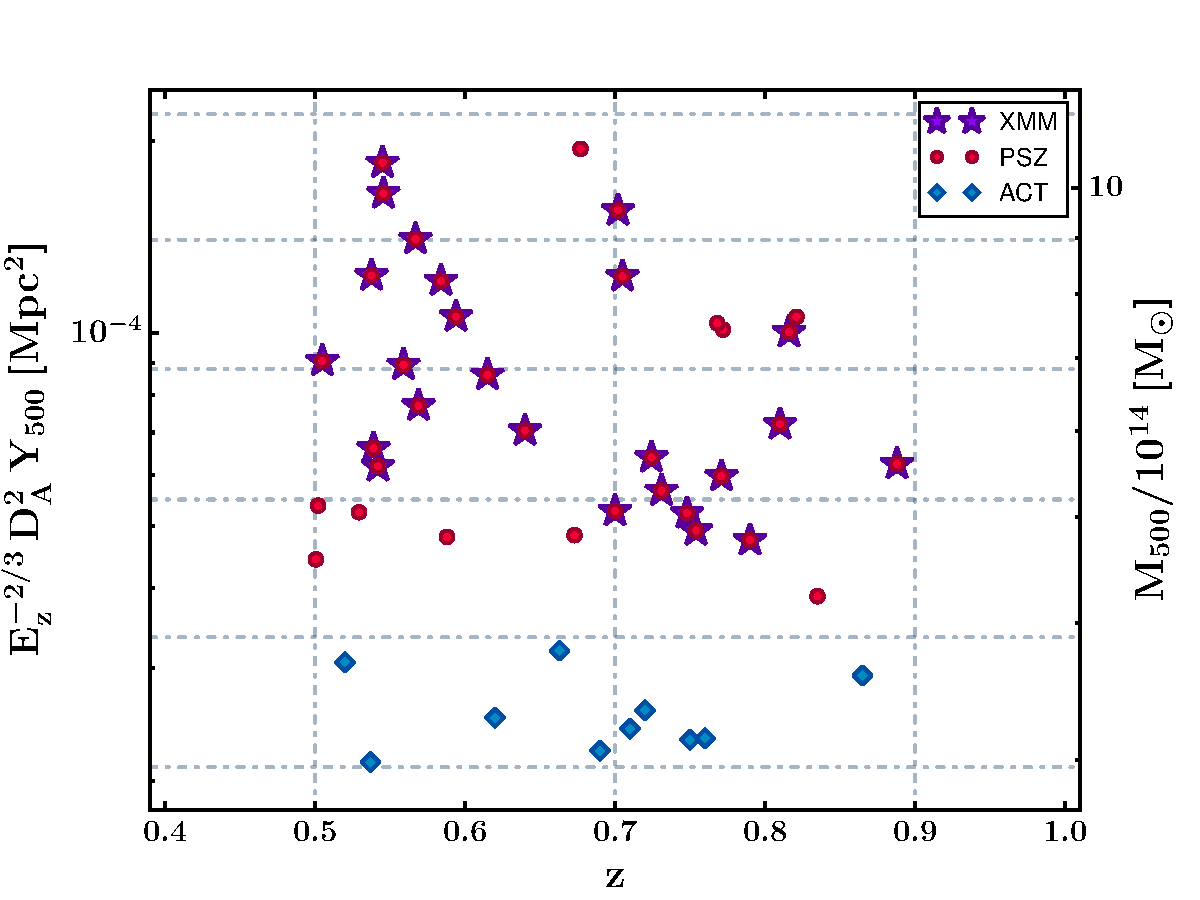
\includegraphics[width=0.44\textwidth, clip=true, trim=0cm -0.7cm 0cm 0cm]{Figures/NIKA2-SZ/LPSZ_M_z_grid.pdf}
  \caption{Left: Map of the kinetic SZ effect toward \mbox{MACS~J0717.5+3745} using NIKA pathfinder data, as discussed in Adam et al. (2017)$^{31}$. Right: NIKA2 Guaranteed-time cosmology program sample of galaxy clusters}
  \label{fig:LP-SZ}
\end{figure}
%
L'échantillon se distribue dans
deux intervalles de redshifts, les redshifts intermédiaires dans la
gamme 0.5 à 0.7 et les hauts redshifts entre 0.7 et 0.9. Il se découpe
en cinq intervalles en masse, définis à partir de la quantité
$E_{z}^{-2/3} D_{\rm{A}}^2 Y_{500}$ fortement corrélée à la masse. Cette
quantité dépend de l'observable tSZ intégré $Y_{500}$ et du modèle
cosmologique à travers $E_{z} = H(z)/H_0$ et $D_{\rm{A}}$, la distance
angulaire. Nous avons sélectionné cinq amas cibles dans chacun des
intervalles en redshift et en masse en utilisant des critères assurant
la représentativité de l'échantillon. Cette propriété est fondamentale
pour fournir des mesures des relations d'échelle et des profils
thermodynamiques applicables à l'ensemble des amas et donc utiles pour
les analyses cosmologiques. Comme discuté à la Sect.~\ref{se:cosmo_sz}, une
sélection basée sur le signal tSZ capture presque tous les amas
au-dessus d'un seuil en masse, et définit bien un échantillon
représentatif. Ainsi, les amas du LP-SZ sélectionnés sont ceux
appartenant à un catalogue d'amas détectés via le tSZ, dont le
redshift est dans la gamme 0.5-0.9 et qui sont observables depuis le
télescope de 30-m de l'IRAM. Pour ce dernier critère, nous retenons
les amas dont la déclinaison est $\delta > -11^{\circ}$, comme figuré
par le cercle pointillé sur le panneau de gauche de la
Fig.~\ref{fig:LP-SZ}. Les quatre intervalles de plus hautes masses sont
peuplés par des amas sélectionnés dans le premier catalogue de
\emph{Planck}~\citep[le seul disponible au moment de la définition de
l'échantillon][]{Planck2013_SZcat}, tandis que les amas de
l'intervalle de basse masse sont issus du catalogue
ACT~\citep{Hasselfield2013_ACT_SZ}.

Par ailleurs, les observations tSZ avec NIKA2 seront complétées par
des suivis avec d'autres sondes. En particulier, la complémentarité
avec les observations dans le domaine X avec le satellite
\emph{XMM-Newton} est l'une des forces du LP-SZ. Les amas du LP-SZ
également observés par \emph{XMM-Newton} sont repérés avec une étoile
dans le panneau de droite de la Fig.~\ref{fig:LP-SZ}. Des demandes de
suivi avec \emph{XMM-Newton}, portées par l'équipe du LP-SZ, sont en
cours.   

\subsection{Objectifs et livrables}

L'objectif premier du LP-SZ est de fournir à la communauté des cartes
à haute résolution angulaire de l'effet tSZ, ainsi que les profils de
pression reconstruits, pour un échantillon représentatif d'amas de
galaxies. Ces données permettront une étude approfondie des propriétés
des amas de galaxie jusqu'à haut redshift et de leur évolution
cosmologique. De même qu'un profil de pression universel a été mesuré
avec \emph{REXCESS}, un échantillon représentatif de 33 amas observés
avec \emph{XMM-Newton} dans l'univers proche
($z<0.2$)~\citep{Arnaud2010}, l'échantillon du LP-SZ permettra de
tester la régularité du profil de pression jusqu'à $z=0.9$ à partir
d'une observable sondant directement la pression. Aussi, l'impact des
sous-structures et de la morphologie des amas sur l'observable $Y_{500}$
pourra être quantifié. Des indicateurs de l'état dynamique des amas
pourront être défini à partir des observations tSZ. Ainsi, le LP-SZ
permettra de caractériser l'impact des déviations au
comportement auto-similaire sur le biais et la dispersion intrinsèque
de la relation d'échelle et du profil de pression moyen, et leur
évolution en redshift. Ces résultats attendus auront d'importantes retombées
pour la cosmologie avec les amas de galaxies.

Les objectifs scientifiques peuvent encore être étendus en exploitant
la complémentarité avec d'autres sondes des amas, et en premier lieu,
les observations dans le domaine des X. Gràce à l'expérience NIKA2, le
milieu intra-amas sera cartographié via l'effet tSZ avec le même
niveau de précision qu'en X, tant en résolution angulaire qu'en
sensibilité. Ainsi, une étude conjointe des données tSZ de NIKA2 et
des données X de \emph{XMM-Newton} permettra une caratérisation
complète des propriétés thermodynamiques des amas. Aux profils de
pression électronique $P_e(r)$ reconstruits dans les données tSZ, nous
adjoindrons les profils de densités $n_e(r)$ estimés dans les données
X. Une telle étude multi-sonde nous permettra de mesurer le profil de
température $k_{\rm{B}} T_e(r) = P_e(r)/n_e(r)$, sans avoir recourt
aux mesures spectroscopiques en X, ainsi que le profil
d'entropie $K(r) = P_e(r)/n_e(r)^{5/3}$, un bon indicateur de l'état
dynamique des amas. Ensuite, sous l'hypothèse de l'équilibre
hydrostatique, nous reconstruirons le profil de masse hydrostatique
des amas $M_{\rm{HE}} (r) \propto r^2/n_e(r) dP_e(r)/dr$.  
%\begin{equation}
%  M_{\rm{HE}} (r) = - \frac{r^2}{\mu_{\rm{gaz}}m_pn_e(r)}
%\end{equation}
L'étude statistique de ces profils thermodynamiques sera essentielle
pour caractériser les propriétés physique des amas, leur évolution en
redshift et la relation entre l'observable tSZ et la masse des amas.  


\subsection{L'équipe}
Le LP-SZ mobilise une équipe d'une vingtaine de chercheurs fortement
impliqués, comprennant des experts de l'effet SZ, qui ont joué un rôle
majeurs dans l'analyse des amas de galaxies dans \emph{Planck} et ont
mené des études tSZ à partir des observations de NIKA, des experts de
renommée mondiale des amas de galaxies observés en X, des experts de
simulations hydrodynamiques et des experts d'autres sondes d'amas
(observations optiques et radio). Par ailleurs, plusieurs membres ont
une connaissance très fine de l'instrument NIKA2. En tant que co-PI,
je coordonne les activités conjointement avec le PI.



%----------------------------------------------------------------------------------------
%
%
%
%
%
%                 ETUDES PILOTES ET Premiers resultats 
%
%
%
%----------------------------------------------------------------------------------------
\section{Les études pilotes et les premiers résultats}
\label{se:NIKANIKA2_SZ}

\subsection{\'Etudes pilotes avec le prototype NIKA}
\label{se:NIKA_SZ}

Pour démontrer les capacités de NIKA2 pour la cartographie
haute-résolution de l'effet tSZ, valider et optimiser la définition
des objectifs scientifiques et préparer l'analyse, nous avons d'abord
réalisé une séries d'études ``pilotes'' avec l'instrument précurseur
NIKA. Ainsi, la première détection de l'effet tSZ jamais obtenue avec
la technologie KID a été réalisée avec les observations de NIKA vers
l'amas RX\,J1347.5-1145, un amas massif à redshift intermédiaire
($z = 0.45$)~\citep{Adam2014}. Ensuite, pour préparer l'analyse tSZ de
NIKA2, des méthodes novatrices ont été développées et testées sur les
observations de NIKA. Par exemple, nous avons développé une analyse
multi-sonde combinant données tSZ et données X qui a été testée sur un
amas à haut redshift ($z = 0.89$), CL\,J1226.9+3332, observé avec NIKA
et appartenant au catalogue de données publiques de
\emph{CHANDRA}~\citep{Adam2015}. Aussi, en ciblant un amas bien régulier,
MACS\,J1423.9+2404, nous avons caractérisé l'impact des sources
ponctuelles radio et infrarouge et proposé une méthode pour les
traiter dans le cadre d'une analyse tSZ~\citep{Adam2016}. Une méthode
non-paramétrique pour reconstruire le profile de pression à partir de
la carte tSZ a été proposée et validée avec les données de NIKA et
\emph{Planck} seules~\citep{Ruppin2017} et en considérant aussi les
données de MUSTANG et BOLOCAM~\citep{Romero2018}. Nous avons exploré
la présence de sous-structures dans le milieu intra-amas, signant
l'état dynamique de l'amas, en testant plusieurs outils de détection
dans les cartes tSZ de NIKA~\citep{Adam2018_sub}. Cette étude, qui a
accompagnée la livraison des données tSZ de NIKA à la communauté,
constitue une validation de la possibilité pour NIKA2 de caractériser
l'impact de l'état dynamique des amas sur le profil de pression moyen
et la relation masse-observable tSZ.

%
\begin{figure}
  \centering
  \includegraphics[width=0.40\textwidth]{Figures/NIKA2-SZ/MACSJ0717_T_map.pdf}
  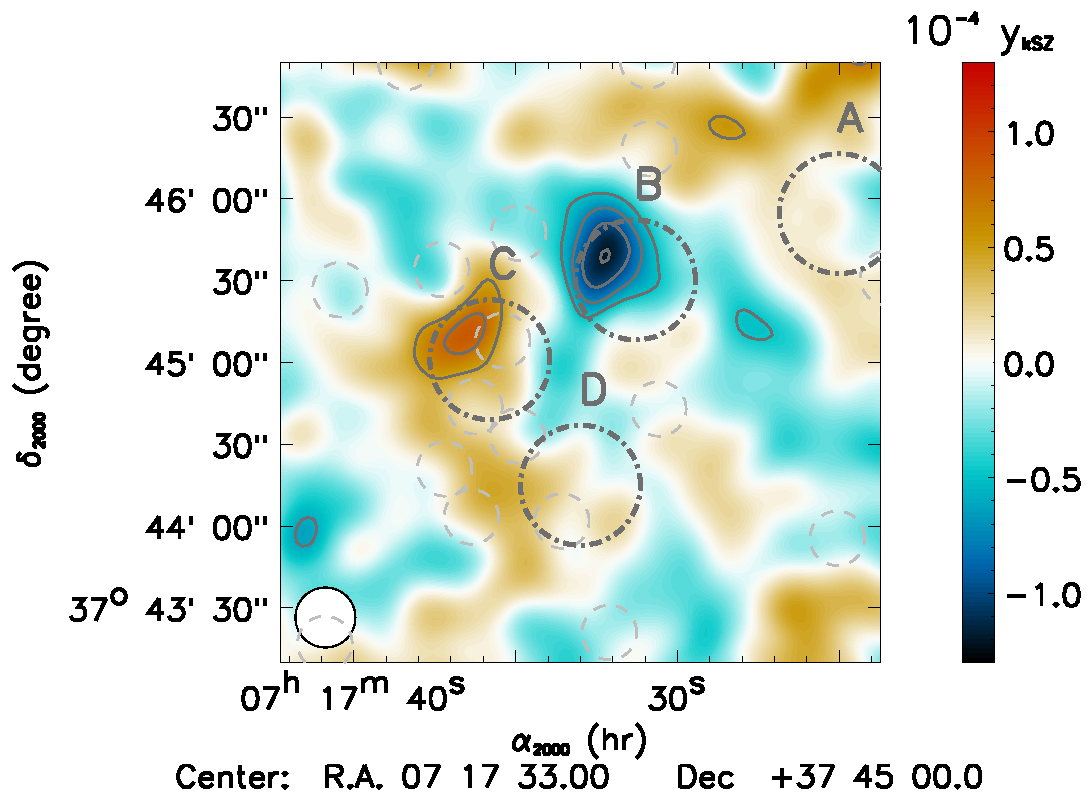
\includegraphics[width=0.56\textwidth]{Figures/NIKA2-SZ/MACSJ0717_kSZ_map.pdf}
  \caption{Map of the kinetic SZ effect toward \mbox{MACS~J0717.5+3745} using NIKA pathfinder data, as discussed in Adam et al. (2017)$^{31}$.}
  \label{fig:nikanika2}
\end{figure}
%
Ces études pilotes nous ont aussi permis d'obtenir des résultats
remarquables, allant au-délà de ce qui étaient initialement espéré, et
marquant une percée vers des études novatrices. En particulier,
la première carte de la température du milieu intra-amas reconstruite
avec l'effet SZ est décrite dans~\citet{Adam2017} et la première carte
de l'effet SZ cinétique (kSZ) mesuré dans un amas a été obtenue 
dans~\citet{Adam2017kSZ}. Ici nous présentons brièvement ces deux
résultats.

La température du milieu intra-amas est une observable fondamentale pour
caractériser les amas de galaxies, en particulier pour déterminer leur
masse hydrostatique. Cette température est généralement obtenue par
mesures spectrométriques dans le domaine X. Cette méthode a plusieurs
limitations bien connues. L'émission X étant proportionnelle au carré
de la densité du milieu intra-amas, les mesures en X sélectionnent
préférentiellement les zones denses et froides des amas. Ensuite, les
mesures de température via les expériences X actuels, tels
\emph{XMM-Newton} et \emph{Chandra}, sont affectées par l'incertitude
sur la calibration absolue en énergie, qui est de l'ordre de
$15\%$. Enfin, une mesure précise de la température par spectroscopie
X requiert de longs temps d'observation, qui peuvent même devenir
prohibitifs pour les amas distants. Une autre méthode pour obtenir la
température du milieu intra-amas consiste à la reconstruire à partir
de la pression électronique mesurée via l'effet tSZ et de la densité
mesurée par photométrie X, par exemple. En utilisant cette méthode,
\citet{Adam2017} a construit la première carte de la température d'un
amas, MACS\,J0717.5+3745, en combinant les observations SZ
haute-résolution de NIKA et les données photométriques de
\emph{XMM-Newton}. Cette carte, présentée dans le panneau de gauche de
la figure~\ref{fig:nikanika2}, met en évidence un fort gradient de
température dans la région de collision entre les deux principaux
sous-amas. Elle est compatible avec les cartes de température dérivées
des données spectroscopiques de \emph{XMM-Newton} et \emph{Chandra},
tout en étant moins bruitées et obtenue avec un temps d'observation
trois fois moindre.


L'effet kSZ est dù au mouvement d'ensemble du milieu intra-amas, il
dépend à la fois de la densité du gaz et de sa vitesse propre par
rapport au référentiel du CMB et, contrairement au tSZ, ne crée pas de
distortion spectrale (voir discussion Sect.~\ref{se:cosmo_sz}). Par
conséquent, sa signature en fréquence diffère de celle du tSZ. En
combinant des cartes dans différent canaux de fréquence du domaine
millimétrique, les deux composantes peuvent être séparées, et une
carte reconstruite pour chacune d'entre elle. En pratique, une telle
étude requiert une expérience qui allie une haute sensibilité, afin de
détecter cet effet sous-dominant, et une grande résolution angulaire
afin de séparer spatialement le kSZ du CMB. Le panneau de droite de la
figure~\ref{fig:nikanika2} présente la première carte résolue
du kSZ, obtenue par~\citet{Adam2017kSZ} en combinant les
observations à 150 et 260\,GHz effectuées avec NIKA vers l'amas
MACS\,J0717.5+3745. Cet amas bien connu, déjà choisi comme
cible pour cartographier la température, est un système complexe, très
perturbé, composé de plusieurs sous-amas en interaction, avec des
vitesses relatives extrêmes (de l'ordre de 1000\,km/s). Ces sous-amas
sont entourés en gris sur la figure~\ref{fig:nikanika2}, deux d'entre
eux tombent l'un vers l'autres et induisent un effet kSZ de signe
opposé. En combinant les cartes de NIKA avec une mesure de la
température du gaz issue des données spectroscopiques de
\emph{XMM-Newton}, les cartes de densité et de vitesse du gaz ont été
reconstruites en supposant un modèle de gaz. Ainsi a été obtenue la
première carte résolue de la vitesse au sein du milieu intra-amas
mesurée via l'effet kSZ.

Ces résultats nous donnent une grande confiance dans notre capacité à
réaliser les objectifs scientifiques que nous nous somme fixés dans le
cadre du LP-SZ et au-delà, de l'utilité pour la cosmologie des
observations CMB à très haute résolution.

\subsection{Premiers résultats de NIKA2}

Les observations des amas de galaxies du LP-SZ ont d'ores et déjà
commencées. La première observation d'un amas a été
effectuée dès la phase de vérification scientifique de NIKA2 en avril
2017 (voir l'historique à la Sect.~\ref{}), puis les observations se
sont poursuivies depuis l'ouverture de NIKA2 à la communauté en
octobre 2017, de sorte que 19 amas du LP-SZ ont été observés pour un
temps d'observation total d'environ 80 heures.


Pour la vérification scientifique, nous avons sélectionné un amas du
LP-SZ avec un fort signal tSZ attendu et pour lequel nous disposions
aussi de données X à haute précision. Ainsi, le premier amas observé
du LP-SZ est PSZ2\,G0144.83+25.11, un amas bien connu, massif
($\rm{M} = 7.8\,10^{14}\,\rm{M}_{cdot}$), à redshift intermédiaire
($z=0.58$) et observé également par \emph{XMM-Newton}. Les données
NIKA2 consistent en 11 heures d'intégration sur la source, soit cinq
fois plus que le temps demandé dans le LP-SZ pour cet amas, mais dans
des conditions de forte attenuation atmosphérique (opacité de 0.3 à
150\,GHz). Après soustraction des sources ponctuelles par une méthode
adaptée de celle de~\citet{Adam2016}, nous avons
obtenu la première carte du paramètre de Compton vers un amas de
galaxie avec NIKA2. Cette carte, décrite dans~\citet{Ruppin2018}, est
présentée dans le panneau de gauche de la figure~\ref{fig:nika2-sz}.
%
\begin{figure}
  \centering
  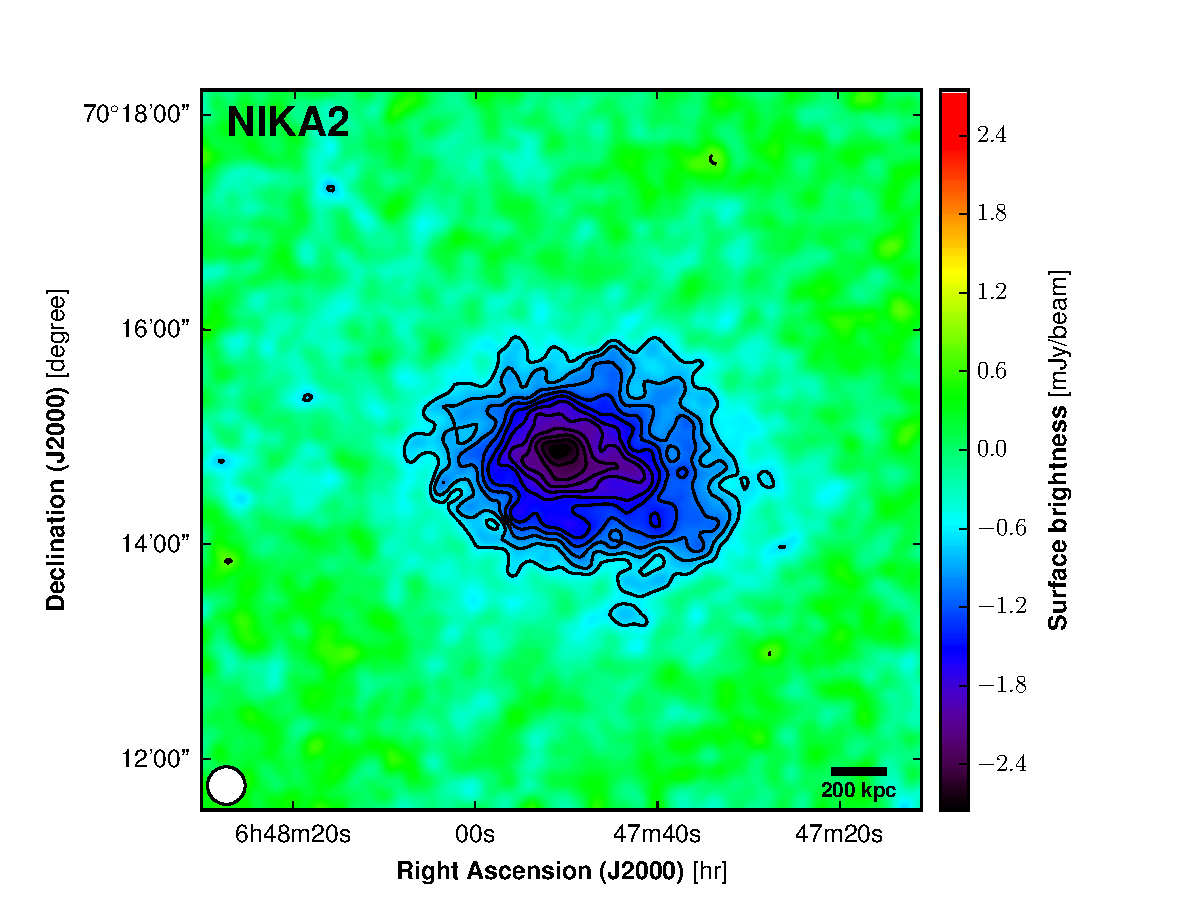
\includegraphics[width=0.49\textwidth]{Figures/NIKA2-SZ/Paper_NIKA2_Data.pdf}
  \includegraphics[width=0.44\textwidth]{Figures/NIKA2-SZ/Fig_PSZ2_G144_Scaling_relation.pdf}
  \caption{First SZ results with NIKA2. Left: The NIKA2 SZ map toward the galaxy cluster PSZ2-G0144.83+25.11. The high-resolution (20~arcsec) high-accuracy ($13.5\sigma $ measurement at peak) map covers the cluster from the core to the outskirts and reveals its morphology. An excess SZ signal is observed in the South-West region, indicating an overpressure within the intracluster medium (ICM). Right: Illustration of the impact of the ICM dynamics on the inner scatter of the SZ mass-observable relation. NIKA2 $Y_{500}$ estimates from the analysis with and without masking the over-pressure of PSZ2-G0144.83+25.11 are shown as a function of $M_{500}$, along with the cluster sample and the $Y_{500}-M_{500}$ scaling relation used in \emph{Planck} SZ-selected cluster count based cosmology analysis$^{13}$. These figures are extracted from Ruppin {\it et al.} (2018)$^{34}$. }
  \label{fig:nika2-sz}
\end{figure}
%
Nous avons identifié une zone de sur-pression thermique dans l'extension sud-ouest
de l'amas, qui est repérée par la zone grisée sur la
figure~\ref{fig:nika2-sz}. Pour cet amas, en plus des cartes tSZ de
NIKA2 et \emph{Planck}, nous disposons de la carte tSZ de MUSTANG, dont
la résolution angulaire est de 9'' et le champ de vue de
42''~\citep{Young2015}, ainsi que de celle de BOLOCAM, sur un champ de
vue de 8' pour une résolution angulaire de l'ordre de
1'~\citep{Sayers2013}. Tout d'abord, en combinant l'ensemble des
données tSZ, nous avons obtenue une mesure non-paramétrique du profil
de pression depuis le coeur de l'amas ($\sim 0.02\rm{R}_{500}$)
jusqu'à sa périphérie ($\sim 3\rm{R}_{500}$) en utilisant la méthode
développée dans~\citet{Ruppin2017}. Ensuite, nous avons exploré
l'impact de la sur-pression en comparant les profils de pression
reconstruits soit dans les cartes tSZ de NIKA2 et \emph{Planck}
complètes, soit en masquant la sur-pression. Nous observons une
différence significative entre les deux profils résultants. Le profil
déprojetté sur les cartes masquées est en accord avec le profil de
pression universel décrit dans~\citet{Arnaud2010}, mais dévie
significativement du profil obtenu dasn les cartes non-masquées, ce
dernier étant en accord avec le profil publié dans~\citet{Young2015} à
partir des cartes tSZ complètes de MUSTANG et BOLOCAM. 
Pour aller plus loin, nous avons réalisée une analyse conjointe des
données tSZ de NIKA2 et \emph{Planck} et des données X de
\emph{XMM-Newton}, en utilisant une méthode adaptée
de~\citet{Adam2015}, pour dériver les profils thermodynamiques de
l'amas sous l'hypothèse d'équilibre hydrostatique. Nous trouvons que
le paramètre de Compton intégré jusqu'à $R_{500}$, $\rm{Y}_{500}$ et
la masse hydrostatique $\rm{M}_{500}$ résultant des analyses
hydrostatiques effectuées avec ou sans le masque de la zone de
sur-pression diffèrent significativement. Ces valeurs sont reportées
dans le panneau de droite de la figure~\ref{fig:nika2-sz}, et
superposées aux quantités intégrées pour l'échantillon d'amas de
\emph{Planck} qui a servi à calibrer la relation d'échelle utilisée
pour les résultats
cosmologiques~\citet{Planck_2014_SZ_Cosmo,Planck_2016_SZ_cosmo}. Cette
étude est une indication de l'impact de l'état thermodynamique des
amas sur la dispersion intrinsèque de la relation
masse-observable. Elle illustre bien l'utilité de NIKA2, combinée avec
des données X, pour caractériser la relation d'échelle.   






%----------------------------------------------------------------------------------------
%
%
%
%
%
%                 Prospectives ? 
%
%
%
%----------------------------------------------------------------------------------------
\section{Développement de l'analyse, implication pour la cosmologie et perspectives}

\subsection{Préparation de l'analyse cosmologique}

\`A court terme, l'équipe du LP-SZ s'attachera à préparer l'analyse, la
publication et la livraison à la communauté scientifique des données
et résultats d'intérêt cosmologique.

\subsubsection{Vers une méthode standard d'analyse}
La première étape consistera en 1)
l'amélioration et 2) la standardisation des outils d'analyse. Les
améliorations viseront en priorité le traitement des sources
ponctuelles, qui constituent le contaminant majeur des cartes tSZ de
NIKA2. Une telle étude, centrée sur l'optimisation du traitement des
sources ponctuelles infrarouge pour les amas les moins brillants de
l'échantillon du LP-SZ, est déjà en cours~\citep{Keruzore2020}.

Un deuxième champ d'amélioration crucial concerne la reconstruction
des grandes échelles angulaires. En effet, tandis que les observations en X
révèlent bien les zones centrales (denses et froides) de l'amas, les
observations tSZ permettent une cartographie s'étendant sur de grandes
distances jusque dans la périphérie de l'amas. Pour exploiter au mieux
cette caractéristique et bénéficier du grand champ de vue de NIKA2, il
nous faut développer des outils d'analyse qui préservent les grandes
échelles angulaires. Or nos méthodes actuelles sont efficaces pour
soustraire le bruit corrélé issu majoritairement de l'émission
atmosphérique, au prix d'un filtrage spatial~\citep[voir par
  exemple][]{Ruppin2018}. Des pistes de développement de nouvelles
méthodes sont actuellement explorées.

Quant à la standardisation des outils d'analyse, elle est nécessaire
afin de ne pas briser la représentativité de l'échantillon d'amas du
LP-SZ en introduisant des biais méthodologiques. Il nous faudra
développer des outils robustes, applicables pour toutes les
morphologies d'amas et pour toutes la gamme de signal tSZ sondé. Ces
méthodes seront testées et optimisées sur des simulations.

\subsubsection{Validation et études prospectives}

La validation des outils d'analyse sur simulation est un volet
important du LP-SZ. Nous déployons à la fois des simulations simples,
utilisant un profil de pression universel pour synthétiser un signal
tSZ, permettant une analyse Monte-Carlo, et à la fois des simulations
réalistes. Ces dernières sont basées sur la simulation hydrodynamique
\emph{Marenostrum MUltidark SImulations of galaxy
  Clusters}~\citep[MUSIC][]{Sembolini2013}. Ainsi, un échantillon
d'amas synthétiques a été extrait de la simulation MUSIC de façon à
obtenir un échantillon similaire à celui du LP-SZ. Cet échantillon
``jumeau", qui présente le même peuplement dans le plan
masse-redshift, est décrit dans~\citet{Ruppin2019a}. Il a été utilisé
pour tester nos outils de reconstruction du profil de pression dans le
milieu intra-amas. Pour cela, des observations réalistes des amas
synthétiques par NIKA2 et \emph{Planck} ont été simulées, et les
profils de pression estimés sur ces simulations. La comparaison entre
les profils de pression moyens reconstruits et simulés nous permet de
valider les méthodes de reconstruction. \citet{Ruppin2019a} ont montré
que le profil de pression moyen était bien reconstruit, avec une
précision de l'ordre du pourcent, quelque soit l'état dynamique de
l'amas. En plus du test des méthodes d'analyse, cette étude a mis en
évidence l'impact sur le profil de pression moyen de l'état dynamique
des amas. En effet, la dispersion intrinsèque du profil de pression
moyen est sensiblement plus grande pour les amas perturbés, présentant
des sous-structures, que pour les amas réguliers, à l'équilibre
hydrostatique. Bien que la forme et la dispersion du profil moyen
dépendent de l'échantillon synthètique, cette étude prospective est
bien représentative des résultats qui pourront être obtenus dans le
cadre du LP-SZ. D'autres études prospectives pourront être menées en
exploitant les simulations MUSIC, incluant l'optimisation de critères
dichotomiques de l'état thermodynamique des amas
(réguliers/perturbés) ou la caractérisation de l'impact d'une déviation
à l'auto-similarité sur le profil de pression moyen et la relation
masse-observable.

\subsubsection{Préparation de la livraison des données et des résultats}

Nous nous attacherons à préparer la livraison des données à la
communauté, et la publication des résultats d'intérêt cosmologique,
qui devront avoir lieu entre 2022 et 2025. En plus des cartes tSZ à hautes
résolution angulaire de NIKA2, nous publierons notre caractérisation
du profil de pression universel et de la relation masse-observable,
et dériverons les implications pour la cosmologie. 
%
\begin{figure}
  \centering
  \includegraphics[width=0.49\textwidth]{Figures/NIKA2-SZ/NIKA2cosmo_echantillon_calibration.pdf}
  \includegraphics[width=0.49\textwidth]{Figures/NIKA2-SZ/NIKA2cosmo_param.pdf}
  \caption{Left: Distribution of the 62 Planck clusters used to
    estimate the mean normalized pressure profile at low redshift
    (purple) in the mass-redshift plane. The NIKA2 and REXCESS samples
    are also shown in orange and green respectively.
    The different shades of blue give the expected cluster abundance,
i.e. the cluster number per unit of mass and redshift. Right:
Constraints obtained on the $\sigma_8$ and $\Omega_m$ cosmological
parameters using the Pm profile (grey) and the Pm profile scaled down
by 15\% (green) for a possible future hydrostatic bias prior of $b = 0.20
\pm 0.01$. The constraints obtained from the joint analysis of the CMB
primary anisotropies and BAO data are also shown in purple. Figures
from~\citet{Ruppin2019b}}
  \label{fig:nika2cosmo}
\end{figure}
%
Le LP-SZ résultera en une amélioration de la calibration de la masse des
amas de galaxies et de leur contenu thermodynamique par rapport à
notre connaissance actuelle. Ce potentiel d'amélioration est illustré
dans le panneau de gauche de la
figure~\ref{fig:nika2cosmo}. L'échantillon d'amas du LP-SZ est comparé
aux échantillons d'amas qui fondent actuellement la calibration des
amas de galaxies dans les analyses cosmologiques de
\emph{Planck}~\citep{Planck_2014_SZ_Cosmo,
  Planck_2014_ymap, Planck_2016_SZ_cosmo, Planck2016_ymap,
  Salvati2018}. Dans le plan mass-redshift, sont figurés l'échantillon
de 45 amas du LP-SZ, qui couvre l'intervalle $0.5 \le z \le 0.9$,
l'échantillon de 62 amas de \emph{Planck} à $z<0.5$ sur lequel est
calibré le profil de pression moyen, et l'échantillon de 31 amas de
REXCESS~\citep{Pratt2009} qui a servi à calibrer la relation
masse-observable et le profil de pression universel via les
observations en X, comme décrit dans \citet{Arnaud2010}. En sondant un
échantillon d'amas distants,
le LP-SZ permettra de contraindre l'évolution en redshift des
propriétés des amas et fournira des mesures de la relation
masse-observable et du profil de pression moyen bien adaptées aux
relevé d'amas cosmologiques. En améliorant la calibration des amas de
galaxies, qui constitue la limitation principale des études
cosmologiques, nous améliorerons la robustesse et la précision des
contraintes cosmologiques dérivées des amas de galaxies.

Dans des études prospectives, nous pouvons déjà prédire l'impact des
résultats du LP-SZ sur la cosmologie. Par exemple, \citet{Ruppin2019b}
ont étudié l'impact du profil de pression moyen sur les contraintes
cosmologiques dérivées du spectre de puissance angulaire de l'effet
tSZ de \emph{Planck}. Dans le cadre du modèle $\Lambda$CDM standard,
nous avons trouvé des différences signicatives sur les paramètres
cosmologiques estimés en fonction du  profil de pression moyen supposé
dans l'analyse cosmologique. Dans le panneau droit de la
figure~\ref{fig:nika2cosmo}, nous traçons les contours à 68 et 95\% de
niveau de confiance de la distribution de paramètres dans le plan
$\sigma_8$, $\Omega_{\rm{m}}$ pour trois analyses cosmologiques :
une analyse conjointe du CMB de
\emph{Planck}~\citep{Planck_2018_cosmo} et des oscillations
acoustiques des baryons (BAO) de BOSS~\citet{Anderson2014}, l'analyse
du $C_\ell^{\rm{tSZ}}$ de \emph{Planck} en supposant le même profil de
pression moyen que celui utilisé dans \citet{Planck2016_ymap} et la
même analyse réitérée avec un profil de pression moyen d'une amplitude
15\% inférieure. Nous concluons qu'une diminution de 15\% de
l'amplitude du profil de pression moyen suffit pour pour faire
coïncider les modèles cosmologiques favorisés par le CMB primaire et
par les amas de galaxies sans avoir recours à des valeurs extrêmes du
biais hydrostatique. L'apport du LP-SZ sur la mesure du profil de
pression moyen et son évolution en redshift sera donc précieux pour
contraindre la cosmologie avec les amas de galaxies. 

D'autres études prospectives pourront être menées pour anticiper la
livraison des résultats du LP-SZ. Par exemple, une évolution de la
forme ou la dispersion intrinsèque de la relation masse-observable
pourrait biaiser l'estimation de la fonction de sélection de
l'échantillon cosmologique dans le cadre d'une analyse fondée
sur le comptage des amas, et aurait ainsi un impact important sur le
modèle cosmologique estimé. Ou encore, une étude similaire à
celle menée dans~\citet{Ruppin2019b} pourrait être conduite dans le
cadre d'un modèle cosmologique étendu en utilisant les outils
développés dans~\citet{Bolliet2018, Bolliet2019} pour étudier l'impact
de la calibration des amas de galaxies sur les contraintes de
l'énergie noire ou la masse des neutrinos.\\

Le travail décrit dans cette section, et qui aboutira à la
publication des résultats du LP-SZ pourrait faire l'objet d'une thèse
de doctorat commençant au début de la décennie 2020. 

\subsection{\'Etudes multi-sondes complémentaires}

Au delà de l'analyse principale centrée sur la combinaison des données
X et tSZ, décrite à la section précédente, des analyses multi-sondes
complémentaires pourraient encore enrichir les résultats du LP-SZ. 

\subsubsection{Relation entre milieu intra-amas et galaxies avec les
  données optiques}

Des données de haute qualité en imagerie et en spectroscopie optique
et proche infrarouge, utilisées en combinaison avec le tSZ et le X,
conduiraient à plusieurs développements importants. Nous disposerions
alors à la fois des mesures de la richesse, c'est-à-dire le nombre de
galaxies membres, et des mesures de leur dispersion de vitesse, nous
fournissant chacunes une estimation supplémentaire de la masse des
amas, fondées sur des hypothèses différentes de la masse hydrostatique
tSZ-X et non affectées par les même effets systématiques. De telles
études combinées nous permettraient d'explorer les correlations entre
la richesse, la masse dynamique, calculée à partir de la dispersion de
vitesses, et la masse hydrostatique et plus généralement la relation
entre les propriétés des galaxies au sein des amas et le milieu
intra-amas.

Pour ce programme, nous avons envisagé d'effectuer un suivi des amas
du LP-SZ avec les imageurs et spectromètres installés au \emph{Gran
  Telescopio Canarias} (GTC), le télescope de 10.4 mètres de
l'\emph{Instituto de Astrofísica de Canarias} (IAC), situé sur l'île
de La Palma. Ce télescope est bien adapté pour le suivi optique des
amas \emph{Planck} distants et visibles depuis l'hémisphère
nord. Un tel suivi est actuellement en cours dasn le cadre des grands
programmes d'observation optique visant à la validation et la
caractérisation des catalogues d'amas de
\emph{Planck}~\citep{Barrena2018,Streblyanska2019,Aguado-Barahona2019}.
Pour le suivi des amas du LP-SZ, des observations plus profondes
seront nécéssaires afin de caractériser la structure interne des
amas. Quelques heures d'observation par amas avec la caméra OSIRIS du
GTC permettraient d'effectuer à la fois une photométrie dans les
filtres \emph{GRIZ} et une spectroscopie multi-objets avec un rapport
signal-sur-bruit suffisant pour caractériser la distribution des
galaxies membres dans l'espace des phases. Des études multi-sondes
combinant les données tSZ, X et optique donneraient de précieuses
indications sur l'interaction des populations de galaxies avec le
milieu inter-amas. Ensuite, un suivi en spectro-imagerie optique de
l'échantillon du LP-SZ permettrait d'une part de contraindre la
relation entre masse dynamique et la masse hydrostatique et son
évolution en redshift, et d'autre part de mieux comprendre la
formation et l'évolution des populations de galaxies dans les amas.
Une telle étude, complémentaire aux objectifs c\oe ur du LP-SZ,
auraient d'importantes implications pour la cosmologie avec les amas
de galaxies, en particulier dans le cadre de futurs relevés optiques
(Euclid, LSST). 


\subsubsection{Contraindre le biais hydrostatique et la pression
  non-thermique avec l'effet de lentille}

Les effets de lentille fort et faible sur les galaxies d'arrière-plan
dépendent du potentiel gravitationnel de l'amas intégré le long de la
ligne de visée, et permettent ainsi une reconstruction de la masse
totale de l'amas. Les effets systématiques qui impactent cette mesure
sont de nature instrumentale (incertitude sur la PSF), méthodologique
(calibration du cisaillement, contamination par des galaxies
d'avant-plan) ou géométrique (alignement, tri-axialité, décentrage),
mais ne dépendent pas de l'état thermodynamique de l'amas. Ainsi, des
analyses conjointes du tSZ, des X et des lentilles
permettent à la fois de mieux contraindre la masse des amas, et à la
fois de tester les hypothèses qui fondent l'estimation de la masse à
partir de chacune de ces observables. Comme mentionné dans la
Sect.~\ref{se:cosmo_tensions}, de telles analyses, utilisant les
programmes de reconstrution de l'effet de lentille récents (Weighting
the Giants, CCCP, LoCuSS), ont permis de mesurer le biais
hydrostatique~\citep[voir][pour une compilation des
  résultats]{Salvati2018, Osato2019}. Autre exemple pris dans la littérature
récente, \citet{Siegel2018} ont combiné le tSZ mesuré par BOLOCAM, les
données X de \emph{Chandra} et les effets de lentilles mesurés avec le
\emph{Hubble Space Telescope} (HST) et \emph{Subaru Suprime-Cam}. En
comparant le profil de pression thermique estimé dans les données
tSZ-X et le profil de pression totale nécessaire pour empêcher
l'effondrement gravitationel, ils ont déduit une mesure de la pression
non-thermique, induite par la turbulence ou les écoulements au sein du
milieu intra-amas. De la même façon, les données tSZ-X du LP-SZ,
combinées aux mesures existantes de l'effet de lentille, nous
permettront de mesurer le biais hydrostatique et la fraction de pression
non-thermique et de contraindre leur évolution en redshift.  

\subsubsection{Mesurer la pression électronique jusqu'au c\oe eur des
  amas : synergie avec NOEMA}

NIKA2 cartographiera les amas de galaxies avec une résolution angulaire
et une sensibilité comparable à celles de \emph{XMM-Newton},
permettant une exploitation optimale de la complémentarité des données
X et tSZ au sein du LP-SZ. Ce programme bénéficierait d'observations à
encore plus haute résolution angulaire pour déceler l'impact des
processus astrophysiques dans le milieu intra-amas, en particulier au
c\oe ur des amas. Pour cela, l'interférométrie millimétrique est
parfaitement adaptée puisqu'elle permet une cartographie très haute
résolution des amas distants via l'effet tSZ. Dans l'hémisphère sud,
l'interféromètre millimétrique phare est ALMA. La complémentarité des
observations tSZ à résolution angulaire de quelques secondes d'arc à
quelques minutes d'arc a été exploitée pour une mesure complète du
profil de pression d'un amas en combinant les données
interférométriques d'ALMA avec les données des imageurs BOLOCAM et
\emph{Planck}~\citep{DiMascolo2019}. Dans l'hémisphère nord, le plus
grand interféromètre millimétrique actuellement en opération est le
\emph{NOrthern Extended Millimeter Array} (NOEMA) de l'IRAM.

NOEMA\footnote{Site web :
  \url{https://www.iram-institute.org/EN/content-page-56-7-56-0-0-0.html}}
est un réseau de 10 antennes de 15 mètres de diamètres, installé
au Plateau de Bure. Il observe dans trois bandes
de fréquence centrées à 90, 150 et 230 GHz avec une résolution
angulaire allant de quelques secondes d'arc à quelques dizièmes de
secondes d'arc selon la configuration des antennes, sur un champ de
vue $\lesssim 0.5'$. Un suivi des amas du LP-SZ avec NOEMA permettrait
d'obtenir une mesure globale du profil de pression incluant le c\oe ur
des amas qui ne peut pas être cartographié par NIKA2 et
\emph{XMM-Newton}. Les observations tSZ de NOEMA affinerait notre
connaissance des chocs entre sous-halos des amas non-réguliers, des
turbulences et autres processus baryoniques dans le milieu intra-amas,
nous permettant de mieux comprendre, et \emph{in fine} de corriger,
leur impact sur la reconstruction de la masse des amas.



\subsection{Perspectives d'extensions du grand programme SZ}

Le LP-SZ bénéficie de 300 heures d'observation garantie, qui ont été
distribuées entre les 50 amas de l'échantillon cible de façon à
préserver sa représentativité. Ainsi, chaque amas est observé
suffisament longtemps pour garantir une mesure à 3$\sigma$ du profil de
pression à $R_{500}$. De telles observations sont bien adaptées aux
objectifs scientifiques principaux du LP-SZ, mais n'épuisent pas les
possibilités de cartographie des amas de galaxie avec NIKA2. En
attestent le nombre, la diversité et la qualité des observations des
amas de galaxies réalisées sur demandes de temps ouvert. Nombre
d'entre ces projets sont particulièrement enthousiasmants. Par
exemple, les observations SZ de NIKA2 servent à des études complètes
de la dynamique d'amas complexes à haut redshift, pourraient permettre
une première cartographie de la température via l'effet SZ
relativiste, ainsi que la cartographie de la vitesse des amas via
l'effet SZ cinétique. Plusieurs extensions au LP-SZ, avec de fortes
implications pour la cosmologie avec les amas de galaxies, pourraient
être envisagées, incluant des observations plus profondes, visant
davantage de cibles, à plus basses masses et/ou plus hauts redshifts. 
Parmi ces extensions possibles, je choisis d'en décrire trois qui me
motivent en ce qu'elles ouvrent chacunes de nouvelles pistes de
recherche prometteuses pour la cosmologie.


\subsubsection{Détection de l'effet de lentille d'un amas sur le CMB}

En plus de la diffusion par le milieu intra-amas, le CMB est perturbé
par l'effet gravitationnel des amas de galaxies. Ainsi, les photons du
CMB voient leur tragectoire légèrement défléchie à la traversée du
potentiel gravitationel d'un amas de galaxie. Cet effet de lentille
gravitationnelle des amas sur le CMB dépend du potentiel gravitationel
intégré le long de la ligne de visée, imprime sa signature dans les
cartes des anisotropies de température et de polarisation du CMB, et
peut être utilisé pour reconstruire la masse de
l'amas~\citep{Seljak2000, Hu2007}.

Cet effet a été récemment détecté dans les données de
ACTPol~\citep{Madhavacheril2015} et SPT~\citep{Baxter2015} par
accumulation des mesures aux positions indiquées dans les catalogues
d'amas. \citet{Melin2015} ont proposé l'utilisation d'une telle méthode
cumulative pour calibrer la masse des amas détectés via le
tSZ  dans les expériences CMB actuelles~\citep{Melin2015}. Cette
calibration a été réalisée pour les données tSZ de
\emph{Planck}~\citep{Planck_2016_SZ_cosmo, Zulbedia2019}. 
Cette technique, qui constitue une calibration de la relation
masse-observable en interne, se généralisera pour l'exploitation
cosmologique des données tSZ issues des futures expériences CMB à
haute résolution angulaire, telles le \emph{simons Observatory} ou
CMB-S4~\citep{Louis2017}.

Grâce à sa résolution angulaire $\gtrsim 10'$ et son grand champ de
vue, NIKA2 pourrait obtenir la première mesure de l'effet de lentille
sur le CMB par un amas individuel, à condition que les contaminants (et
le premier d'entre eux, le tSZ) puissent être suffisament soustraits. 

\subsubsection{Détection de sources lentillées à très haut redshift}

Les amas de galaxies sont de puissantes lentilles gravitationnelles,
qui dans le régime de lentillage fort, amplifient le flux des sources
d'arrière-plan~\citep[voir \emph{e.g.} pour une
  revue][]{Kneib2011}. L'effet de lentille fort des amas de galaxie
constitue une sonde cosmologique géométrique. Il est aussi utilisé
pour reconstruire la distribution de la masse au sein des amas de
galaxies et comme "télescope cosmique'', pour observer les sources à
très hauts redshifts. Ainsi, les galaxies les plus distantes jamais
observées sont détectées via l'effet de lentille fort des
amas~\citep[voir][par exemple]{Salmon2018} Aussi,
l'effet de lentille fort offre une opportunité d'étudier les
populations des premières galaxies qui se sont
formées~\citep[voir][par exemple]{Oesch2018} et celles dites galaxies
"poussièreuses'' à flambée d'étoiles (\emph{Dusty Star Forming
  Galaxy}, DSFG). L'enjeu est de contraindre le processus de formation
des structures, de sonder l'époque de la réionisation et de mesurer
l'évolution cosmique de la formation d'étoiles. Ce projet mobilise
d'importants efforts observationnels avec le télescope \emph{Hubble},
tels les programmes \emph{Cluster Lensing And Supernova survey with
  Hubble} (CLASH), \emph{Hubble Frontier Fields} (HFF) ou le
\emph{Reionization Lensing Cluster Survey} (RELICS).

NIKA2 va détecter un nombre important de sources compactes dans
l'environnement immédiat des amas ou en leur sein. Elles comprendront
des sources radio et infrarouge; certaines situées en avant-plan de
l'amas, d'autres, des galaxies membres et d'autres encore, des sources
lentillées en arrière-plan~\citep{Adam2016, Ruppin2018}. En
exploitant la complémentarité avec les données de \emph{Herschel}, les
observations du LP-SZ pourront être utilisées pour la recherche de
sources lentillées à haut redshift~\citep{Adam2015}. Au-delà du LP-SZ,
il serait possible de réaliser un suivi des amas observés en optique
via leur effet de lentille fort (\emph{Strong Lensing}, SL), avec
NIKA2. Une telle analyse multi-sonde tSZ+SL aurait trois objectifs, i)
l'amélioration du modèle de masse de l'amas pour une meilleure
reconstruction de l'effet de lentille fort, ii) la photométrie dans le
domaine millimétrique des DSFG détectées dans l'infrarouge afin de
mieux contraindre leur SED et iii) la possibilité de détecter de
nouvelles sources lentillées à haut redshift.


\subsubsection{Calibration des futurs relévés d'amas de galaxies}

Comme évoqué à la Sect.~\ref{se:sondecosmo}, la décennie 2020 verra la
construction de catalogues de quelques $10^5$ amas de galaxies
détectés par les prochains grands relévés optique et infrarouge, tels
LSST et \emph{Euclid}, les futurs grands observatoires en X (eRosita,
Athena) et la prochaines générations d'expériences CMB
(\emph{e.~g.~}\emph{Simons Observatory}, CMB-S4). Un suivi avec NIKA2 
d'échantillons d'amas issus de ces futurs catalogues pourrait apporter
des informations critiques pour leur utilisation en cosmologie. Dans
le domaine millimétrique, il s'agirait d'observer la même sonde,
l'effet SZ, avec une plus grande résolution angulaire. Ces
observations permettraient de contraindre l'évolution de la relation
masse-observable et du profil de pression en fonction du redshift et
de la fraction d'amas non-réguliers (\emph{mergers}). Dans le domaine
X, les observations haute-résolution avec NIKA2 permettraient une
mesure de la température du milieu intra-amas des amas distants, pour
lesquels les temps d'observation nécessaires à une mesure
spectroscopique de la température deviennent rédhibitoires. 
Enfin, dans le domaine optique/IR, la cartographie haute-résolution en
tSZ d'amas à haut redshift pourrait améliorer la calibration des amas
distants pour lesquels une reconstruction de l'effet de lentille
faible ou de la dynamique des galaxies membres devient
difficile. L'apport des observations tSZ pour la calibration de la
relation entre la masse et le richesse des amas détectés par
\emph{Euclid} est détaillé plus avant au chapitre suivant. 






%----------------------------------------------------------------------------------------
%
%   EUCLID
%
%----------------------------------------------------------------------------------------
\chapter{Cosmologie avec les amas de galaxies dans \emph{Euclid}}
\label{se:cosmo_euclid}
%----------------------------------------------------------------------------------------
%
%   EUCLID
%
%----------------------------------------------------------------------------------------
%\chapter{Cosmologie avec les amas de galaxies dans \emph{Euclid}}

{\color{vert}\lipsum[2-3]}

\section{La mission \emph{Euclid}}
% 1 page
{\color{vert}\lipsum[2-5]}

\section{Comptage des amas et \emph{clustering}}
% 1 page
{\color{vert}\lipsum[2-5]}

\section{Analyses multi-sondes}

``our work highlights the value of consistency checks between scaling
relations inferred from multi-wavelength observations, which should
lead to constraints with better understood systematic uncertainties.''~\citep{Bleem2019} 


% 1 page
{\color{vert}\lipsum[2-5]}



%\appendix
%%\section{Supervision d'étudiants}
%%\section{Publications principales}
%%\input{do_not_forget}

%\bibliographystyle{myplainnat}
\bibliographystyle{bibtex/aa}
\bibliography{bibtex/NIKA2_biblio}

\end{document}



















